% -*- Mode:TeX -*-

%% IMPORTANT: The official thesis specifications are available at:
%%            http://libraries.mit.edu/archives/thesis-specs/
%%
%%            Please verify your thesis' formatting and copyright
%%            assignment before submission. If you notice any
%%            discrepancies between these templates and the 
%%            MIT Libraries' specs, please let us know
%%            by e-mailing thesis@mit.edu

%% The documentclass options along with the pagestyle can be used to generate
%% a technical report, a draft copy, or a regular thesis. You may need to
%% re-specify the pagestyle after you \include cover.tex. For more
%% information, see the first few lines of mitthesis.cls. 

%\documentclass[12pt,vi,twoside]{mitthesis}
%%
%%  If you want your thesis copyright to you instead of MIT, use the
%%  ``vi'' option, as above.
%%
%\documentclass[12pt,twoside,leftblank]{mitthesis}
%%
%% If you want blank pages before new chapters to be labelled ``This
%% Page Intentionally Left Blank'', use the ``leftblank'' option, as
%% above. 

\documentclass[12pt,twoside]{mitthesis}
\usepackage{lgrind}
%% These have been added at the request of the MIT Libraries, because
%% some PDF conversions mess up the ligatures.  -LB, 1/22/2014
\usepackage{cmap}
\usepackage{float}
\usepackage{xcolor}
\usepackage{graphicx}
\usepackage{geometry}
\usepackage{tocloft}
\usepackage{amsmath} % for \boxed and \smash[b] macros
\usepackage{booktabs}% for \midrule and \cmidrule macro
\usepackage{braket}
\usepackage{lmodern}
\usepackage{xpatch}
\usepackage{xcolor}
\usepackage{graphicx}
\usepackage{geometry}
\usepackage{tocbibind}
\usepackage{xpatch}
\usepackage{slashed}
\usepackage{adjustbox}
\usepackage{xcolor}
\usepackage{textcomp}
%\usepackage{gensymb} %causes issues with degree command
\usepackage{tocloft}
\usepackage{float}
\usepackage{notoccite}

\newcommand\headercell[1]{%
   \smash[b]{\begin{tabular}[t]{@{}c@{}} #1 \end{tabular}}}
\usepackage[colorlinks = true,
            linkcolor = blue,
            urlcolor  = blue,
            citecolor = blue,
            anchorcolor = blue]{hyperref}
            

\usepackage[square,numbers,sort&compress]{natbib}

\bibliographystyle{apsrev}
%\usepackage{natbib}
%\setcitestyle{numbers}
%\usepackage{apacite}
%\bibliographystyle{apacite}

\usepackage[T1]{fontenc}
\pagestyle{plain}



% Chiral Even GPDs
\newcommand{\GPDH}{\textcolor{lightred}{${H}$}}
\newcommand{\GPDHEQ}{\textcolor{lightred}{{H}}}
\newcommand{\GPDE}{\textcolor{lightgreen}{${E}$}}
\newcommand{\GPDEEQ}{\textcolor{lightgreen}{{E}}}
\newcommand{\GPDHtilde}{\textcolor{lightorange}{$\tilde{H}$}}
\newcommand{\GPDHtildeEQ}{\textcolor{lightorange}{\tilde{H}}}
\newcommand{\GPDEtilde}{\textcolor{lightblue}{$\tilde{E}$}}
\newcommand{\GPDEtildeEQ}{\textcolor{lightblue}{\tilde{E}}}

%Chiral Odd GPDs
\newcommand{\GPDHT}{\textcolor{darkred}{$H_T$}}
\newcommand{\GPDHTEQ}{\textcolor{darkred}{H_T}}
\newcommand{\GPDET}{\textcolor{darkgreen}{$E_T$}}
\newcommand{\GPDETEQ}{\textcolor{darkgreen}{E_T}}
\newcommand{\GPDHTtilde}{\textcolor{darkorange}{$\tilde{H}_T$}}
\newcommand{\GPDHTtildeEQ}{\textcolor{darkorange}{\tilde{H}_T}}
\newcommand{\GPDETtilde}{\textcolor{darkblue}{$\tilde{E}_T$}}
\newcommand{\GPDETtildeEQ}{\textcolor{darkblue}{\tilde{E}_T}}
\newcommand{\GPDETbar}{\textcolor{mypurp}{$\bar{E}_T$}}
\newcommand{\GPDETbarEQ}{\textcolor{mypurp}{\bar{E}_T}}


\newcommand{\listequationsname}{List of Equations}
\newcommand{\myequations}[1]{\addcontentsline{equ}{myequations}{\protect\numberline{\theequation}#1}\par}
\xpretocmd{\listofmyequations}{\addcontentsline{toc}{chapter}{\listequationsname}}{}{}

%% This bit allows you to either specify only the files which you wish to
%% process, or `all' to process all files which you \include.
%% Krishna Sethuraman (1990).

%\typein [\files]{Enter file names to process, (chap1,chap2 ...), or `all' to process all files:}
\def\all{all}
\ifx\files\all \typeout{Including all files.} \else %\typeout{Including only \files.} \includeonly{\files} \fi

\begin{document}


\definecolor{mygreen}{RGB}{14, 176, 9}
\definecolor{myyellow}{RGB}{204, 204, 10}
\definecolor{mypink}{RGB}{255, 51, 255}
\definecolor{mypurp}{RGB}{153, 21, 255}
\definecolor{lightred}{RGB}{255, 132, 145}
\definecolor{darkred}{RGB}{225, 0, 0}
\definecolor{lightorange}{RGB}{255, 200, 84}
\definecolor{darkorange}{RGB}{225, 150, 0}
\definecolor{lightgreen}{RGB}{85, 255, 91}
\definecolor{darkgreen}{RGB}{0, 170, 6}
\definecolor{lightblue}{RGB}{88, 200, 255}
\definecolor{darkblue}{RGB}{0, 81, 203}
\definecolor{sigmaT}{RGB}{0, 0, 0}
\definecolor{sigmaL}{RGB}{0, 0, 0}
\definecolor{sigmaLT}{RGB}{252, 3, 3}
\definecolor{sigmaTT}{RGB}{3, 32, 252}




%%%%%%%%%%%%%%%%%%%%%%%%%%%%%%%%%%%%%%%%%%%%%%%%%%%% PREAMBLE %%%%%%%%%%%%%%%%%%%%%%%%%%%%%%%%%%%%%%%%%%%%%%%%%%%%%%%%%%%

% NOTE:
% These templates make an effort to conform to the MIT Thesis specifications,
% however the specifications can change. We recommend that you verify the
% layout of your title page with your thesis advisor and/or the MIT 
% Libraries before printing your final copy.
\title{Measurement of the Deeply Virtual Neutral Pion Electroproduction Cross Section at the Thomas Jefferson National Accelerator Facility at 10.6 GeV}

\author{Robert Johnston}
% If you wish to list your previous degrees on the cover page, use the 
% previous degrees command:
%       \prevdegrees{A.A., Harvard University (1985)}
% You can use the \\ command to list multiple previous degrees
%       \prevdegrees{B.S., University of California (1978) \\
%                    S.M., Massachusetts Institute of Technology (1981)}
\department{Department of Physics}

% If the thesis is for two degrees simultaneously, list them both
% separated by \and like this:
% \degree{Doctor of Philosophy \and Master of Science}
\degree{Interdisciplinary PhD in Physics and Statistics}

% As of the 2007-08 academic year, valid degree months are September, 
% February, or June.  The default is June.
\degreemonth{June}
\degreeyear{2023}
\thesisdate{May 5, 2023}

%% By default, the thesis will be copyrighted to MIT.  If you need to copyright
%% the thesis to yourself, just specify the `vi' documentclass option.  If for
%% some reason you want to exactly specify the copyright notice text, you can
%% use the \copyrightnoticetext command.  
%\copyrightnoticetext{\copyright IBM, 1990.  Do not open till Xmas.}

% If there is more than one supervisor, use the \supervisor command
% once for each.
\supervisor{Richard Milner}{Professor of Physics}

% This is the department committee chairman, not the thesis committee
% chairman.  You should replace this with your Department's Committee
% Chairman.
\chairman{Lindley Winslow}{Associate Department Head of Physics}

% Make the titlepage based on the above information.  If you need
% something special and can't use the standard form, you can specify
% the exact text of the titlepage yourself.  Put it in a titlepage
% environment and leave blank lines where you want vertical space.
% The spaces will be adjusted to fill the entire page.  The dotted
% lines for the signatures are made with the \signature command.
\maketitle

% The abstractpage environment sets up everything on the page except
% the text itself.  The title and other header material are put at the
% top of the page, and the supervisors are listed at the bottom.  A
% new page is begun both before and after.  Of course, an abstract may
% be more than one page itself.  If you need more control over the
% format of the page, you can use the abstract environment, which puts
% the word "Abstract" at the beginning and single spaces its text.

%% You can either \input (*not* \include) your abstract file, or you can put
%% the text of the abstract directly between the \begin{abstractpage} and
%% \end{abstractpage} commands.

% First copy: start a new page, and save the page number.
\cleardoublepage
% Uncomment the next line if you do NOT want a page number on your
% abstract and acknowledgments pages.
% \pagestyle{empty}
\setcounter{savepage}{\thepage}
\begin{abstractpage}
% $Log: abstract.tex,v $
% Revision 1.1  93/05/14  14:56:25  starflt
% Initial revision
% 
% Revision 1.1  90/05/04  10:41:01  lwvanels
% Initial revision
% 
%
%% The text of your abstract and nothing else (other than comments) goes here.
%% It will be single-spaced and the rest of the text that is supposed to go on
%% the abstract page will be generated by the abstractpage environment.  This
%% file should be \input (not \include 'd) from cover.tex.



%{\Huge $\braket{\Psi | \Phi}$}
%{\fontsize{180}{240} \selectfont  $\braket{\Psi | \Phi}$}

Deeply virtual exclusive reactions provide unique channels to study both transverse and longitudinal properties of the nucleon simultaneously, allowing for a 3D image of nucleon substructure. This presentation will discuss work towards extracting an absolute cross section for one such exclusive process, deeply virtual neutral pion production, using 10.6 GeV electron scattering data off a proton target from the CLAS12 experiment in Jefferson Lab Hall B . This measurement is important as exclusive meson production has unique access to the chiral odd GPDs, and is also a background for other exclusive processes such as DVCS, making the determination of this cross section crucial for other exclusive analyses.

\end{abstractpage}

\clearpage

\section*{Acknowledgments}
To Be Completed. 

\iffalse

Acknowledgement should be given to the MIT Milner Hadronic Physics group: Richard Milner, Douglas Hasell, Igor Korover, Xiaqing Li, Patrick Moran, Sangbaek Lee, and Robert Johnston. This work was also facilitated by the use of OSG and MIT Tier 2 computing, so we would like to thank Maurizio Ungaro, Christoph Paus, Ernie Ihloff, Jim Kelsey, and others for their technical support. 


I'd like to take this chance to acknowledge \newline
\newline

\vspace{2cm}

\begin{flushright}
    absolutely nobody
\end{flushright}

\begin{figure}[hbt]
	\centering
	 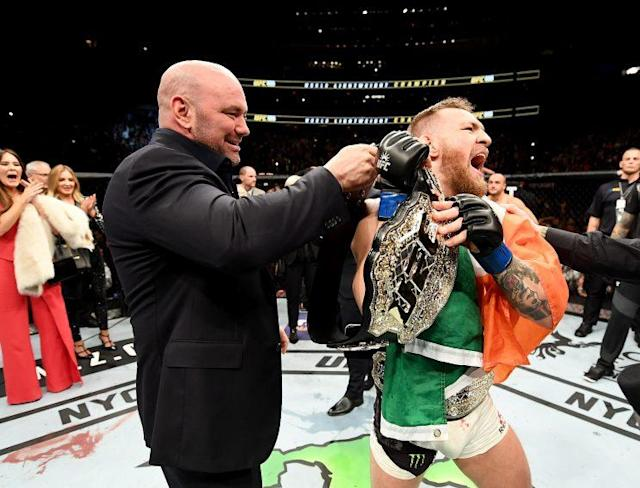
\includegraphics[trim={5cm 0 0 0.8cm} ,clip,width=.725995\textwidth]{templates/me.jpg}

\end{figure}

/joke
Lupe Fiasco, for inspiration, Nick Cambi for perspiration, and Inky Johnson for motivation.

joe jack Cathy Karen Dow (mit general services)
Ernie Kelsey
Tami
Messina
Rice
Miskimen
Joe (service guy from UMass)
All JLab hockey guys
Elton Smith JLab
the tech guy from JLab that was fat and crazy
Thesis Peter Charles axel Fabian jlab people
Fridericke Jentoft
Jan, ross, frank taylor for thesis

I'd like to take this chance to acknowledge


\graphicspath{ {./images/} }

The universe is immense and it seems to be homogeneous, 
in a large scale, everywhere we look at.



\begin{figure}[hbt]
	\centering
	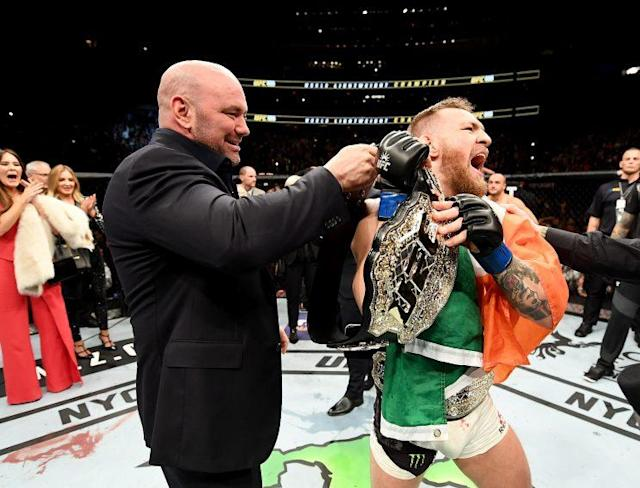
\includegraphics{templates/me.jpg}
\end{figure}


absolutely nobody


\fi



 
% Some departments (e.g. 5) require an additional signature page.  See
% signature.tex for more information and uncomment the following line if
% applicable.
% % -*- Mode:TeX -*-
%
% Some departments (e.g. Chemistry) require an additional cover page
% with signatures of the thesis committee.  Please check with your
% thesis advisor or other appropriate person to determine if such a 
% page is required for your thesis.  
%
% If you choose not to use the "titlepage" environment, a \newpage
% commands, and several \vspace{\fill} commands may be necessary to
% achieve the required spacing.  The \signature command is defined in
% the "mitthesis" class
%
% The following sample appears courtesy of Ben Kaduk <kaduk@mit.edu> and
% was used in his June 2012 doctoral thesis in Chemistry. 

\begin{titlepage}
\begin{large}
This doctoral thesis has been examined by a Committee of the Department
of Chemistry as follows:

\signature{Professor Jianshu Cao}{Chairman, Thesis Committee \\
   Professor of Chemistry}

\signature{Professor Troy Van Voorhis}{Thesis Supervisor \\
   Associate Professor of Chemistry}

\signature{Professor Robert W. Field}{Member, Thesis Committee \\
   Haslam and Dewey Professor of Chemistry}
\end{large}
\end{titlepage}


\pagestyle{plain}
\tableofcontents
%\addcontentsline{toc}{chapter}{\listfigurename}
\newpage
\listoffigures
\newpage
\listoftables
\newpage
\newlistof{myequations}{equ}{\listequationsname}
\listofmyequations
\addcontentsline{toc}{chapter}{\listequationsname}





%%%%%%%%%%%%%%%%%%%%%%%%%%%%%%%%%%%%%%%%%%%%%%%%%%%%%%% BODY %%%%%%%%%%%%%%%%%%%%%%%%%%%%%%%%%%%%%%%%%%%%%%%%%%%%%%%%%%%%
\chapter{Introduction} \label{Chapter:Intro}
\section{Exploring Structure through Scattering}\label{ch1:sec1:background}

Humanity interested in the structure of reality, atomic theory, subatomic, subnuclear, structure of this thesis.  The rest of this chapter discusses these advancments, and describes the theoretical background for this experiment. Chapter 2 descriptes the experiment, CHapter 5 the analysis, etc. Chapter 8 summarizes this work and discusses how this analysis will proceed in the near future and a path for future experiments. The appendix includes numerous technical details and upplemental plots.

As we increase the resolution (resolve features over smaller spatial distances), what we see is dependent on what resolution scale we are at. An exception to this case is if we are investigating point-like particles, which would have an identical response across all resolution scales

GPDs combine the kinematics of both elastic form factors and parton distributions. Andrey references 5, 6, and 7

\subsection{Discovery of the Proton}
Yimin has good references for this part
\subsection{Electron as a Nucleon Probe}

Include discussion of wavelength and momentum transfer (but in practice, limiting factor to resolution is lens system %https://advanced-microscopy.utah.edu/education/electron-micro/%

1961 hofstadter nobel prize (Andrey reference 1)
Andrey refrence 2 Friedman Kendall Tayleor scaling

Andrey thesis good write ups

Sangbaek:
proton has properties
Describe with QFT, words about QCD
role of experiment in studying proton structure
- proton discovery
- neutron discovery
- pointlike consitutents
- development of quark model
- scaling behavior and asymptotic freedom
- details about scattering experiments from first principles
- words about elastic scattering (mott scattering)
- Plot of elastic form factors, discussion of Ge and Gm, Rosenbluth formula
- Mention TPEX
- discussion of inelastic scattering
- Structure funcitons
- Discussion of spin and sum rules

Now discussion of DVEP:
GPDs, Wigner functions
relationships all the way around
some annoying math
Handbag diagram
Lepton hadron plane
Status of experiments and future (EIC mapping)




%Maybe someone will tell you to include something about the standard model



invariant mass is W 




Understanding the structure of matter has been a fundamental research pursuit for centuries. 


Proton not a point mass - it has structure



    \subsection{Structure of our World}
    - atomic theory
    - discovery of proton / nucleon
    - proton structure measurements
    - lepton scattering experiments, HERA, etc


\section{Theoretical Background}
    Discussion of Form Factors and genralized proton structure, Wigner Functions
    
    \subsection{GPDs and Deeply Virtual Scattering}

          The cross section for DV$\pi^0$P has been theoretically linked to GPDs, which describe the 3D structure of the nucleon.

    
     \begin{equation}\label{DVPiPXCrossSection}
           \frac{d^4\sigma_{\gamma^*p \rightarrow p'\pi^0}}{dQ^2dx_Bdtd\phi_{\pi}} =
         \Gamma (Q^2, x_B, E)
         \frac{1}{2\pi}
         \left\{ \left(  \textcolor{sigmaT}{\frac{d\sigma_T}{dt}}+\epsilon  \textcolor{sigmaL}{\frac{d\sigma_L}{dt}} \right)+
         \epsilon cos(2\phi)  \textcolor{sigmaTT}{\frac{d\sigma_{TT}}{dt}} + 
         \sqrt{2\epsilon(1+\epsilon)} cos(\phi)  \textcolor{sigmaLT}{\frac{d\sigma_{LT}}{dt}} \right\}
     \end{equation}
     
    There are 8 GPDs, 4 correspond to helicity conserving (chiral even) processes and 4 correspond to are helicity flipping (chiral odd) processes: \GPDH,  \GPDE,  \GPDHtilde,  and \GPDEtilde for chiral even, and \GPDHT,  \GPDET,  \GPDHTtilde, and \GPDETtilde \\
\GPDETbar = 2*\GPDHTtilde+\GPDET is commonly used

    
    \begin{table}[H]
        \centering
        \begin{tabular}{@{} *{4}{c} @{}}
                \headercell{Nucleon \\ Polarization} & \multicolumn{3}{c@{}}{Quark Polarization}\\
                \cmidrule(l){2-4}
                & U & \textcolor{white}{lllll}L & T    \\ 
                \midrule
                  U  & \GPDH &                                   &  \GPDETbar \\
                  L  &                    &  \textcolor{white}{llll}\GPDHtilde &                                   \\
                  T  & \GPDE &                                   &  \GPDHT,\GPDHTtilde \\
            \end{tabular}\\
            
    \end{table}
    


    
    Why do the scrtucture combine in the way they do with the coefficents of cos phi terms and epsilons?
    
    And the structure functions can be written as:

    \begin{equation}
         \textcolor{sigmaL}{\frac{d\sigma_{L}}{dt}} = 
        \frac{4\pi\alpha}{kQ^2}\left\{ \left( 1 - \xi^2 \right) 
        \lvert \langle \GPDHtildeEQ \rangle \rvert ^2 
        -2\xi^2 \Re \left[  \langle \GPDHtildeEQ \rangle ^* \langle \GPDEtildeEQ \rangle    \right] - \frac{t'}{4m^2}\xi^2
        \lvert \langle \GPDEtildeEQ \rangle \rvert ^2  \right\}
    \end{equation} 
  
    \begin{equation}
        \textcolor{sigmaT}{\frac{d\sigma_{T}}{dt}} = 
        \frac{2\pi\alpha \mu_{\pi}^2}{kQ^4}
        \left\{ \left( 1 - \xi^2 \right) 
        \lvert \langle \GPDHTEQ \rangle \rvert ^2
        - \frac{t'}{8m^2}
        \lvert \langle \GPDETbarEQ \rangle \rvert ^2  \right\}    
    \end{equation} 
    
    \begin{equation}
        \textcolor{sigmaLT}{\frac{d\sigma_{LT}}{dt}} = 
        \frac{4\pi\alpha \mu_{\pi}}{\sqrt{2}kQ^3}
        \xi\sqrt{1-\xi^2}
        \frac{\sqrt{-t'}}{2m}
        \Re \left\{ 
         \langle \GPDHTEQ \rangle ^*
        \langle \GPDEtildeEQ \rangle   
        \right\}
     \end{equation} 
    
    
    \begin{equation}
        \textcolor{sigmaTT}{\frac{d\sigma_{TT}}{dt}} = 
        \frac{4\pi\alpha \mu_{\pi}^2}{kQ^4}
        \frac{-t'}{16m^2}
        \langle \GPDETbarEQ \rangle^2   
    \end{equation} 
        
    

    and epsilon is... 
    
    and t' stands for.. t - $t_0$ where $t_0 = \frac{-4m^2\xi^2}{1-\xi^2}$
    
    
    Where the skewness parameter is $\xi = \frac{x_B}{2-x_B}$ or whatever
    

    The bracket $\langle \tilde{F} \rangle$ is the convolution of a GPD and an appropriate subprocess amplitude:
    $
    \langle \tilde{F} \rangle =  \Sigma_{\lambda} \int_{-1}^{1} d\bar{x}H_{0\lambda,0\lambda}\left( \bar{x}, \xi, Q^2, t=0  \right)\tilde{F}\left( \bar{x}, \xi, Q^2, t  \right)\   
    $ 


    Where $\lambda$ is the unobserved helicites of the partons participaing in the subprocess
    
    
    
    
    And k is the phase space factor given as 
     \scalebox{0.7}{%
     $           k = 16\pi \left( W^2 -m^2)\sqrt{\Lambda(W^2,-Q^2,m^2)} \right)$ 
    }
    
        Where $\Lambda(W^2,-Q^2,m^2)$ is the Källén function and $\mu_{pi}$ is the reduced pion mass given as 
       \scalebox{0.7}{%
      $         \mu_{\pi^0} = \frac{m^2_{\pi^0}}{m_u+m_d}$ 
    }
    $m_u$ and $m_d$ are respective masses of up and down quarks.


        Include proton pressure distribution plot

      

    \begin{equation}
                 \Gamma (Q^2, x_B, E) = \frac{\alpha}{8\pi} \frac{Q^2}{m^2_pE^2}\frac{1-x_B}{x_B^3}\frac{1}{1-\epsilon}
    \end{equation}
In addition to collinear momentum distribution of partons inside the
nucleon, GPDs also encode the distribution of partons in the plane transverse to
the nucleons momentum in the infinite momentum frame [58]. Moreover, their
relation to energy-momentum tensor (EMT) form factors allow us to access the
EMT densities, the distribution of energy, angular momentum, pressure, and shear
forces inside the nucleon [15].

Only valence quarks contribute electroproduction of uncharged pions.

    \subsection{The Handbag Approach}

    

 DVMP is sensitive to chiral odd GPDs, distinguishing it from DVCS as a GDP probe because why? Because something involving photon helicity and pion helicity, I forget exactly though
 
    \subsection{The Goloskokov-Kroll Model}
    
\section{Overview of Experimental Status}
    \subsection{Previous Experimental Results}


    \subsection{Overview of this Analysis}
    
Hi \cite{Bedlinskiy2014} see more in section ~\ref{ch1:sec1:background}
just a test



\iffalse
    \subsection{Unused}
        The following is from a paper on pi+ production. This formula is equvalent to the normal convetion (not using W as a variable)
        
         \begin{equation}\label{xsec}
             \frac{d^4\sigma_{\gamma^*p \rightarrow p'\pi^0}}{dQ^2W^2dtd\phi_{\pi}} =
             \frac{\alpha (W^2-m^2)}{16\pi^2 E^2_L m^2 Q^2 (1-\epsilon)}
             ((\frac{d\sigma_T}{dt}+\epsilon\frac{d\sigma_L}{dt})+
             \epsilon cos(2\phi) \frac{d\sigma_{TT}}{dt} + \sqrt{2\epsilon(1+\epsilon)}cos(\phi)\frac{d\sigma_{LT}}{dt})
        \end{equation}
        
        Comparing the two, we have a difference in the prefactor of:
        
        0.3894 * 1E6 * $\frac{1}{16\pi(W^2-m_p^2)\sqrt{W^4 + (Q^2)^2+m_p^4+2W^2Q^2-2W^2m_p^2+2Q^2m_p^2}}$
        
        This factor is accounted for by the Kallen function phase space term.
        
        
        
        
        t' stands for.. t - $t_0$ where $t_0 = \frac{-4m^2\xi^2}{1-\xi^2}$
        
           Where the skewness parameter is $\xi = \frac{x_B}{2-x_B}$ 
           
        
        
            Where $\lambda$ is the unobserved helicites of the partons participaing in the subprocess
            
         and epsilon is... 
            
            
            
            
         
               
            And k is the phase space factor given as 
             \scalebox{0.7}{%
             $           k = 16\pi \left( W^2 -m^2)\sqrt{\Lambda(W^2,-Q^2,m^2)} \right)$ 
            }
            
                Where $\Lambda(W^2,-Q^2,m^2)$ is the Källén function and $\mu_{pi}$ is the reduced pion mass given as 
               \scalebox{0.7}{%
              $         \mu_{\pi^0} = \frac{m^2_{\pi^0}}{m_u+m_d}$ 
            }
            $m_u$ and $m_d$ are respective masses of up and down quarks.
            
             Where $\Gamma (Q^2, x_B, E)$ is the virtual photon flux, is 
             \scalebox{0.7}{%
                $         \Gamma (Q^2, x_B, E) = \frac{\alpha}{8\pi} \frac{Q^2}{m^2_pE^2}\frac{1-x_B}{x_B^3}\frac{1}{1-\epsilon}$ 
            }

\fi



\iffalse

\chapter{Lepton (electron) Scattering}
    \section{Overview}
        We can probe the structure of sub-atomic particles by shooting high energy particles at them. The higher the energy, the shorter distances we resolve. This was done for example in the early 1900s with Rutherford scattering, leading to the discovery of the nucleus in the atom.\\
        \indent For probing the structure of the proton, ideal scattering particles are leptons, as they are point particles with (apparently) no sub-structure themselves. Electrons are the simplest to use as they are stable and easy to produce, but muons and neutrinos are also used.\\
        \indent A key concept is that increasing the energy of the incident particle allows you to resolve shorter distances, which corresponds to different scattering cross sections as you change energy. The following plot illustrates this and is essential:\\
    
        \begin{figure}[H]
            \centering
            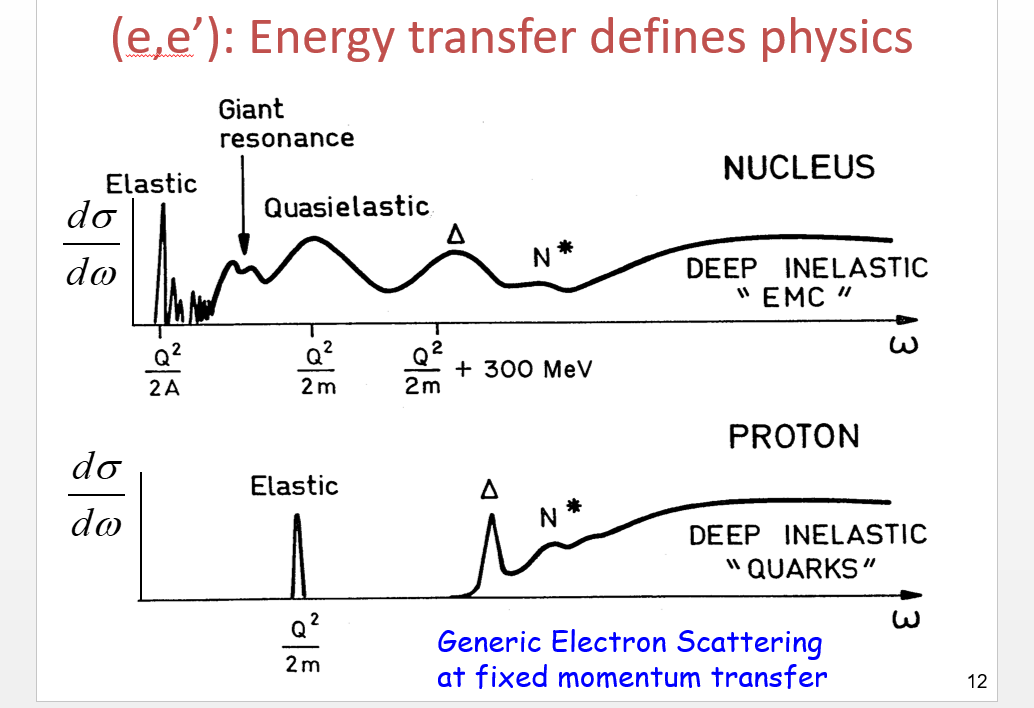
\includegraphics[width=10cm]{NuclearPhysics/modules/lepton-scattering/pics/e-p-scattering.png}
            \caption{Electron-proton scattering cross section vs. energy transfer $\omega$}
        \end{figure}
    \section{Quasi-Elastic}
        Quasielastic – is broadened due to fermi motion, also slightly shifted due to binding energy of nucleon in nucleus.
\chapter{Elastic Scattering}

    \section{Elastic Low Energy (Proton = Point) Limit: Rutherford and Mott Scattering}
        \indent Both Rutherford and Mott scattering neglect the proton recoil and treat the proton as a point source. \\
        \indent The Feynman calculations for this process are straightforward and carried through exactly in Thomson 7.2. \\
        
        \begin{figure}[H]
            \centering
            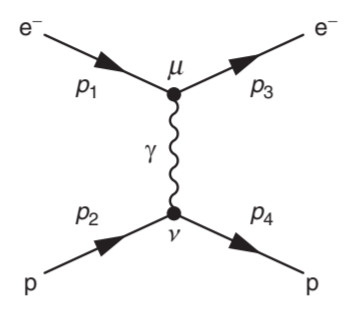
\includegraphics[width=10cm]{NuclearPhysics/modules/lepton-scattering/pics/elastic-ep/rut-1.PNG}
            \caption{Diagram for basic ep scattering}
        \end{figure}
        
        \begin{figure}[H]
            \centering
            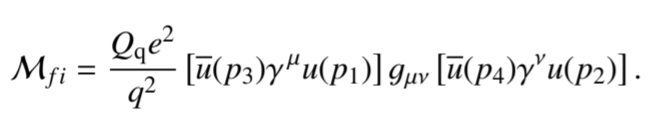
\includegraphics[width=8cm]{NuclearPhysics/modules/lepton-scattering/pics/elastic-ep/rut-matrix.PNG}
            \caption{Matrix element for ep scattering}
        \end{figure}
        
        \begin{figure}[H]
            \centering
            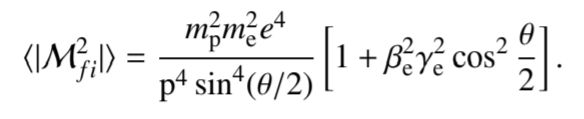
\includegraphics[width=6cm]{NuclearPhysics/modules/lepton-scattering/pics/elastic-ep/full-matrix.PNG}
            \caption{Result of matrix element calculation}
        \end{figure}
        
        \subsection{Rutherford scattering}
            \indent Rutherford scattering assumes the electron is non-relativistic, yielding a cross section of:

                \begin{equation}
                    \frac{d\sigma}{d\Omega} = \frac{\alpha^2}{16E^2_K\sin^4{(\theta/2)}}
                \end{equation}
                %\myequations{Rutherford Scattering}
            
            In this non-relativistic limit, only the interaction between the electric charges of the electron and proton contribute; there is no magnetic (spin-spin) interaction. The angular dependence originates only from the 1/$q^2$ propagator term.
            
        \subsection{Mott Scattering}
            \indent Mott scattering has a relativistic electron but still fixed point proton. Now since electron momentum is about equal to its energy, reductions lead to the Mott cross section:
            
                \begin{equation}
                    \frac{d\sigma}{d\Omega} = \frac{\alpha^2}{4E^2\sin^4{(\theta/2)}}\cos^2{\frac{\theta}{2}} = \left( \frac{\alpha}{2E\sin^2{(\theta/2)}}\cos{\frac{\theta}{2}} \right)^2
                \end{equation}
                %\myequations{Mott Scattering}
            
            Again, purely magnetic spin-spin interactions are negligible here. 
            
        \subsection{Summary}
            Rutherford - elastic scattering, proton = fixed, point, electron $\neq$ relativistic\\
            Mott - elastic scattering, proton = fixed, point, electron = relativistic
        
            \begin{equation}
                (\frac{d\sigma}{d\Omega})_{Mott} = 4\cos^2{\frac{\theta}{2}}(\frac{d\sigma}{d\Omega})_{Ruth}
            \end{equation}
    \section{Form Factors: Accounting for Proton Structure}
        \indent If the proton were a point, then the Mott Scattering cross section would agree with experiment for all electron scattering energies. Instead, deviations from Mott are observed as we increase the beam energy. To account for this structure, we need to define form factors, which describe the structure of the proton:
        
        \begin{equation}
            \frac{d\sigma}{d\Omega} = \frac{\alpha^2}{4E^2\sin^4{(\theta/2)}}\cos^2{\frac{\theta}{2}}(F(\textbf{q}^2))^2
        \end{equation}
        
        
        $F(\textbf{q}^2)$ is the 3D Fourier transform of the charge distribution: 
        
        \begin{figure}[H]
            \centering
            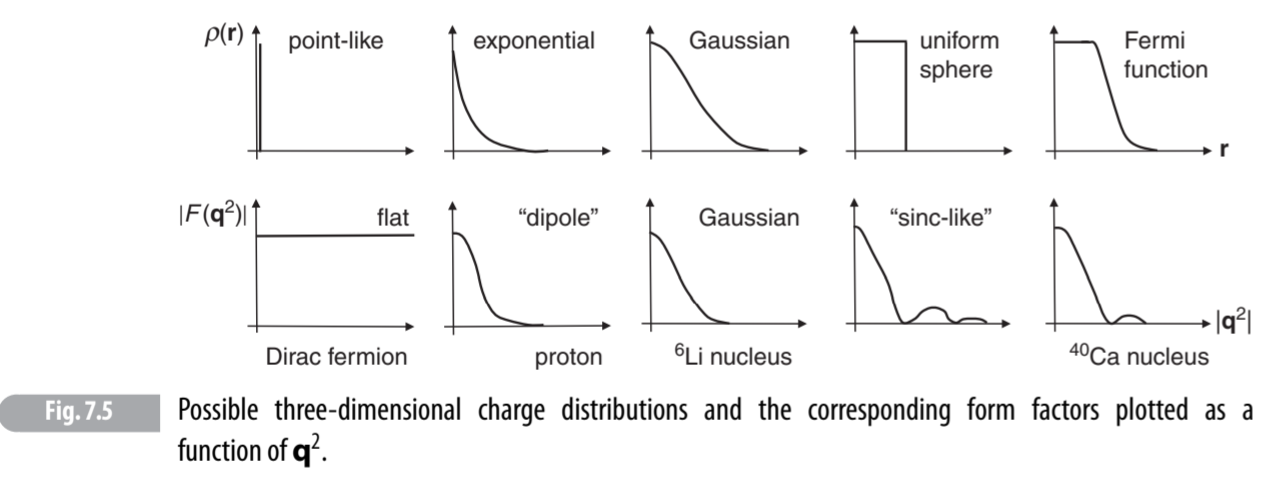
\includegraphics[width=14cm]{NuclearPhysics/modules/lepton-scattering/pics/elastic-ep/charge-dist.PNG}
            \caption{Charge Distribution Fourier Transforms}
        \end{figure}
        
        In general, a spin S particle will have 2S + 1 form factors. For example, a proton is spin 1/2, and has 2 form factors. A spin 3/2 particle will have 4 form factor (e.g. Li7) 
        
    \section{Relativistic Electron Proton Elastic Scattering}
        \indent Explicit math is worked out in Thomson 7.4 and is straightforward, but important relations are:
        
        \begin{figure}[H]
            \centering
            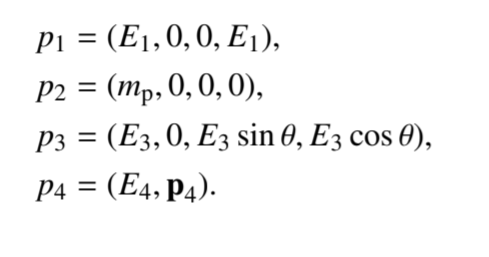
\includegraphics[width=6cm]{NuclearPhysics/modules/lepton-scattering/pics/elastic-ep/kine-e-1.PNG}
            \caption{Kinematic 4-vectors of particle momentum}
        \end{figure}
        
        \begin{figure}[H]
            \centering
            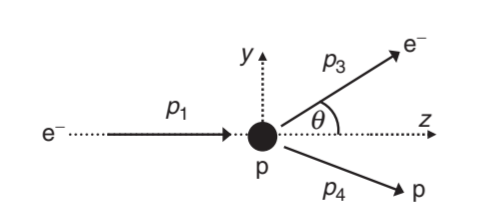
\includegraphics[width=10cm]{NuclearPhysics/modules/lepton-scattering/pics/elastic-ep/kine-e-2.PNG}
            \caption{Elastic scattering diagram}
        \end{figure}
        
        From the electron - photon - electron vertex, we get the four-momentum squared of the virtual photon (neglect the mass of the electron) $q^2$:
        
        \begin{equation}
            Q^2 = -q^2 = 4E_1E_3\sin^2(\frac{\theta}{2})
        \end{equation}
        
         We can $E_3$ expressed in terms of the scattering angle of the electron:
         
        \begin{equation}
            E_3 = \frac{E_1m_p}{m_p+E_1(1-\cos\theta)}
        \end{equation}
        
        This lets us rewrite $Q^2$ as:
        
        \begin{equation}
            Q^2 = \frac{2m_pE_1^2(1-\cos\theta}{m_p+E_1(1-\cos\theta)}\label{eq:2}
        \end{equation}
        %\myequations{$Q^2$ - Incident Electron Energy Relation, Elastic Scattering}
        
        Which gives us the differential cross section for the scattering of relativistic electrons from a pointlike proton as: 
        
        \begin{equation}
            \frac{d\sigma}{d\Omega} = \frac{\alpha^2}{4E_1^2\sin^4{(\theta/2)}}\frac{E_3}{E_1}(\cos^2{\frac{\theta}{2}}+\frac{Q^2}{2m_p^2}\sin^2(\frac{\theta}{2}))
        \end{equation}
       % \myequations{Elastic Scattering Cross Section - pointlike proton}
        
        \subsection{Important Notes}
            \indent Elastic ep scattering has only 1 independent variable, so measuring the scattering angle determines all of the kinematics. In practice, by measuring the energy and angle of scattered electrons, the system can be over constrained to ensure that the scattering was in fact elastic. \\

            \indent Compared to Mott Scattering, there are two differences in the elastic scattering formula. The $E_3/E_1$ term in the scattering cross section comes from the electron losing energy to the proton's final state kinetic energy (no longer a fixed source). The new term proportional to $\sin^2(\theta/2)$ is due to a purely magnetic spin-spin interaction. 
    \section{Rosenbluth}
        \indent The derived cross-section for elastic scattering still lacks any proton structure. To incorporate structure, we need to include two form factors, $G_E(Q^2)$ - related to the distribution of charge, and $G_M(Q^2)$, related to the distribution of the magnetic moment inside the proton. In the low-$Q^2$ limit, these form factors are the Fourier transforms of the charge an magnetic moment distributions, but the carryover is not exact in general due to being functions of the 4-momenta, instead of 3 momenta. E.g.:
        
        \begin{figure}[H]
            \centering
            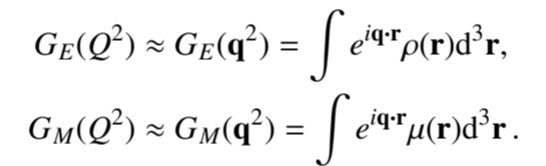
\includegraphics[width=6cm]{NuclearPhysics/modules/lepton-scattering/pics/elastic-ep/fourier-gegm.PNG}
            \caption{Interpretations of $G_E$ and $G_M$}
        \end{figure}
        
        Including these form factors in our cross section gives us the full elastic scattering cross section:
                
        \begin{equation}
            \frac{d\sigma}{d\Omega} = \frac{\alpha^2}{4E_1^2\sin^4{(\theta/2)}}\frac{E_3}{E_1}\left( \frac{G_E^2+\tau G_M^2}{1+\tau} \cos^2{\frac{\theta}{2}}+2\tau G_M^2\frac{Q^2}{2m_p^2}\sin^2(\frac{\theta}{2})\right)
        \end{equation}
       % \myequations{Full Elastic Scattering Cross Section}
        
        Here $\tau$ is:
                
        \begin{equation}
            \tau = \frac{Q^2}{4m_p^2}
        \end{equation}
        
        
        \subsection{Rosenbluth Separation - Measuring Ge and Gm}
            \indent By increasing our beam energy, we will see deviations away from Mott scattering behaviour. We see this explicitly by rewriting the scattering formula as:
            
            \begin{equation}
                \frac{d\sigma}{d\Omega} = \left( \frac{G_E^2+\tau G_M^2}{1+\tau} +2\tau G_M^2\tan^2(\frac{\theta}{2})\right) \left( \frac{d\sigma}{d\Omega}_0\right)
            \end{equation}
      %  \myequations{Full Elastic Scattering Cross Section}
        
        
        Where $\frac{d\sigma}{d\Omega}_0$ is the Mott Scattering cross section, with the factor of $\frac{E_3}{E_1}$ included to account for proton recoil. We can then extract $G_E$ and $G_M$ in the following way (\textbf{"Rosenbluth Separation"}):\\
        \subsection{Rosenbluth Method Walk through}
            \subsubsection{Take Data}
                1.) Experimental set up - electron beam scattering off of proton target. Could use something like GaAs source, Linac up to 0.1 - 1 GeV, incident on proton target, liquid hydrogen should be fine. For a detector, use a dipole spectrometer with scintillating tile focal plane, or something else to measure position well (MWPC, (cheap) silicon strips (expensive, good resolution)). You want to measure the electrons energy so you know $E_3$, e.g. you want to be able to over constrain the event so you know it was in fact elastic. Other than that you are just counting events.\\
                
                2.) Put spectrometer at 135 degrees in theta from the beam axis. Take data at 10 different beam energies. You know know the cross section at that angle at that energy. Now move the spectrometer to 120 degrees. Repeat energy scan. Repeat this process for several other beam angles. You are done taking data.
            \subsubsection{Analyze data}
                1.) Go into your data. Using the relation between $Q^2$, $\theta$, and $E_1$, pick a value of $Q^2$ (e.g. 0.292 GeV$^2$, invert to find the beam energy at the appropriate $\theta$, and note the cross section at that point. What you just did is find the cross-section value at that angle, corresponding to a specific $Q^2$ value. Repeat for all the angles you had your spectrometer at. You now have a plot of cross section vs. angle ($\tan(\theta^2)$ so that it is a line), at a specific $Q^2$ value. \\
                2.) Now fit a line to the data. The slope gives you $G_M$ at that $Q^2$, and the y-intercept gives you $G_E$ at that $Q^2$ (see \label{eq:1})\\
                3.) Repeat steps 1 and 2 for as big of a $Q^2$ range that you can. \\
                \newline
                Side notes from Axel - the Rosenbluth method has awful systematics - need to measure absolute cross sections, radiative corrections become large, uncertainties for $G_E$ and $G_M$ are correlated, etc.
            \subsubsection{Results}
                Carrying out this procedure gives you plots of $G_E$ and $G_M$ vs. $Q^2$. 
                
                We see as $Q^2$ goes to zero, we recover $G_E$ = 1 and $G_M$ = 2.79, as it should. The data fits well to the so called "dipole function" i.e.:
                \begin{figure}[H]
                    \centering
                    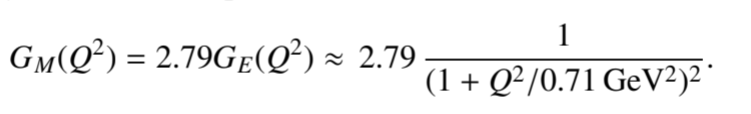
\includegraphics[width=8cm]{NuclearPhysics/modules/lepton-scattering/pics/elastic-ep/dipole.PNG}
                    \caption{Rosenbluth Results}
                \end{figure}
                This relates to a proton charge distribution as exponentially falling off, i.e.\\
                $\rho(r) \sim \rho_0 e^{-r/a}$\\
                Here a = 0.24 fm, which corresponds to a proton RMS charge radius of 0.8 fm. \\
                Finally, at high $Q^2$, $G_M \propto Q^{-4}$, which means that the elastic scattering cross section falls as $1/Q^6$
                Also, we can calculate the RMS charge radius of the proton as:
                
             
                \begin{figure}[H]
                    \centering
                    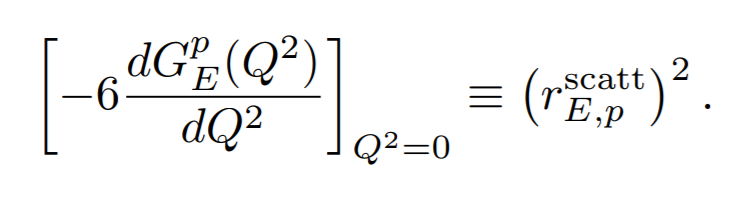
\includegraphics[width=6cm]{NuclearPhysics/modules/emc-src-scaling/pics/prad-GE.PNG}
                \caption{Taylor expansion of $G_E$ to yield proton charge radius}
                \end{figure}
    \section{Olympus and TPEX}
        The Rosenbluth method of measuring the ratio of $G_E$ and $G_M$ has awful systematics, based mainly in the facts that you need to measure an absolute cross section, worry about radiative corrections, and measure at low $Q^2$. A better way to measure the proton form factor ratio is by a \textbf{polarization transfer} measurement. This uses a \textbf{Focal Plane Polarimeter} to converst transverse polarization into an azimuthal distribution:
        
              
        \begin{figure}[H]
            \centering
            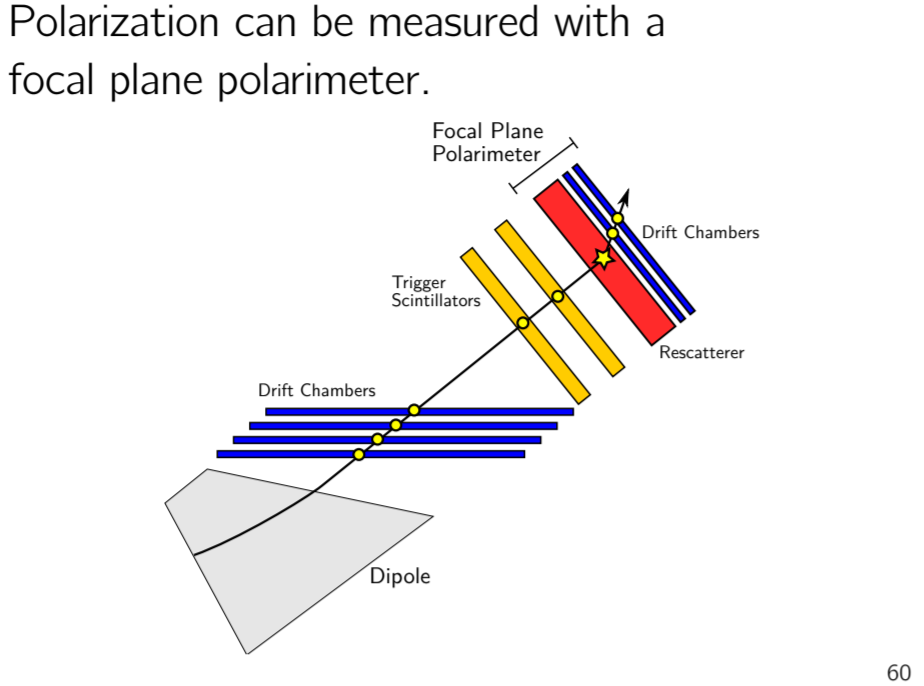
\includegraphics[width=10cm]{NuclearPhysics/modules/lepton-scattering/pics/elastic-ep/olympus-fpp.PNG}
            \caption{Olympus experimental setup}
        \end{figure}
        
        This method has the advantages that we are measuring a ratio, not an absolute cross section, so many uncertainties cancel, such as the FPP analyzing power. Olympus produced the following:
        
              
        \begin{figure}[H]
            \centering
            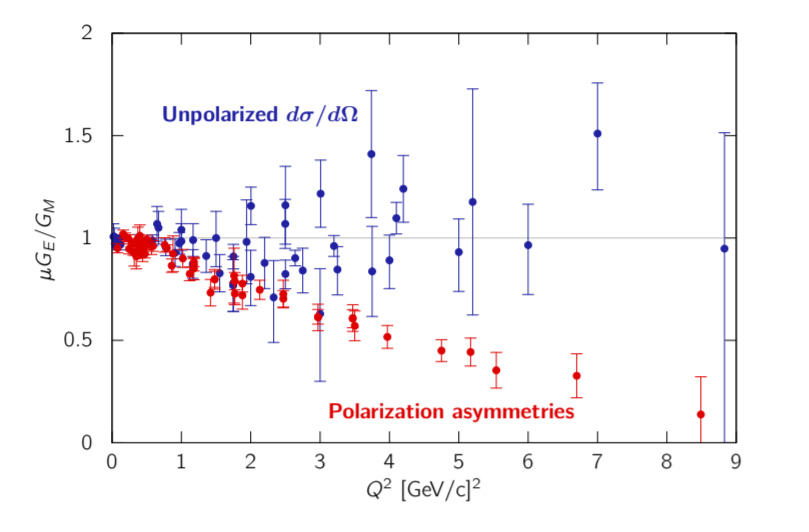
\includegraphics[width=10cm]{NuclearPhysics/modules/lepton-scattering/pics/elastic-ep/olympus-form-factors.PNG}
            \caption{$G_E$ and $G_M$ ratio measurements}
        \end{figure}
        
        This discrepancy may be due to two photon exchange, which we can measure by comparing electron to positron scattering:
        
              
        \begin{figure}[H]
            \centering
            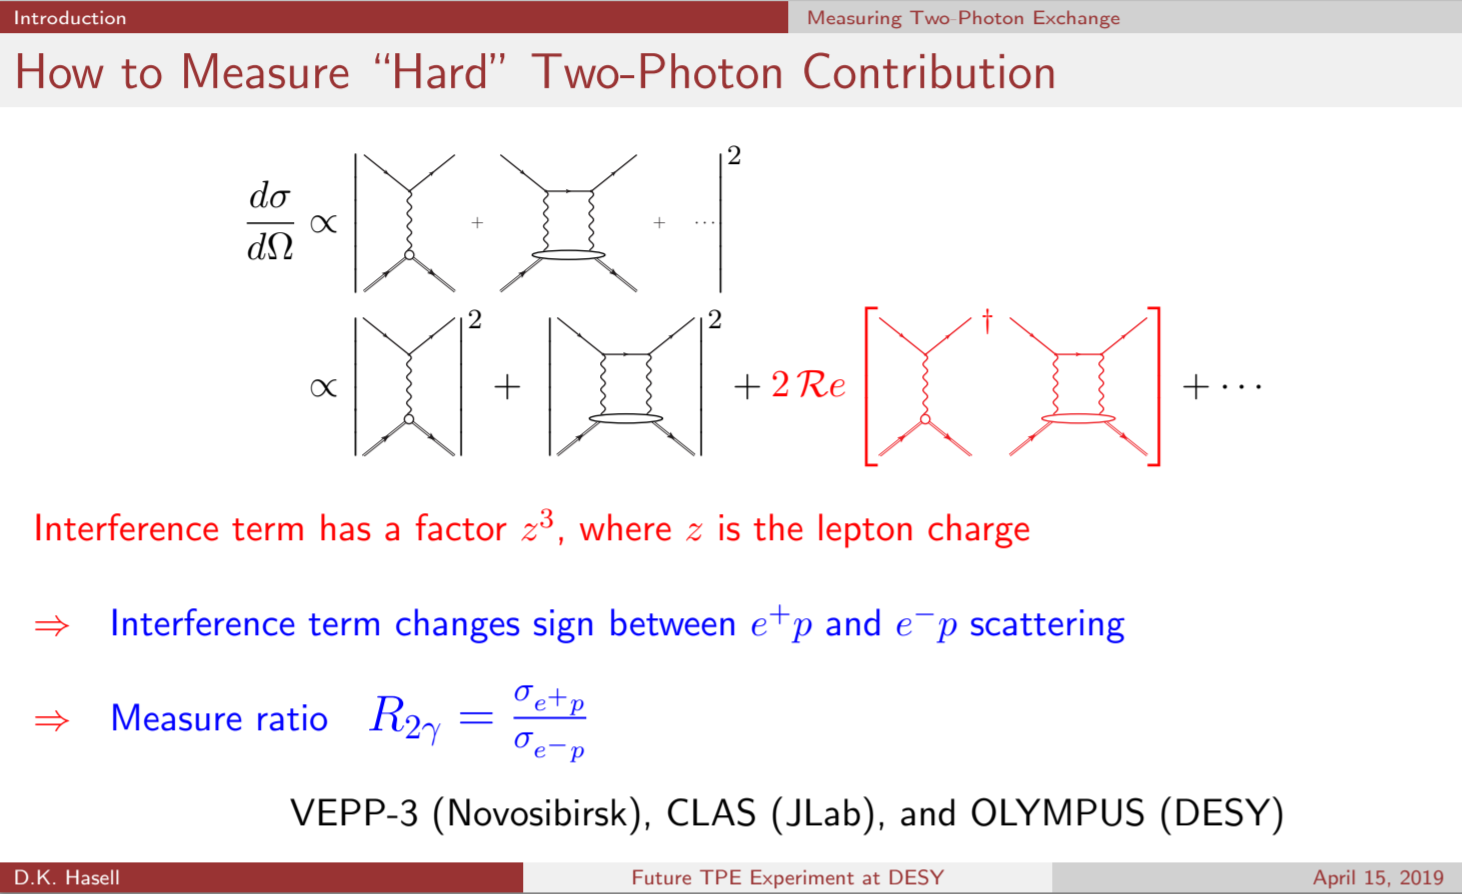
\includegraphics[width=10cm]{NuclearPhysics/modules/lepton-scattering/pics/elastic-ep/tpex.PNG}
            \caption{Electron Positron charge interference}
        \end{figure}
    
    
        TPEX is a currently proposed experiment to extend this out to farther $Q^2$, which is challenging due to its lower luminosity of elastic scattering as $Q^2$ increases.     
       
\chapter{Inelastic Scattering}
    \section{Overview}
        In inelastic scattering, we now no longer require that the proton remains intact, and we can create resonances, or as we increase the energy, can create a slew of hadronic final states. Since we remove the constraint that the mass of the final state is the proton mass, we now have one extra degree of freedom, i.e., we need 2 variables to describe inelastic scattering. These are usually Bjorken X $x_B$ and the 4-momentum transfer of the virtual photon $Q^2$.\\
        N.B. - 1990 Nobel Prize awarded to Friedman, Kendall, and Taylor "for their pioneering investigations concerning deep inelastic scattering of electrons on protons and bound neutrons, which have been of essential importance for the development of the quark model in particle physics"
    \section{Variables}
                
        \subsection{Bjorken X}
        Think of Xb as the ratio of momentum transfer to energy transfer. 
        
        $x_B$ is a measure of elasticity - 1 for elastic scattering. Also, is the fraction of proton momentum carried by the struck quark in the infinite momentum frame.
        \begin{equation}
            x = \frac{Q^2}{2p_2\cdot q} = \frac{Q^2}{Q^2+W^2-m_p^2}
        \end{equation}
        %\myequations{Bjorken X}
    
            Derivation of infinite momentum frame Bjorken x. Take quark to have momentum fraction $\xi$ of proton's total momentum,i.e. $p_q = \xi p_2$:\\
            \indent Inf. Mom. frame - neglect proton mass so $p_2$ = $E_2$, neglect all transverse momenta:\\
            \indent Struck quark 4-momenta: $p_q = \xi p_2 = (\xi E_2, \xi E_2, 0, 0)$\\
            \indent 4-momenta of quark after interaction: $(p_q + q) = (\xi p_2 +q)$\\
            \indent Square the 4-momenta $(\xi p_2 +q)^2 = \xi^2 p_2^2 +q^2 + 2\xi p_2 \cdot q  = m_q^2$\\
            \indent Continue, noting $p_q = \xi p_2$ : $m_q^2 = p_q^2 - Q^2 + 2 \xi p_2 \cdot q$\\
            \indent Since $p_q^2$ = $m_q^2$, we have: $m_q^2 = m_q^2 -Q^2 + 2 \xi p_2 \cdot q$\\
            \indent So $0 = -Q^2 + 2\xi p_2 \cdot q \longrightarrow \xi = \frac{Q^2}{2 p_2 \cdot q} = x_B$\\
        
        
        \subsection{Y}
        y is a measure of the inelasticity of the scattering, it is the fractional energy lost by the electron in the scattering process (second equality is true where proton is at rest). 0 is for perfectly elastic, 1 is for entirely inelastic. 
        
        \begin{equation}
            y = \frac{p_2 \cdot q}{p_2 \cdot p_1} = 1 - \frac{E_3}{E_1}
        \end{equation}
        
        \subsection{Q2}
        With these variables, we can make the equality for $Q^2$:
        
          \begin{equation}
            Q^2 = (s-m_p^2)xy \sim sxy
        \end{equation}
        
        Since you are now breaking up the proton, you have an additional degree of freedom, so you need two observables to describe inelastic scattering. 
        

        \subsection{W}
            W is the four momenta of the final state system that started with the proton, W = q + $p_2$. It is useful as $W^2 = m_p^2 -Q^2 + 2 p_2 \cdot q$
        
    \section{Deep Inelastic Scattering}
        \indent To describe further proton sub-structure, we need to introduce structure functions, $F_1(x,Q^2)$ - purely magnetic, and $F_2(x,Q^2)$. For DIS where $Q^2 >> m_p^2y^2$, we have the following cross section formula:
        
        \begin{figure}[H]
            \centering
            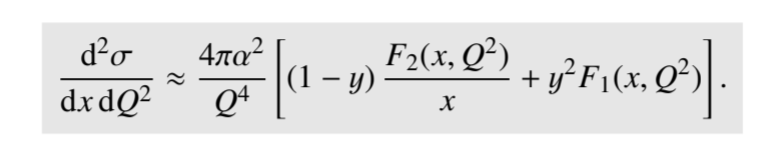
\includegraphics[width=10cm]{NuclearPhysics/modules/lepton-scattering/pics/inelastic-ep/dis-xsection.PNG}
            \caption{General DIS cross section}
        \end{figure}
    \section{Bjorken Scaling and Callan Gross}
        \indent In DIS, we observe Bjorken scaling and Callan-Gross
        
        \begin{figure}[H]
            \centering
            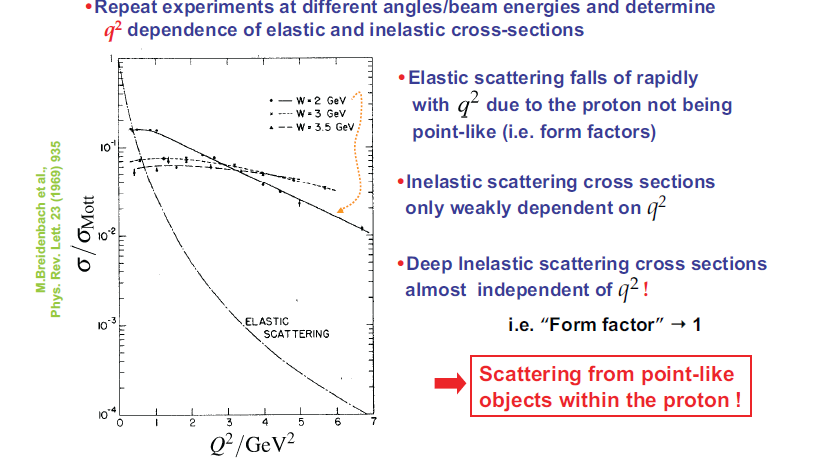
\includegraphics[width=10cm]{NuclearPhysics/modules/lepton-scattering/pics/inelastic-ep/DIS.png}
            \caption{Early Bjorken Scaling Example}
        \end{figure}
        
        After performing DIS measurements at SLAC with electron energies between 5 and 20 GeV on liquid hydrogen, using a movable spectrometer over various angles, showed two important results:\\
        \newline
        \textbf{Bjorken Scaling} where $F_1$ and $F_2$ are basically flat with respect to $Q^2$, and thus are independent of $Q^2$, indicating that we are scattering off point-like constituents inside the proton.\\
        \newline
        \textbf{Callan Gross Relation} where $F_2 = 2x F_1$, a relation which can be explained by assuming the underlying process is actually elastic scattering off of point-like spin-half constituents inside the prton (quarks). 
    \section{Structure Functions and Parton Distribution Functions}
        \indent These describe the distribution of quarks within the nucleon. Describes the momentum fraction distribution of quarks. For example:\\
        \newline
        $u^p(x)dx$\\
        \newline
        Represents the number of up-quarks within the proton with momentum fraction between x and dx. The functional forms of the PDFs are not a-priori known. Some potential PDFs could be as shown below:\\
        
        \begin{figure}[H]
            \centering
            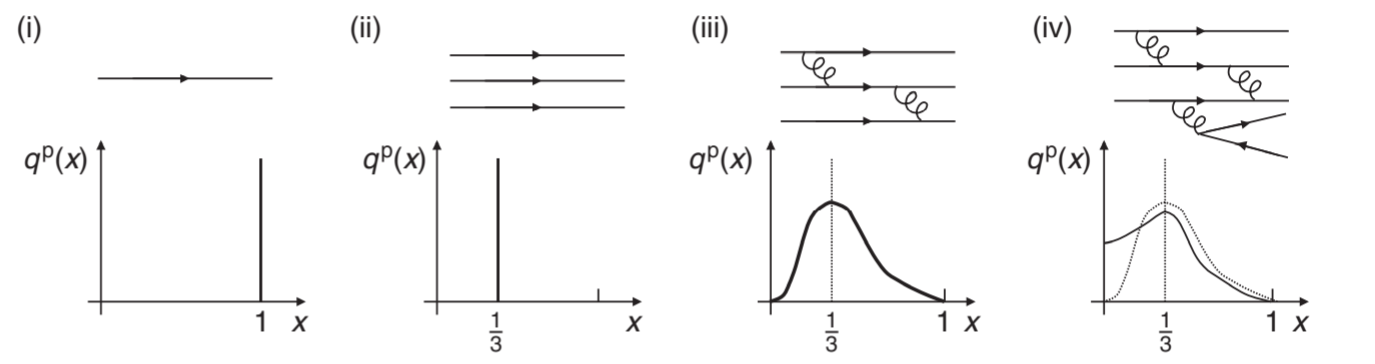
\includegraphics[width=12cm]{NuclearPhysics/modules/lepton-scattering/pics/inelastic-ep/pdf-possibilities.PNG}
            \caption{Potentail PDFs}
        \end{figure}
        
        (i) - if the proton consisted of a single quark\\
        (ii) - if the proton had 3 static quarks\\
        (iii) - quarks interacting and Heisenberg uncertainty (momentum smearing)\\
        (iv) - interacting quarks with higher order diagrams - gluons produced, so enhances low x part of PDF\\
        \newline
        We can access these distributions experimentally as the parton model predicts the the cross section for elastic scattering off of quarks with charge $Q_i$ and momentum fraction in the range of x to x + dx as:
        
               
        \begin{figure}[H]
            \centering
            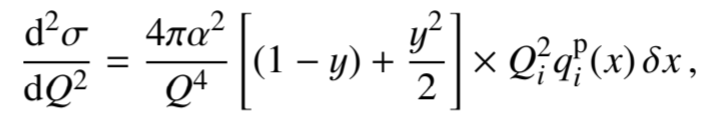
\includegraphics[width=8cm]{NuclearPhysics/modules/lepton-scattering/pics/inelastic-ep/quark-x.PNG}
            \caption{Quark scattering cross section}
        \end{figure}
        
        So then the cross section summing over all quark flavours is:
        
               
        \begin{figure}[H]
            \centering
            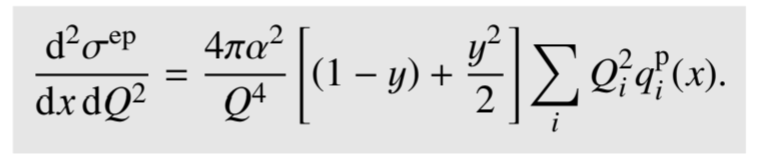
\includegraphics[width=8cm]{NuclearPhysics/modules/lepton-scattering/pics/inelastic-ep/quark-x-sum.PNG}
            \caption{Quark PDF - cross section relation}
        \end{figure}
        
        and comparing it with the general expression for DIS cross section:
        
                
        \begin{figure}[H]
            \centering
            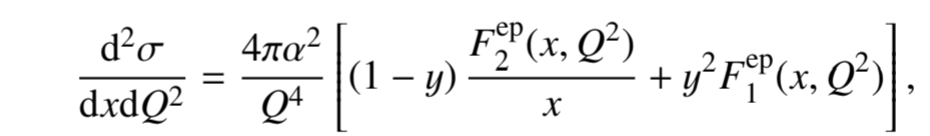
\includegraphics[width=8cm]{NuclearPhysics/modules/lepton-scattering/pics/inelastic-ep/inel-general.PNG}
            \caption{General DIS cross section}
        \end{figure}
        We see we can get the relation:
        
                
        \begin{figure}[H]
            \centering
            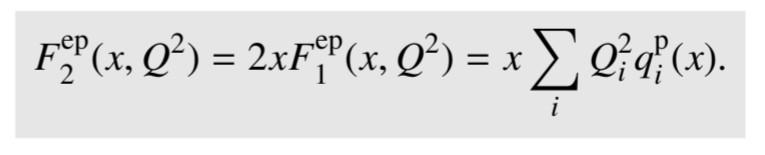
\includegraphics[width=8cm]{NuclearPhysics/modules/lepton-scattering/pics/inelastic-ep/f2-sum-q.PNG}
            \caption{Structure function - quark PDF relatio}
        \end{figure}
        
        For an explicit example, we have (neglecting heavier quarks, which have smaller contributions):
        
                
        \begin{figure}[H]
            \centering
            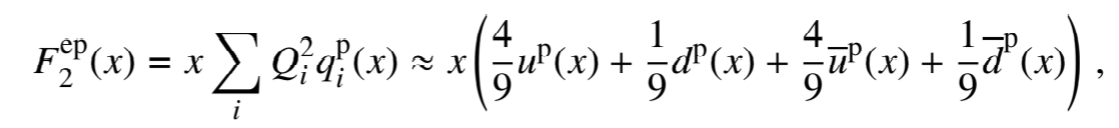
\includegraphics[width=12cm]{NuclearPhysics/modules/lepton-scattering/pics/inelastic-ep/example-f2.PNG}
            \caption{Up and Down quark contributions to structure functions}
        \end{figure}
        
        Note that the parton model predicts both Bjorken scaling and the Callan Gross relation. Importantly, because QCD is hard, the PDFs cannot be calculated from perterbation theroy, and must be measured in DIS. We can integrate the PDFs to determine the total momentum fraction of the proton carried by each flavour of quark, as:
        
                
        \begin{figure}[H]
            \centering
            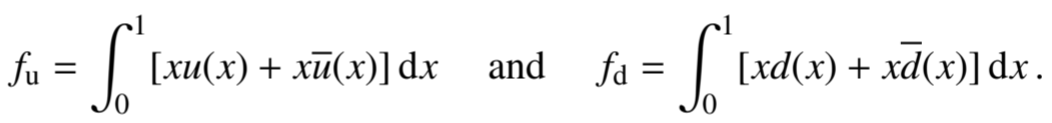
\includegraphics[width=12cm]{NuclearPhysics/modules/lepton-scattering/pics/inelastic-ep/integrated-ud.PNG}
            \caption{Total quark momentum fractions}
        \end{figure}
        
        Doing this after DIS measurements yields $f_u = 0.36$ and $f_d = 0.18$, so the u and d quarks only carry about half of the total momentum of the proton. The rest is carried by gluons, which do not interact in QED ep scattering. \\
        
        There are other predictions to be made here, such as the ratio of $F_2$ in neutrons vs. in protons. It would be expected that the ratio would go to 1 as $x_B$ goes to 0, as at low x the PDF is dominated by sea quarks and gluons, which are independent of nucleon type. At high $Q^2$ we would expect some ratio as basically the number f up quarks to down quarks, but this is not what is seen; instead we observe a modification which might be explained by the fact that it is more likely to have one up quark at high momentum, as if the one down quark were at high momentum, the two up quarks would be closer in phase space, which is disfavoured by the Pauli Exclusion principle. 
    \section{Scaling and Violations}
        Structure functions were studied in great detail (one million DIS events at $Q^2$ greater than 200 GeV$^2$ - kinematic range was up to $Q^2 = 20,000 GeV^2$ and $x < 0.0001$. $Q^2$ and $x$ were determined solely by precisely measuring the scattering angle and energy of the electron. 
        
        \begin{figure}[H]
            \centering
            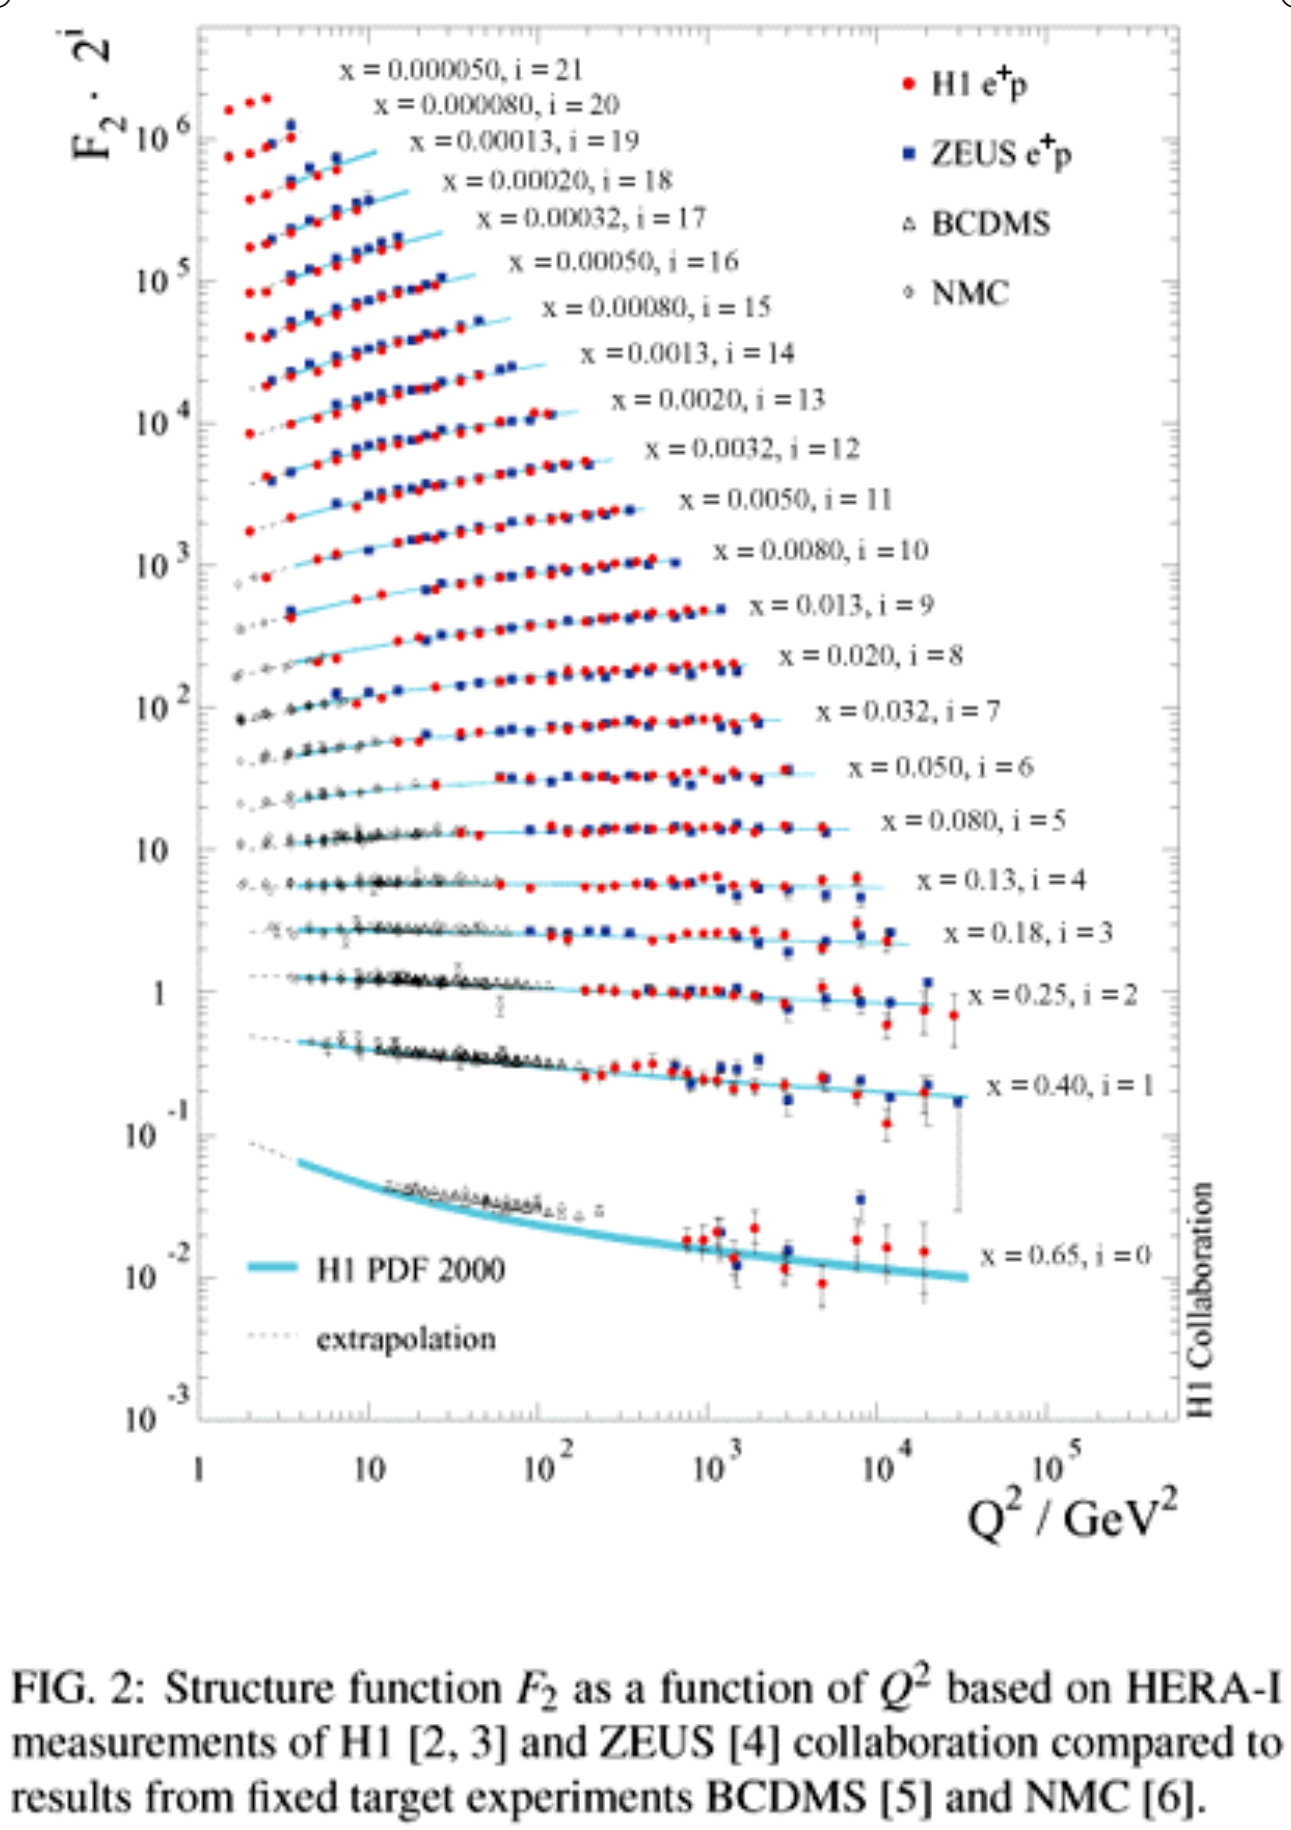
\includegraphics[width=10cm]{NuclearPhysics/modules/lepton-scattering/pics/inelastic-ep/Hera-dis.PNG}
            \caption{HERA structure functions}
        \end{figure}
        
        2 important takeaways:\\
        \newline
        1- Bjorken scaling holds up to $Q^2 = 20,000$ GeV$^2$, implying that quarks are point like up to scales of at least $10^{-18}$m. \\
        \newline
        2- \textbf{Scaling violations: }\\
        \newline
        \indent At medium X, we are independent of Q2, indicating we have quarks. At high x, the $F_2$ structure function decreases at high x, and increases at low x, with increasing $Q^2$. More specifically, imagine measuring the $F_2$ structure function across x at a certain $Q^2$. Now measure again at a higher $Q^2$. You will see the curve is shifted higher at low x, and lower at high x:
        
                
        \begin{figure}[H]
            \centering
            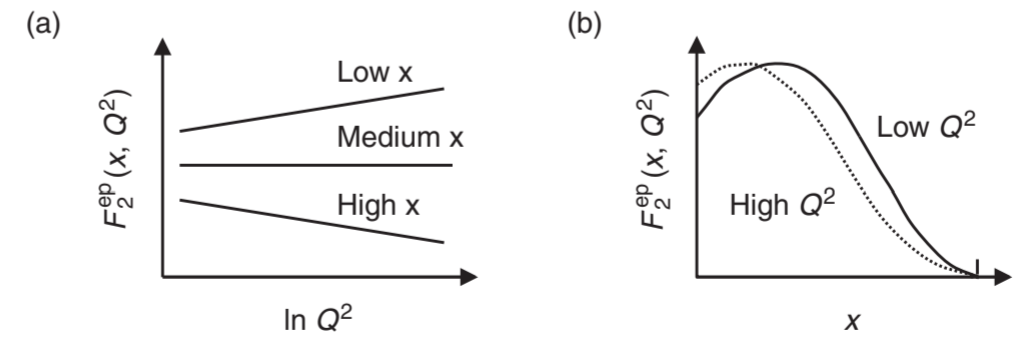
\includegraphics[width=12cm]{NuclearPhysics/modules/lepton-scattering/pics/inelastic-ep/scaling-violations.PNG}
            \caption{Explaination of Scaling Violations}
        \end{figure}
        
        This is indicative of the fact that at higher $Q^2$, the proton has a greater fraction of low x quarks. I.e., at low $Q^2$ we do not "see" the low-x quarks, but as we increase our resolving power, we do.\\
        \newline
        N.b. - we cannot measure the gluon PDFs, but can model them with QCD parton evolution equations such as DGLAP or BFKL.\\
        \newline
        Finally, we include a proton PDF at $Q^2$ = 10 GeV$^2$ and at $10^4$ GeV$^2$. (note - on a semilog plot!)
        
               
        \begin{figure}[H]
            \centering
            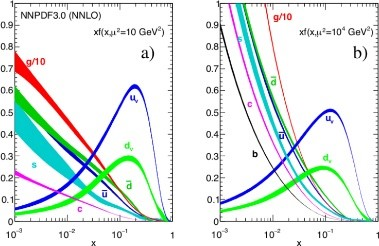
\includegraphics[width=14cm]{NuclearPhysics/modules/lepton-scattering/pics/inelastic-ep/PDFs.jpg}
            \caption{PDFs at two different $Q^2$ values}
        \end{figure}
     
 

\chapter{Jefferson Lab and CLAS12 Experimental Setup}
    \section{JLab 12 GeV CEBAF Machine}
        \subsection{Injector}
        \subsection{Accelerator and Beam Structure}
            What was the deal with looking into the time structure of the beam at JLab? Jan 2020
            Is beam polarized?
        \subsection{Other notes and comparison to CERN}
\chapter{Other Halls}
    \section{Hall A}
        \subsection{General Layout}
        \subsection{Tritium Experiment Notes}
        \subsection{BDX}
        \subsection{DVCS and DVMP Notes}
    \section{Hall C}
        \subsection{Who Cares}
    \section{Hall D}
        \subsection{Overview}
            \begin{figure}[H]
                \centering
                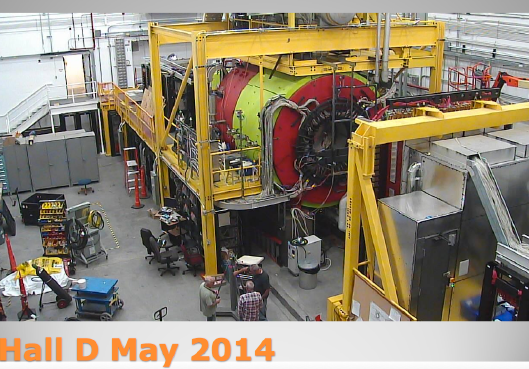
\includegraphics[width=8cm]{CLAS-12/modules/jlab/Other_Halls/HallD/Hall_Design/Hall_D.PNG}
                \caption{Hall D Overview with Solenoid}
            \end{figure}
            
            Hall D is located on the other side of the other 3 Halls at JLab and gets one extra Linac run, so is the only one able to receive the full 12 GeV beam. This hall actually uses a photon beam instead of an electron beam, as described below. The main experiments here are GlueX, PrimeX, Charged Pion Polarizability Experiment, etc.
            
        \subsection{Photon Beam Production and Structure}
            \begin{figure}[H]
                \centering
                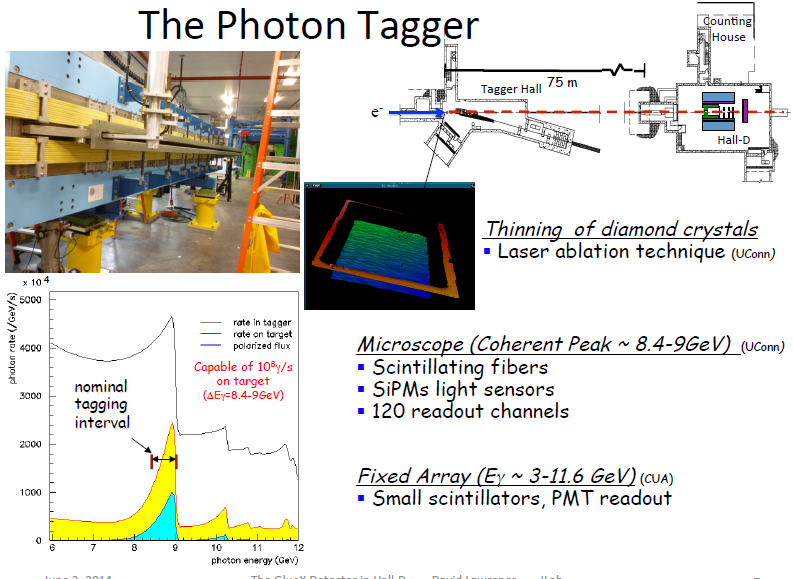
\includegraphics[width=14cm]{CLAS-12/modules/jlab/Other_Halls/HallD/Hall_Design/hall_D_Photon_tagger.PNG}
                \caption{Hall D Coherent Bremm. Photon Beam}
            \end{figure}
            
            \subsubsection{glue x pair spectrometers}
            \subsection{polarization measurement - triplet spectrometers?}
            
        \subsection{GlueX Detector Specifications}
            \begin{figure}[H]
                \centering
                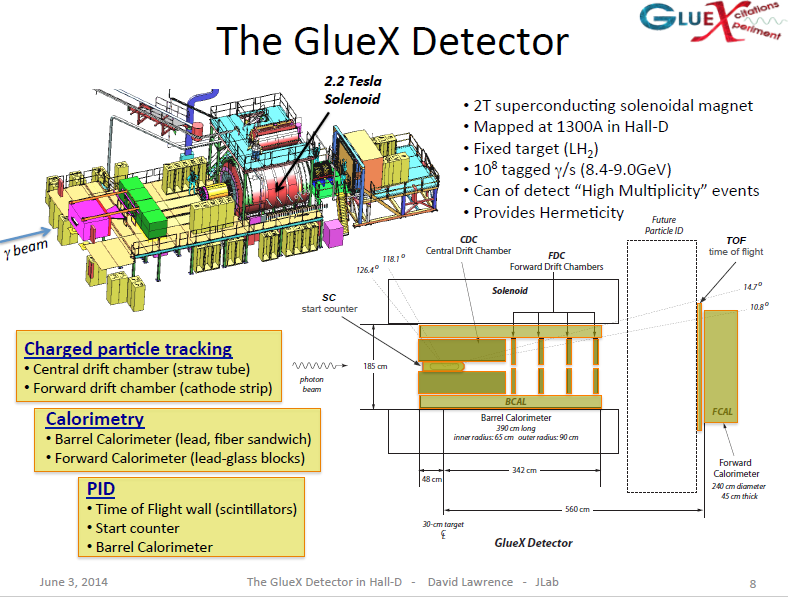
\includegraphics[width=12cm]{CLAS-12/modules/jlab/Other_Halls/HallD/Hall_Design/GlueX_Detector.PNG}
                \caption{Hall D GlueX Detector}
            \end{figure}
            
            
            CDC -  60/40 Ar/CO2 - 28 layers total - FADC 125 MHz -  resolution - $\sigma_{r\phi}$ = 150 $\mu m$
            $\sigma_{z}$ = 1.5 mm\\
            FDC - resolution 200 $\mu m$\\
            FCAL - 2800 lead glass blocks 4 x 4 x 45 $cm^3$ - PMT readout - resolution - $\frac{\sigma_E}{E} = \frac{5.7}{\sqrt{E}} + 2\%$ 
            
            \begin{figure}[H]
                \centering
                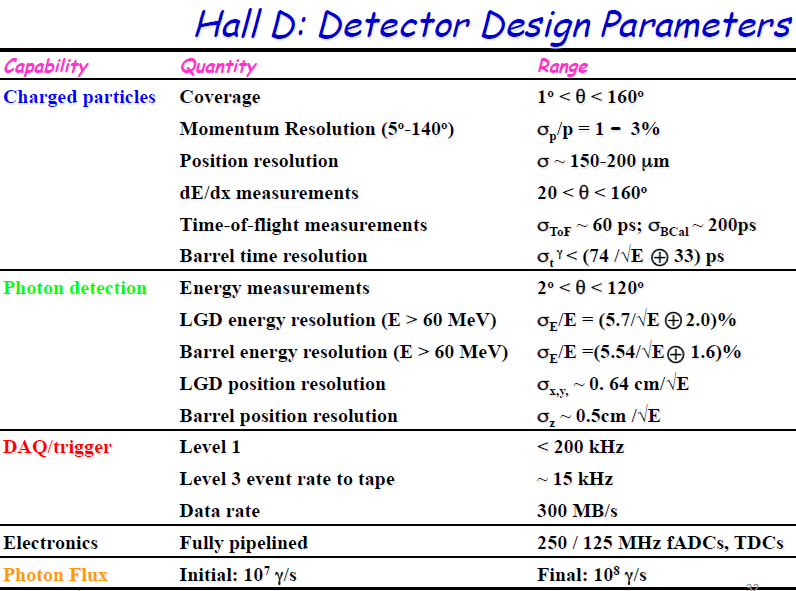
\includegraphics[width=8cm]{CLAS-12/modules/jlab/Other_Halls/HallD/Hall_Design/hall_d_design_params.PNG}
                \caption{Hall D GlueX Detector Design Specifications}
            \end{figure}
            
        \subsection{Example Experiment: Charge Pion Polarizability}
        Electric and Magnetic polarizabilities ($\alpha_{\pi}$ and $\beta_{\pi}$) are fundamental properties of particles with structure, such as the pion. In the low energy sector of QCD they can be related to the pion form factors $F_A$ and $F_V$. Leading order calculations from ChPT calculate $\alpha_{\pi}$ and $\beta_{\pi}$ to be equal in magnitude. 
        
        \begin{figure}[H]
            \centering
            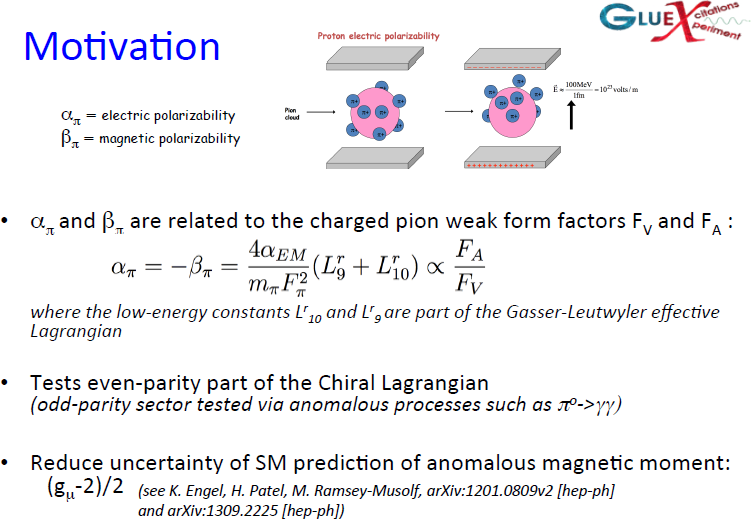
\includegraphics[width=12cm]{CLAS-12/modules/jlab/Other_Halls/HallD/cpp/cpp_motivation.PNG}
            \caption{Explanation for CPP Experiment}
        \end{figure}
            
        Experiments have been done to measure these quantities, but they do not agree with each other or ChPT:
            
        \begin{figure}[H]
            \centering
            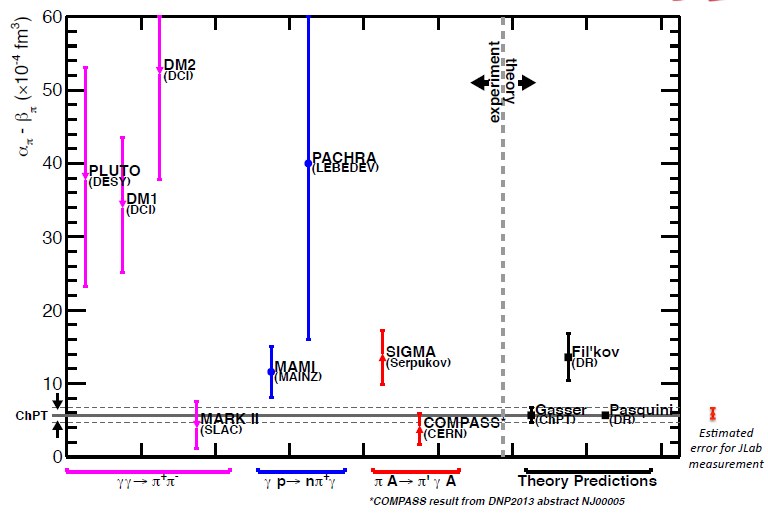
\includegraphics[width=12cm]{CLAS-12/modules/jlab/Other_Halls/HallD/cpp/cpp_motivation_plot.PNG}
            \caption{Phase Space Plot of CPP Experiments}
        \end{figure}
        
        Thus, the CPP experiment is proposed to run at glueX via the Primakoff effect ($\gamma \gamma \longrightarrow \pi \pi$. The polarizabilites will be measured as the cross section depends on these values, a factor of two difference results in a $\sim$ 10\$ diffference in cross section.
            
            \begin{figure}[H]
                \centering
                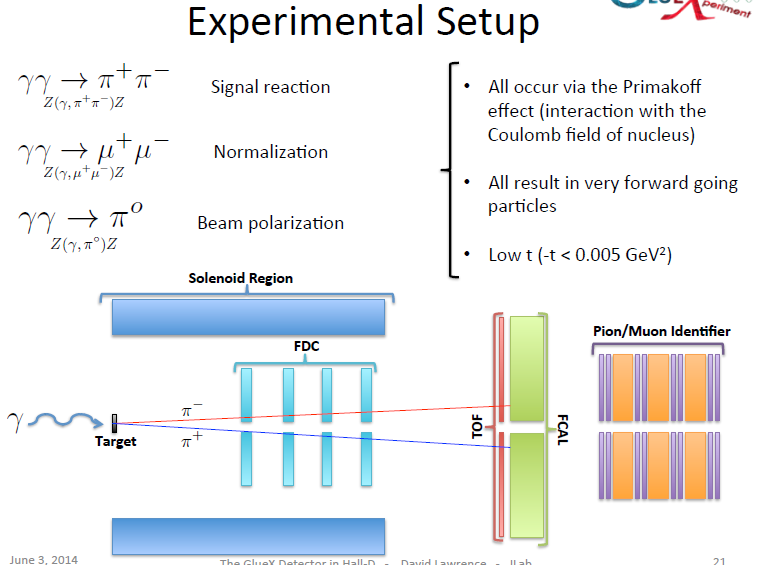
\includegraphics[width=12cm]{CLAS-12/modules/jlab/Other_Halls/HallD/cpp/cpp_experiment_setup.PNG}
                \caption{Experimental Setup for CPP Measurement}
            \end{figure}
            
            
            
            
            
            
            
\href{https://www.jlab.org/Hall-B/clas12-web/}{Detector specs here}     


            
          
          
\iffalse          
\subsection{GLUEX From Yunjie}
    I’ve heard that the oral exams this semester are all over Zoom, and pass/no record, which is nice, so you might as well just give it a shot and be done with it. I completely see what you are saying — it gets boring after a while studying it every single day! I assume you plan to do a practice sometime after you get your topic and do some reading on it? I’ll certainly tune in and provide feedback.
    
    For GlueX and/or DIRC, I agree that I don’t think they are going to be harsh about it, if they are going to ask anything at all. Nonetheless, it doesn’t hurt to know some basics. I happened to have given a student seminar talk about a year ago on GlueX+DIRC basics. I just uploaded it to the LNS students’ Oral Exam Google Drive under my personal folder, which may or may not be helpful but you can take a look.
    
    DIRC
    why it is useful to have a DIRC detector at all? I.e., why not just use a TOF or a normal cherenkov detector? 
    
    The short answer/bottom line is: GlueX physics program needs PID capabilities for K/pi separation up to 4 GeV. Our current TOF only goes up to ~ 2 GeV. We could have built a normal Cherenkov detector (i.e. it would meet our goal), but getting the BaBar DIRC is cheaper/easier(?) and does the job.
    
    Let me expand a little bit. 
    
     - Why PID? or K/pi separation for GlueX?
    The goal of the main GlueX physics program is to search for and eventually map out the hybrid meson spectrum. To do that, you need to produce and map out strange-quark-containing hybrid mesons as well. Those strange-quark-containing hybrid mesons presumably like to decay into a bunch of kaons (K+/-, K_long, K_short). People did the study and found that we need sufficient K/pi separation power (i.e. differentiating K+ from pi+, K- from pi-) up to 4 GeV.
    
    - Why not TOF?
    It cannot do the job. Our TOF timing resolution is about ~100 ps, and ~5 meters downstream of target. Actually, it’s a good exercise that they could’ve asked you during an exam to calculate the K/pi separation capability based on the timing resolution and distance. Give it a try and convince your self.
    
    - Why not a normal Cherenkov detector?
    I think we could’ve done that, but since DoE already has the DIRC bars sitting there from the decommissioned BaBar, and they studied it, and found that the DIRC can do the job and is cheaper.
    
    I assume there is some kind of advantage which makes it particulalry useful for BaBar and GlueX
    This was never formally explained to me by anyone, but I think I know the answer. For BaBar, yes, there’s a good reason: it’s very difficult to put a normal RICH type detector in the barrel region for good reasons. BaBar was a collider experiment with solenoid field design. To put RICH in the barrel region, you would need to put the whole RICH system inside, which increases the material budget and degrades the energy resolution, which is downstream. Also, PMTs don’t like magnetic fields (although you could try SiPM, but I wasn’t sure if it was available).
    
    Photon beam
    Short answer: yes, it’s probably easier to produce them in a real photon beam and also it’s easier to control the polarization of a real photon beam than that of the virtual photons in electron scattering.
    
    I think you are right that the cross section in a real photon beam is much higher. One of the most-targeted-for exotic mesons is the 1-+ state, e.g. page 9 of the slides. And photons have quantum numbers 1- -, which is a good start in that you only need to flip one quantum number, so the production cross section is likely high.
    
    Another important reason is polarization. In an electron beam, I actually don’t know how well you can control the polarization of the exchanged virtual photon, but for a real photon beam, it’s an experimental observable. Polarization is important because the silver bullet to identify those exotic mesons is their quantum numbers. To measure quantum numbers, if you can control the incoming photon beam in a polarized state, then you can basically play games like analyzing your data with different photon polarization states and show the properties of the presumably produced exotic meson follow exactly what you expect. Since I mentioned it here, I will just add something that you probably know already. If you are ever asked about things along the lines of determining quantum numbers (especially spin), it’s always good to say something along the lines of measuring the spatial/angular distributions of the decay products.
    
    I think this is likely more than enough for you to know about DIRC and GlueX. But let me know if you want to know more/anything is not clear!
    
\fi

\chapter{CLAS12 System}
    \section{Overview}
        \subsection{Introduction}
            The CLAS12 detector is a large angle spectrometer that generally covers angles from 5 to 130 degrees, spanned by two main detector subsystems - the Forward Detector and the Central Detector.
            
                
    		\begin{figure}[H]
    			\centering
    			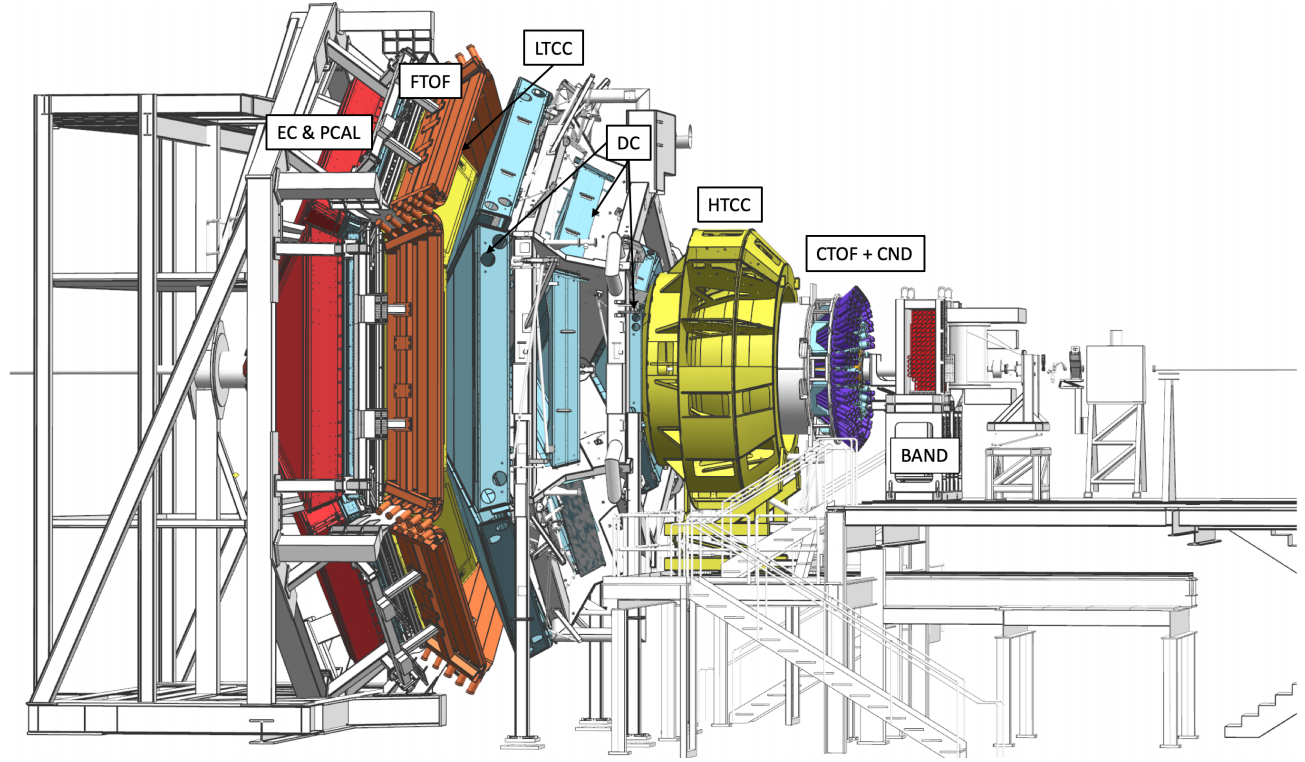
\includegraphics[width=12cm]{CLAS-12/modules/clas-12-system/pics/other/CLA12.PNG}
    			\caption{ CLAS12 Detector System }
			\end{figure}
			
        	\begin{figure}[H]
    			\centering
    			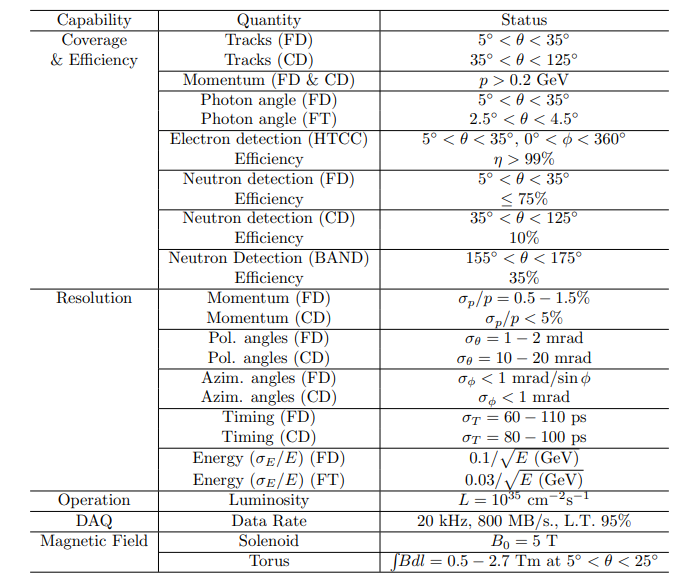
\includegraphics[width=10cm]{CLAS-12/modules/clas-12-system/pics/other/clas12-params.PNG}
    			\caption{CLAS12 Specification}
			\end{figure}
		
			\begin{figure}[H]
    			\centering
    			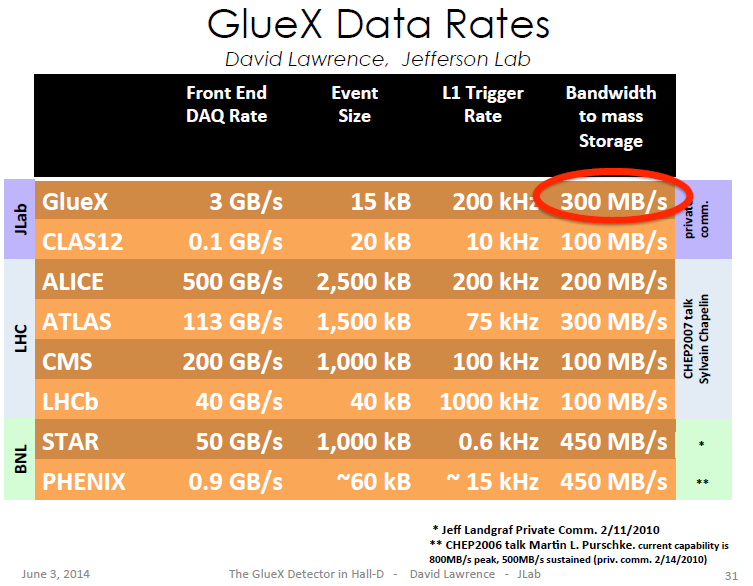
\includegraphics[width=10cm]{CLAS-12/modules/clas-12-system/pics/other/good_data_rates_slide.PNG}
    			\caption{CLAS12 Data Rates, Compared to Other Experiments }
			\end{figure}
    
    \section{Target and Other}
        \subsection{Beam from JLab}
                For entry into CLAS12, the beamline specs are as follows:\\
                Beam current: up to 50 nA\\
                Beam energy spread: $10^-4$\\
                Beam size: Less than 0.4 mm\\
                Beam stability: Less than 0.1 mm\\
                Beam halo: $10^-4$\\
                Beam polarization: up to 80\%\\
        \subsection{Liquid Hydrogen Target}
            \indent The hydrogen target in RGA is cooled to 20 K using a He4 evaporation fridge. Can by polarized by dynamic nuclear polarization, driven by a 140 GHz microwave source, can reach 90\% polarization for protons, 40\% for deuterons (both longitudinally polarized). The polarization can be measured by a Q-meter based NMR. 2.5 cm diameter target, extended 5 cm long. \\
            \indent RGA does not use a polarized target. The beam is polarized, but the target is not, so polarization is not helpful for extracting the 5-fold differential cross section (but it would be if the target was also polarized, and is useful for BSA measurements).
        \subsection{Luminosity Measurement}
            Luminosity in CLAS12 is measured from the Faraday Cup and using reference reactions such as elastic scattering. We don't use the Faraday Cup event by event, but we do use it run by run. For beam current measurements, beam position monitors upstream are used - but this is for monitoring on-line, not for analysis.
        \subsection{Moller Polarimeters}
            As stated, for RGA, the fact that the beam is polarized is not useful, but it is true and is measured by Moller Polarimeters. 
        
            \begin{figure}[H]
    			\centering
    			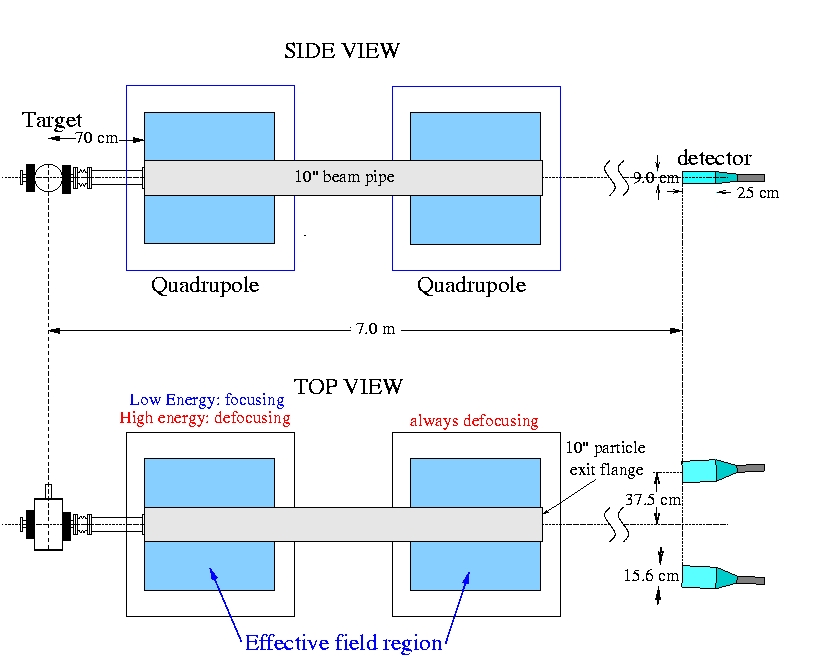
\includegraphics[width=12cm]{CLAS-12/modules/clas-12-system/pics/other/hall-b-poll-1.jpg}
    			\caption{ }
			\end{figure}
			
												
			 \begin{figure}[H]
    			\centering
    			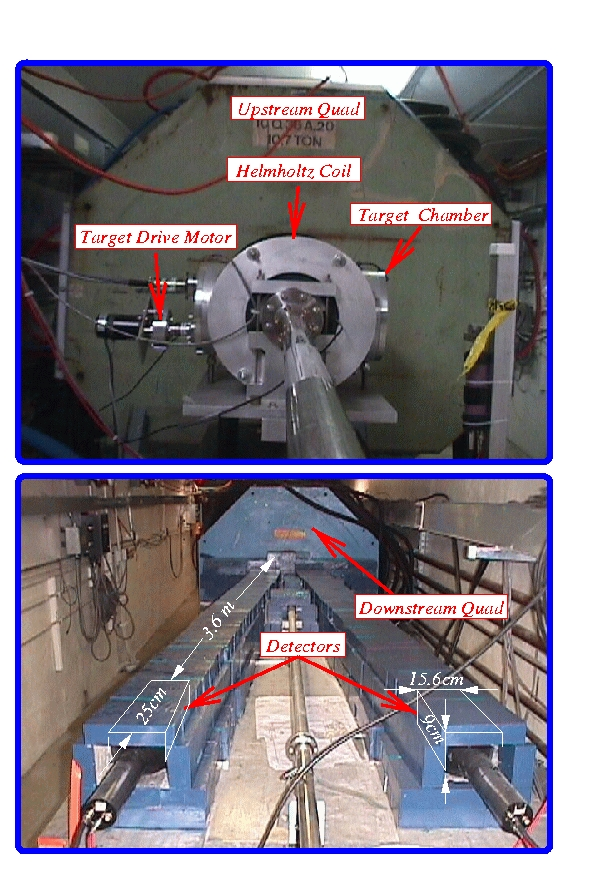
\includegraphics[width=12cm]{CLAS-12/modules/clas-12-system/pics/other/hall-b-poll-2.jpg}
    			\caption{ }
			\end{figure}
			
			 \begin{figure}[H]
    			\centering
    			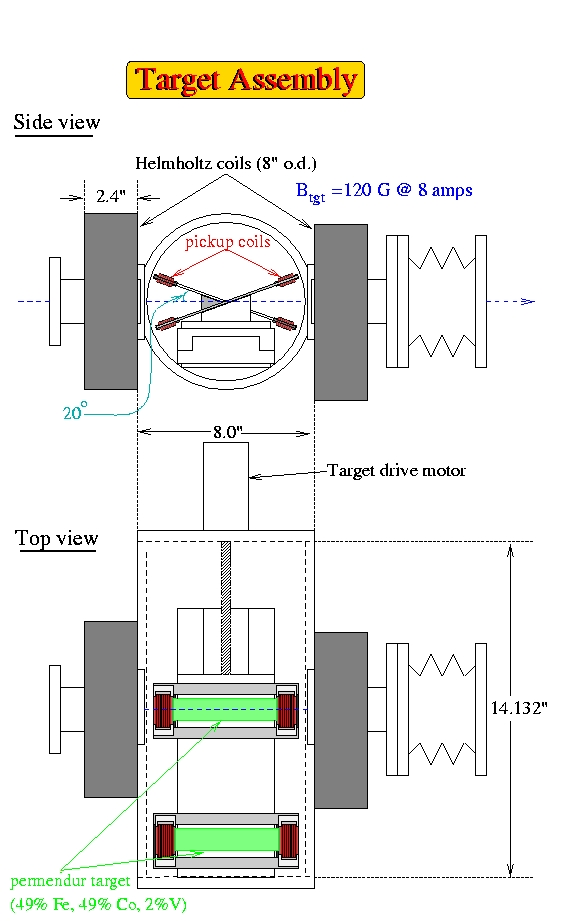
\includegraphics[width=12cm]{CLAS-12/modules/clas-12-system/pics/other/hall-b-poll-target.jpg}
    			\caption{ }
			\end{figure}
        \subsection{Trigger}
            CLAS12 runs with "open trigger", which means different sub-experiments can define their own triggering logic. There is a standard electron trigger, based off of hits in HTCC, ECal, and FTOF. 
  

        
        \subsection{Faraday Cup}
            Can manage 175 Watts - 17 nA at 10 GeV. Is used to calibrate beam current, needs a blocker in at higher currents.
            
    \section{Central Detector}
        Overview: The Central Detector spans roughly 35 to 125 degrees, and contains 4 sub-detectors, all in a 5 Tesla solenoidal field. The 5 detectors are: SVT, MMVT, CTOF, and CND. 
        \subsection{SVT}
            The Silicon Vertex Tracker (SVT) covers from 35 to 125 degrees in $\theta$. Has 8 layers (4 concentric rings) with 10, 14, 18, and 24 sectors respectively, double sided. 2$\pi$ angular coverage. Read out with ASICs- FSSR2s. Designed to operate at $10^{35}$ luminosity, momentum resolution of $\sim$ 5\% for 1 GeV particles with $\theta$ = 90 degrees. 42 cm long, 4 cm wide, 0.4 cm thick. Spatial resolution of 50 $\mu$m, momentum resolution $\sim$ 5\%, theta resolution 10 mrad, phi resolution 5 mrad.  33,792 total readout channels. Sensor thickness is 320 $\mu$m, readout pitch 156 $\mu$ m.Supported by rohacell and carbon fiber backing to reduce material budget, at $\sim 1\%$ of a radiation length.
            
            \begin{figure}[H]
    			\centering
    			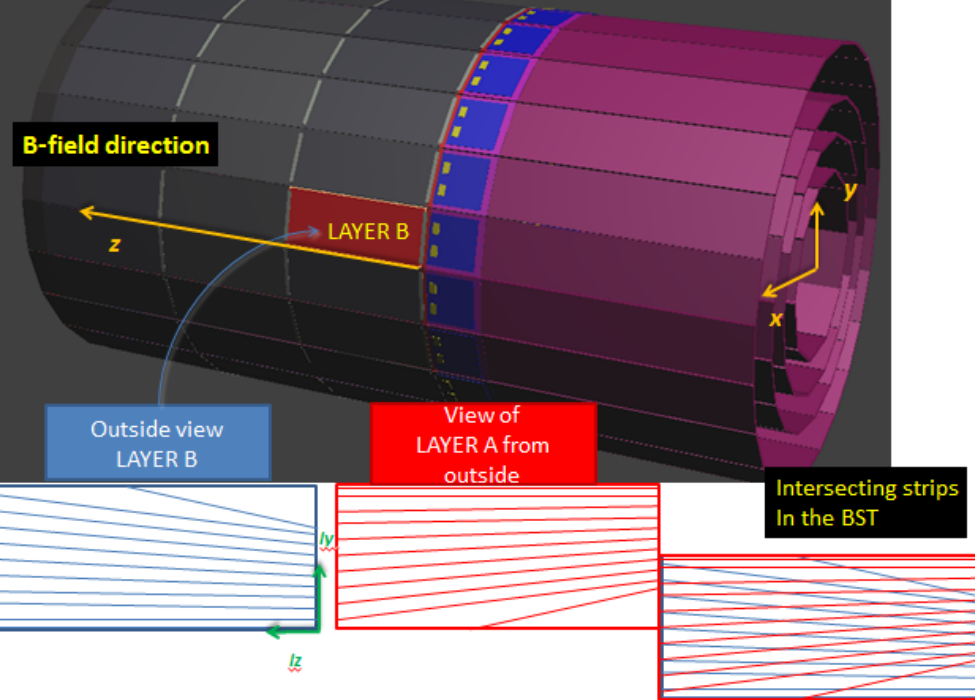
\includegraphics[width=12cm]{CLAS-12/modules/clas-12-system/pics/cd/svt.PNG}
    			\caption{Silicon Vertex Tracker}
			\end{figure}  
			
			
			 \begin{figure}[H]
    			\centering
    			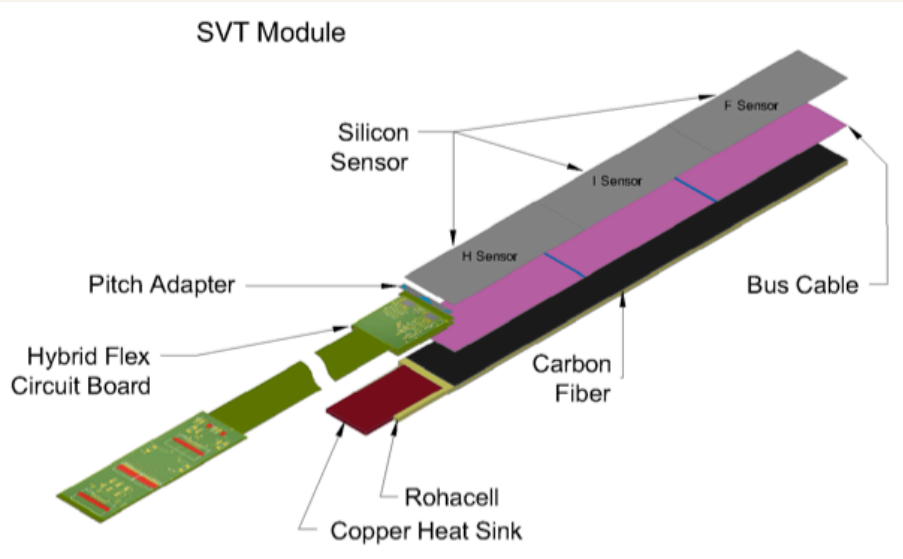
\includegraphics[width=12cm]{CLAS-12/modules/clas-12-system/pics/cd/svt-module.PNG}
    			\caption{SVT Strip}
			\end{figure}  
			
		
		\subsection{MMVT}
		    Composed of two parts: a \textbf{Barrel Tracker} and a \textbf{Forward Tracker}. PCB is 200 $\mu$m thick, 0.3\% of a radiation length. 20 MHz sampling frequency. Time resolution of 10 ns. 500 $\mu$m strip pitch.\\
		    \textbf{Advantages of MMVT for CLAS12 :} \\
		    Price: much cheaper compared to SVT. For large area, the price become rapidly prohibitive.
		    Material: Since it is a gasesous detector, it is good for the material budget.
		    Physics Requirements: Not as good spatial resolution as SVT, but can resolve polar angle better. Optimal perform ace is actually achieved with a combination of both detectors are used.
		    \newline
		    Overall momentum uncertainty ($\sigma_p$/p) = 1.6\%. $\sigma_{\theta}$ = 1.4 mrad.  $\sigma_{\phi}$ = 2.6 mrad.  $\sigma _{z}$ = 270 mm.  
		    \subsubsection{Barrel Tracker}
		        18 cylindrical detectors arranged in 6 layers. Covers 35 to 125 degrees. 15,000 readout elements.Gas Mixture 90\% Argon, 10\% isobutane. 3 mm drift gap. 5 kV/cm field. 75\% mesh transparency.
		    \subsubsection{Forward Tracker}
		        6 circular, flat detectors from 6 to 29 degrees in $\theta$. Improves vertex resolution by a factor of up to 10x compared to just the drift chambers along. 6,000 readout elements. 80\% neon, 10\% ethane, 10\% Carbon Tetrafluoride. 5 mm drift gap. 1kV/cm field. 100\% mesh transparency.
		        
		        
		        						
									
			 \begin{figure}[H]
    			\centering
    			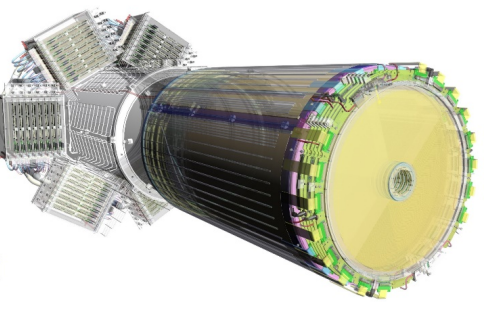
\includegraphics[width=12cm]{CLAS-12/modules/clas-12-system/pics/cd/MVT.PNG}
    			\caption{SVT Strip}
			\end{figure}
 
    
        \subsection{CTOF}
            Central for PID purposes. Divides into 48 1 meter long plastic scintillators with double sided PMT readout.PMTs are in the 0.1 T fringe field region and enclosed in magnetic shielding. 65 picosecond timing resolution. 35 to 125 degrees, 2 $\pi$ in polar angle. 3 cm x 3 cm scintillator planks. Pion/Kaon separation up to 0.64 GeV, Kaon/proton separation up to 1 GeV, pion proton separation up to 1.25 GeV.  
            
            						
			 \begin{figure}[H]
    			\centering
    			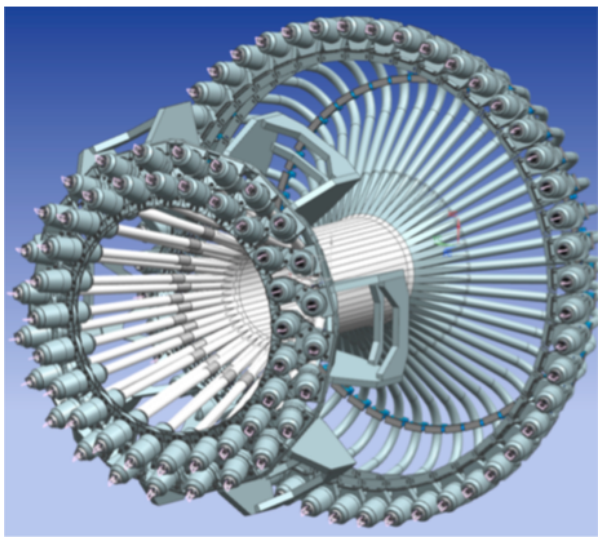
\includegraphics[width=12cm]{CLAS-12/modules/clas-12-system/pics/cd/CTOF.PNG}
    			\caption{SVT Strip}
			\end{figure}
            
 
		\subsection{CND}
		    Detects 0.2-1 GeV neutrons. 3 layers, 48 paddles per layer. Plastic scintillator, 3 cm x 3cm, 0.7 meters  long. Neutron detection efficiency $\sim$ 10\%. 130 picosecond timing resolution, 2 degrees angular resolution (polar and azimuth).
            
            						
			 \begin{figure}[H]
    			\centering
    			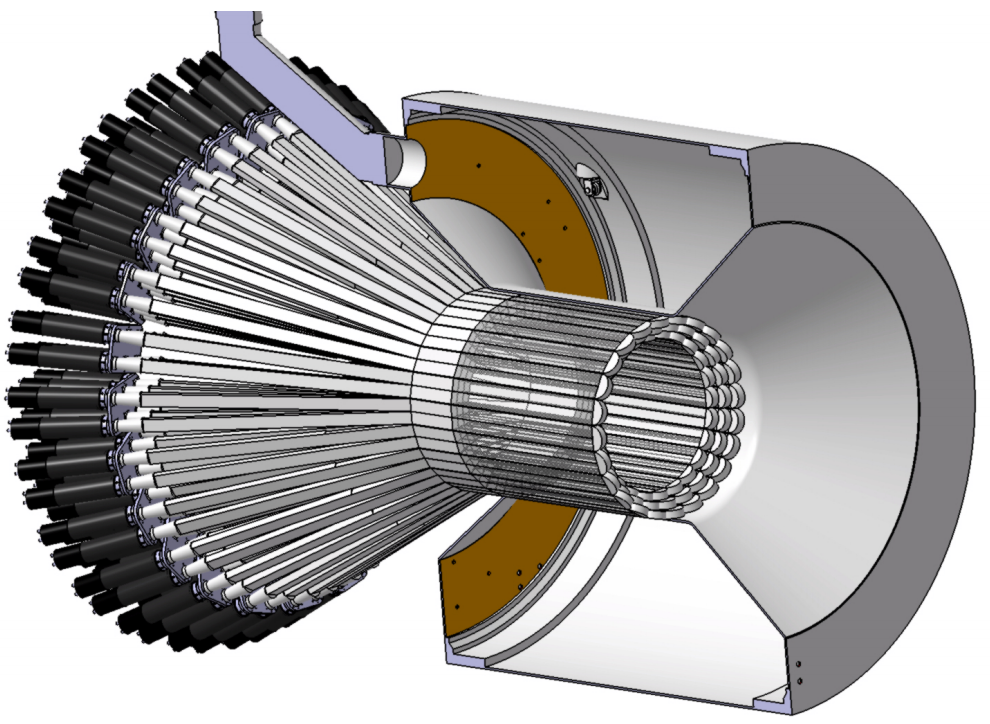
\includegraphics[width=12cm]{CLAS-12/modules/clas-12-system/pics/cd/CND.PNG}
    			\caption{SVT Strip}
			\end{figure} 

		\subsection{Solenoid}
		    5 Tesla super conducting magnet, uniform field ($\Delta$B/B = $10^-4$). Weakest at small angles, strongest at large angles. Opening polar angle of 40 degrees. Momentum range of interest 0.3 to 1.3 GeV. 18 Megajoules stored energy. 85 cm in diameter, 4.2 Kelvin operation. 
		    
    \section{Forward Detector}
        Overview:
        \subsection{HTCC}
            Used basically as an electron trigger. Composed of 60 lightweight ellipsoidal mirrors, that focus Cherenkov light onto eigh 5-inch phototubes (48 channels on entire HTCC). Working gas is CO2 at STP (n=1.0005, $\theta_{max}$ = 1.7 degrees, covers 5 to 35 degrees, 2$\pi$ in azimuth. Active area 2.4 meters in diameter. Electron signal threshold is 15 MeV, charged pion threshold is 5 GeV. 99.9\% electron detection efficiency vs. pions. 15 feet in diameter, 6 feet long. Mirror thickness is 0.1 g/$cm^2$. Kaons have no signal, as they would need 16 GeV to generate a signal. Uses Winston cones to increase collection efficiency. 20 photoelectrons per electron in HTCC, 25\% quantum efficency. The PMTs have 14 dynodes, gain of about $10^7$. HTCC material budget 0.135 g/$cm^2$
            
            									
			 \begin{figure}[H]
    			\centering
    			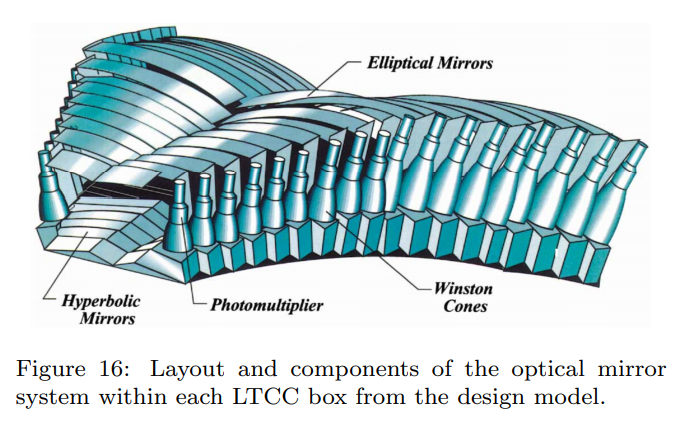
\includegraphics[width=12cm]{CLAS-12/modules/clas-12-system/pics/fd/htcc-mirrors.PNG}
    			\caption{SVT Strip}
			\end{figure}
			
						
									
			 \begin{figure}[H]
    			\centering
    			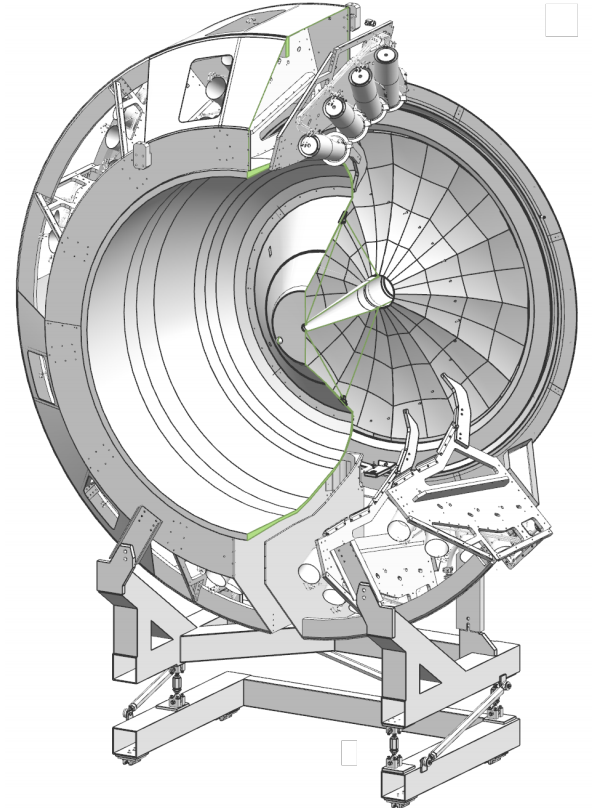
\includegraphics[width=12cm]{CLAS-12/modules/clas-12-system/pics/fd/htcc.PNG}
    			\caption{SVT Strip}
			\end{figure}
			
			

        \subsection{Torus}
            6 coil torus, 4k amps, 3.5 Tesla torodial field, supercritical LHe cooled. 14.2 Megajoules stored energy. 2 Henries of inductance. Field strongest at small angles, weakest at large angles. 
              Inbending vs out bending:
        I have been wondering about this as well. All I know is that inbending and outbending have different acceptances.
        So, I guess some channels prefers inbending while the others do outbending? I’m not sure though. FX claims outbending results have better quality for these days. 
            									
			 \begin{figure}[H]
    			\centering
    			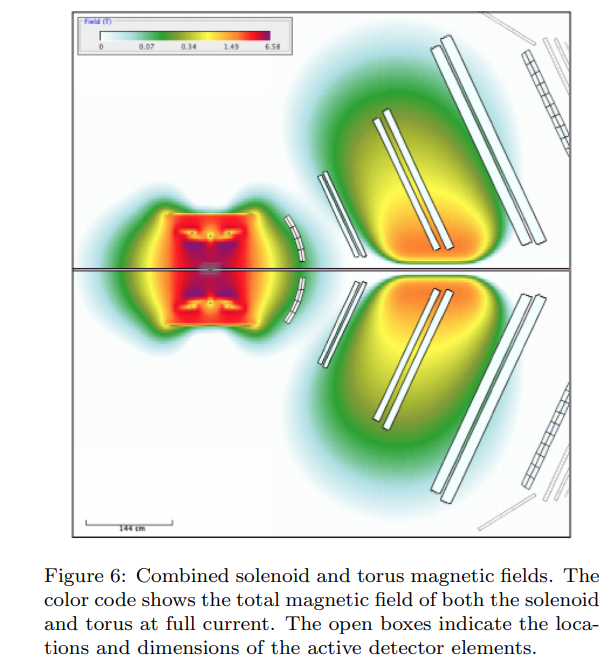
\includegraphics[width=12cm]{CLAS-12/modules/clas-12-system/pics/fd/torus.PNG}
    			\caption{SVT Strip}
			\end{figure}
                        

        \subsection{Drift Chambers}
            There are 3 layers of drift chambers, each with 6 sections. Each chamber has 2 superlayers of 6 layers by 112 wires, for a total of 24,192 wires. (Structure is 112 wires * 6 layers * 2 superlayers * 18 DC sections = 24,192 wires). Physical wire sectioning looks like:\\
            (IIIIII)-(IIIIII)---(IIIIII)-(IIIIII)---(IIIIII)-(IIIIII) x 6 sectors\\
            Where each "I" is a layer of 112 wires.\\
            Spatial resolution is 300 $\mu$ m, angular coverage 5-40 degrees. Momentum resolution $\Delta$p/p < 1\%, angular resolution is 1 mrad in theta, 1mrad/$\sin{\theta}$ for phi. The Drift Chambers are located 2, 3, and 4 meters from the gas mixture is 90/10 Argon/CO2. Time resolution = ?\\
            DC specifics: 30 micron diameter tungsten sense wires, 80 micron Cu-Be field wires, 140 micron Cu-Be guard wires. 20 g tension on sense, 62 g tension of field, 180 g on guard. Max sag calculated to be on order of 10 microns.
            
            									
			 \begin{figure}[H]
    			\centering
    			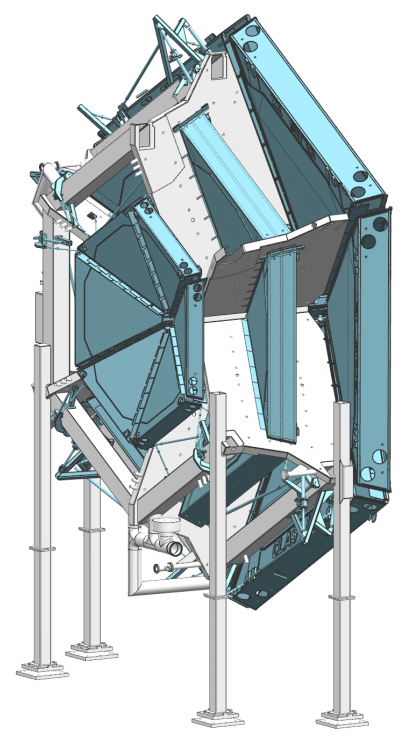
\includegraphics[width=12cm]{CLAS-12/modules/clas-12-system/pics/fd/drift-chambers.PNG}
    			\caption{SVT Strip}
			\end{figure}    

            
        \subsection{LTCC}
            6 sectors, perfluorobutane ($C_4F_10$) $\longrightarrow$ n = 1.0013 $\longrightarrow$ $\theta_{max}$ = 3 degrees. Electron threshold 9 MeV, pion threshold 2.7 GeV, Kaon threshold 9.4 GeV. Allows for good pion/kaon discrimination from 3.5 Gev to 9 GeV. \\
            Each section has 108 mirrors, 36 winston cones, and 36 PMTs. Mirror is aluminium with $MgF_2$ coating. Kevlar support structure. Perflourobutane is 100\% transparent above 220 nm light. 
            
            
						
									
			 \begin{figure}[H]
    			\centering
    			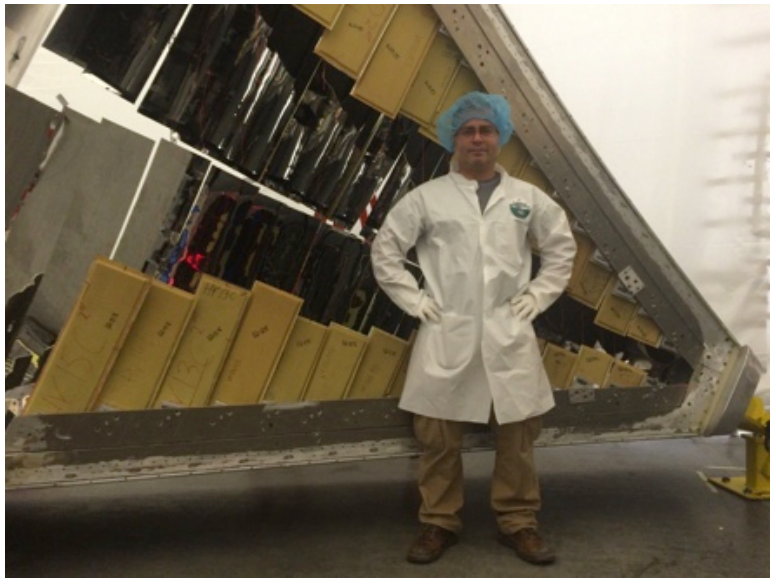
\includegraphics[width=12cm]{CLAS-12/modules/clas-12-system/pics/fd/ltcc.PNG}
    			\caption{Low Threshold Chrenkov Counter}
			\end{figure}
			
			

			
        \subsection{RICH}
            Provides PID in the range of 3-8 GeV, replacing one sector of LTCC (right middle sector). Pion/Kaon rejection factor > 500, Kaon/Proton rejection factor > 100. Covers 5 to 25 degrees in theta, uses aerogel (n=1.05 $\longrightarrow$ $\theta_{max}$ = 18 degrees). Pion threshold 460 MeV, Kaon threshold 1.6 GeV. Read out by 64 channel photomultipliers. $\beta_{min}$=0.95, $\gamma_{min}$ = 3.3
            
            What is angular resolution?
            
            Reminder of relevant equation:
            \begin{equation}
                \cos{\theta} = \frac{1}{\beta n} \longrightarrow \theta = \arccos{\frac{1}{\beta n}}
            \end{equation}
            
            \begin{equation}
                \gamma = \frac{1}{\sqrt{1-\beta^2}} \longrightarrow \beta = 1-\frac{1}{1-\gamma^2} 
            \end{equation}
            
            \begin{table}[H]
                \centering
                    \begin{tabular}{llll}
                         & momentum & $\sim \gamma$ & $\theta$  \\
                    pion & 3        & 21            & 17.4                      \\
                    kaon & 3        & 6             & 12                        \\
                         &          &               &                         \\
                    pion & 5      & 36            & 17.6                      \\
                    kaon & 5       & 10.1             & 15.9                        \\
                         &          &               &                          \\
                    pion & 8      & 57.1            & 17.7                      \\
                    kaon & 8       & 16             & 17.1                        \\
                    
                    \end{tabular}
            \end{table}
            
        
            
            
            
            \begin{table}[H]
                \centering
                    \begin{tabular}{lll}
                        Detector    &   Scintillator                         &   PMT   \\
                        FTOF - 1a   &     \textcolor{blue}{BC-408}           &   \textcolor{red}{Phillips XP2262, EMI 9954A}\\
                        FTOF - 1b   &     \textcolor{red}{BC-404}           &   \textcolor{blue}{Hama. R9779} \\
                        FTOF - 2    &     \textcolor{blue}{BC-408}           &   \textcolor{magenta}{EMI 4312KB} \\
                        PCAL        &     FNAL                               &   \textcolor{red}{Hama. R6095}\\
                        ECAL        &     \textcolor{cyan}{BC-412}           &   \textcolor{red}{Philips XP2262, EMI 9954}\\
                        CND         &     \textcolor{red}{EJ-200}            &   \textcolor{cyan}{Hama. R10533} \\
                        CTOF        &     \textcolor{blue}{BC-408}           &   \textcolor{green}{Hama. R2083} \\
                        HTCC        &         N/A                            &   ET 9823QKB \\
                        LTCC        &           N/A                          &   200 Photonis XP 4500B\\
                        LTCC        &              N/A                       &   16 Photonis XP 4508 (Quartz Window)\\
                    \end{tabular}
            \end{table}
            
            *ET stands for Electron Tube, a company. Could not find a spec sheet for this PMT type. 
            ** Could not find spec sheets for either HTCC, or LTCC PMTs. 
       
               
            \begin{table}[H]
                \centering
                    \begin{tabular}{lllllll}
                        Scintillator                    & Detectors             &   Principal Use/Features      &   L.O. & WME & R/D Time & L.A. Length \\
                         \textcolor{red}{BC-404}       &  FTOF-1b              &   Fast Counting                   &           68    &   408    & 0.7/1.8           &   140   \\
                         \textcolor{blue}{BC-408}       &  FTOF-1b,2,CTOF       &   TOF - Large Area                &           64    &   425   &   0.9/2.1         &   210  \\
                        \textcolor{cyan}{BC-412}        &  ECAL                 &   Large Area                      &           60   &   434 &   1.0/3/3         &   210\\
                        \textcolor{red}{EJ-200}        &  CND                  &   Long attenuation, fast   &           64     &   425       &   0.9/2.1         &   380   \\
                    \end{tabular}
            \end{table}   
            
            L.O - Light Output - \% Anthracene
            WME - Wavelength Maximum of Emitted Photons
            R/D Time - Rise / Decay time (ns)
            L.A. Length - light attenuation length (cm)
             
             All scintillators have a PVT (Polyvinyltoluene) base. 
             
             EJ-200:          200 -- 10K photons per 1 MeV. 
             
             Thermal effects: EJ-200 loses 5\% of its light output between 20 degrees C and 60 degrees C. No change between -60 to 20 degrees C. 
            
            \begin{table}[H]
                \centering
                %\begin{localsize}{10}
                \scalebox{0.9}{
                    \begin{tabular}{llllllll}
                        PMT                                         & Det.                      &       TS/A    &   WVE         &   PHTC    &   DNY     &       Anode  &    Time Resp.\\ 
                        \textcolor{red}{Hama. R6095}               &  PCAL                     &       28/25   &   300/420/650 & BA/BSG & B\&L/11/2.1  &   1500/0.1    & 4/30/3    \\
                        \textcolor{blue}{Hama. R9779}               &  FTOF-1b                  &       51/46   &   300/420/650 & BA/BSG & LF/8/0.5     &   1750 /0.1   & 1.8/20/0.25 \\
                        \textcolor{cyan}{Hama. R10533}              &  CND                      &       51/46   &   300/420/650 & BA/BSG & LF/10/4.2    &   1000/0.1    &  2/24    \\   
                        \textcolor{green}{Hama. R2083}              &  CTOF                     &       51/46   &   300/420/650 & BA BSG & LF/8/2.5     &   3000/0.2    & 0.7/16/    \\
                        \textcolor{red}{Phillips XP2262}            &  FT1a ECAL            &    &&&&&\\
                        \textcolor{red}{EMI 9954A}                  &  FT1a ECAL            &    &&&&&\\
                        \textcolor{magenta}{EMI 4312KB}             &  FTOF-2                   &    &&&&&\\
                    \end{tabular}}
                %\end{localsize}
            \end{table} 
            
            No spec sheets could be found for the PMTs used in the TFOT1a, ECAL, or FTOF-2.
            Typical dark currents for all PMTs are 100 nA. 
        
            
            Tube size / photocathode area (diameter in mm)
            Wavelength short / peak / long (nm)
            Photocathode / window material (BA = Bialkali, BSG = Borosilicate Glass)
            Dynode structure / stages / gain  LF = Linear-focused, B\&L = Box and line / / Gain - Gain x 10$^6$
            Anode to Cathode Voltage / Anode Current  - Volts / mA
            Rise / transit time/time spread in ns
            
            
            
            \href{https://www.hamamatsu.com/eu/en/product/type/R10533/index.html}{R10533 PMT}
            \href{https://www.hamamatsu.com/eu/en/product/type/R2083/index.html}{R2083 PMT}
            \href{https://pdf1.alldatasheet.com/datasheet-pdf/view/212324/HAMAMATSU/R9779.html}{R9779 PMT}
            \href{https://www.sphere.bc.ca/test/phototubes2/ham/r6095.pdf}{R6095 PMT}
            
            
            
            
            
            
            
            
            
            \href{https://eljentechnology.com/products/plastic-scintillators/ej-200-ej-204-ej-208-ej-212}{CND Scintillator}
            
            
            \href{https://www.crystals.saint-gobain.com/sites/imdf.crystals.com/files/documents/bc400-404-408-412-416-data-sheet.pdf}{BC Scint Specs from Saint Gobain}
            
            
            \href{https://www.hamamatsu.com/eu/en/product/type/R10533/index.html}{CND PMT}
            
            
            \href{https://www.hamamatsu.com/us/en/product/type/R2083/index.html}{CTOF PMT Spec sheet}
            Bialkali photocathode, 8 dynodes, 2.5*10$^6$ typical gain
            Linear-focused dynode structure
            Window material Borosilicate glass
            peak wavelength 420 nm, range from 300 to 650 nm. Max anode to cathode voltage of 3500 V, made anode current of 0.2 mA. Dark current around 100 nA. 
            
            
        
        \subsection{FTOF}
            Used for PID, three layer system - 1a, 1b, and 2. Has a design resolution of 60 ps to 160 ps. Average scintillation rate 250 kHz. Pion/Kaon separation up to 2.8 GeV, Kaon Proton separation up to 4.8 GeV, pion proton separation up to 5.4 GeV. \\
            6 meters away from target.
            Time resolution of 80 ps less than 36 degrees, 150 ps greater than 36 degrees. PMTs are shileded from CLAS12 torus. 6 sectors, plastic scintillator, double sided PMT readout. 3 panesl - 1a - 23 counters, 1b - 62 counters, 2 - 5 counters. \\
            15cm wide x 5 cm deep x 33 cm up to 376 cm long.\\
            20-30 cm up to 15x5 130 ps\\
            350-400 cm 6x6 60 ps\\
            370 to 430 cm, 22x5cm, 150 ps\\
            
            									
			 \begin{figure}[H]
    			\centering
    			\includegraphics[width=12cm]{CLAS-12/modules/clas-12-system/pics/fd/ftof-front.PNG}
    			\caption{SVT Strip}
			\end{figure}

		
			 \begin{figure}[H]
    			\centering
    			\includegraphics[width=12cm]{CLAS-12/modules/clas-12-system/pics/fd/clas12-ftof-geom.PNG}
    			\caption{SVT Strip}
			\end{figure}
			
			
            
            The timing resolution minimums are for being close to the beam axis where particles are moving faster, and farther out from the beamline (larger theta) particles are moving slower so a less resolved time difference is acceptable. 
            
            \subsubsection{1a}
                Coverage is 50\% at 5 degrees to 85\% at 35 degrees\\
                Dimensions: L 32.3 cm to 376.1 cm, wxh = 15x5 cm\\
                Material BC-408\\
                PMTS: EMI 9954A, Phillips XP2262\\
                Time resolution 90 - 160 ps small bar to big bars\\
            \subsubsection{1b}
                Coverage is 50\% at 5 degrees to 85\% at 35 degrees\\
                Dimensions: L 17.3 cm to 407.9 cm, wxh = 6x6 cm\\
                Material BC-404 (first half) and BC-408\\
                PMTS: Hamamatsu R9779\\
                Time resolution 60-110 ps small bar to big bars\\
            \subsubsection{2}
                Coverage is 85\% at 35 degrees to 90\% at 45 degrees\\
                Dimensions: L 371.3 cm to 426.2 cm, wxh = 22x5 cm\\
                Material BC-408\\
                PMTS: EEMI 4312KB\\
                Time resolution 140 - 165 ps small bar to big bars\\
           
           
            For more FTOF specifcications, look \href{https://www.jlab.org/Hall-B/ftof/notes/ftof_geom.pdf}{here} 
                
            FTOF two panels:
Official answer from CLAS12 FTOF NIM paper:
"For tracks that pass through both arrays the combined time information (described in Ref. [10]) is used and results in a 20% improvement compared to using the hit information from panel-1b alone.”, https://www.sciencedirect.com/science/article/pii/S0168900220302102

I guess this is the right answer though:
1a is recycled one from CLAS while 1b is new one.
            
            
        \subsection{PCal and ECal}
            ECal from CLAs could only contain showers with E < 5 GeV. Above 5.5 GeV, couldn't resolve neutral pion gamma gamma angle, so needed PCAL. PCAL is 7 meters from target, ECAL is 7.5 M from target. EC segmentation 10 cm, PCAL finer segmentation. PCal 5.5 radiation lengths. 20.5 radiation lengths total. Both are sampling calorimeters, with PB and scintillator layers. The CLAS ECAL was resused and a new PCAL was installed in front of it. Primarily used for identification of electrons, photons, gamma gamma decays from pions, and neutrons. They are sampling calorimeters with six moduels. Each module has a triangular shape with 54 (15/15/24 - PCAL/ECALinner/ECALouter) layers of 1 cm htick scintillators segmented into 4.5/10 cm (PCAL/ECAL) wide strips and sandwiched between 2.2 mm thick lead sheets. The total thickness is about 20.5 radiation lengths. \\
            \indent Scintillator layers are grouped into three readout views with 5/5/8 PCAL/ECinner/ECouter, layers per view providing several cm resolution of energy clusters. Light from each scintillator readout group is routed to PMTs via flexible optical fibers.\\
            Overall perfomance:\\
            Energy resolution of 10\%, position resolution of 2 cm, time resolution of 500 ps. \\
            Are these the real statistics? Because they seem like BS.
            
            
            
            \begin{figure}[H]
    			\centering
    			\includegraphics[width=12cm]{CLAS-12/modules/clas-12-system/pics/fd/sample-BC-408-emission-spectra.PNG}
    			\caption{BC 408 Emission Spectra}
			\end{figure}
			
            						
									
			 \begin{figure}[H]
    			\centering
    			\includegraphics[width=12cm]{CLAS-12/modules/clas-12-system/pics/fd/clas12-pcal-ecal.PNG}
    			\caption{SVT Strip}
			\end{figure}
			
			
            \subsubsection{PCAL}
                \indent 50\% coverage at 5 degrees, 85\% coverage at 35 degrees. 15 scintillators, 14 lead layers, per module. 1200 scintillator strips, 1x4.5 cm$^2$ up to 432 cm long, with two holes along the strip, and 0.25 mm TiO2 coating (reflective coating)\\
                Lead sheets are 2.2 mm thick. Readout by fibers into 1 inch PMTs, Hamamatsu R6095. Light yield is 11-12 photo-electrons per MeV. 
                
                PCAL scinitllator was manufactured at the FNAL-NICADD Extrusion Line Facility. Polystyrene base was Dow STYRON 663 W, primary dopant is 2,5 -diphenyloxazole (PPO, 1\% by weight) - this is the organic scintillator, peaks at 385 nm:
                
                
            \begin{figure}[H]
    			\centering
    			\includegraphics[width=12cm]{CLAS-12/modules/clas-12-system/pics/fd/2-5-diphenyloxazole.png}
    			\caption{2,5-diphenyloxazole}
			\end{figure}
                
                The Secondary dopant is 1,4 bis (5-phenyloxazol- 2-yl) benzene (POPOP, 0.03\% by weight) - also scintillator, peaks at 410 nm. 
                
                                
            \begin{figure}[H]
    			\centering
    			\includegraphics[width=12cm]{CLAS-12/modules/clas-12-system/pics/fd/popop.png}
    			\caption{1,4 bis (5-phenyloxazol- 2-yl) benzene}
			\end{figure}
                
                
                
                A reflective surface coating of polystyrene with 12\% TiO2 with 0.25 mm nominal thickness was co-extruded. 
                
                Cast plastic scintillator costs about \$50 per kg, while extruded scintillator is significantly lower in price - about \$10 per kg. 
                
                \href{https://lss.fnal.gov/archive/2005/pub/fermilab-pub-05-344.pdf}{Interesting write up on FNAL Scintillator extrustion}


\href{https://www.sciencedirect.com/science/article/pii/S0168900220300309?via\%3Dihub}{PCal Technical Report}
\href{https://www.sciencedirect.com/science/article/pii/S0168900200009967}{ECal Technical Report}

                
            \subsubsection{ECAL}
                \indent 50\% coverage at 5 degrees, 85\% coverage at 35 degrees. 39/38 scintillators / lead layers per module. 216 readout channels per module, 1200 strips per module. Strips are 1x10to12cm$^2$ by up to 441 cm long, BC-412 (plastic scintillator with high light output, longest light attentuation length, \href{https://www.crystals.saint-gobain.com/products/bc-408-bc-412-bc-416}{cheap!} ). Lead sheets are 2.4 mm thick. Read out by fiber into 2 inch PMTs, Phillips XP2262 and EMI 9954. 3-4 photoelectrons/MeV deposited energy. 

    


Other:
Forward Tagger, BAND, not important.

20 kHz Level 1 trigger rate, 1 GB/s.

Only about 50\% of the electron triggers recorded with an inbending torus polarity are actually electrons. For outbending torus polarity, hte electron trigger purity is as high at 70\%. 

\href{https://www.jlab.org/Hall-B/clas12-web/}{Detector Specs}



Outbending allows for lower Q2 measurements, inbending allows for slighly higher Q2 measurements. 



By measuring DVMP, we can get information about GPDs in the following way – in the leading twist approximation / some other formalism bullshit, dvmp cross section is described by the generalized Compton form factors, which themselves are (to leading twist etc.) convolutions of GPDs, so the dvmp cross section sets constraints on GPD behavior.

  hard exclusive pseudoscalar meson electroproduction in recent years has shown that the asymptotic leading twist approximation is not readily applicable in the range of kinematics accessible to current experiments. In fact, there are strong contributions from transversely polarized virtual photons that are asymptotically supprsed by $1/@^w$ in the cross sections and have to be considered by introduing chiral-odd GPDs into the framework.   



Hi Bobby, so sorry for late reply I was busy with readiness review preparation.
So Q2>1 is indeed for deeply virtual events, however it has no relation with lepton/hadron angle. There are pi0 events in the region below 1GeV2, and they are also pi0 events. The limit on 1GeV2 is somewhat artificial. Ideally we are looking at the asymptotic freedom, so Q2 should be infinity, but we are hoping that 1GeV2 is big enough to apply models that are based on asymptotic freedom. There are many terms also that are proportional to powers of t/Q2. So we need reasonably big Q2 to apply GPDs models. And in fact CLAS kinematics is often questioned to be too small for GPDs theoretical models.


\chapter{DVEP and GPDs - what are we here for}
    DVMP:

    Deep exclusive processes can allow access to Generalized Parton Distributions (GPDs), a concept that lies at the root of 3D imaging of the proton's quark-gluon substructure, as GPDs contain information about the transverse spatial distribution of quarks and their longitudinal momentum inside hadrons. The key to extracting GPDs from experiments are the Quantum Chromodynamics (QCD) factorization theorems. Deeply Virtual Compton Scattering (DVCS) is the cleanest way to
    
    study GPDs. While DVCS data have given hints of the factorization regime being attained, such hints have not been observed for Deeply Virtual Meson Production (DVMP) data. Exclusive $\pi^0$ electroproduction has been measured by experiment E12-06-114 in Hall A of JLab in order to test factorization in DVMP processes. Cross sections have been measured at three fixed Bjorken- x (xB) : 0.36, 0.48 and 0.6 in the Q2 range 3 to 9 GeV2. High statistical measurements of polarized and unpolarized cross sections of H(e,e',gamms) p could allow mapping and extraction of GPD information from the nucleon. In this talk, I will show the experimental setup, calibration and preliminary results of the neutral pion electroproduction cross sections for xB >0.3 from this experiment.  




    \section{GPDs}
        \subsection{PDFs}
        \subsection{The GTMD Cube}
        \subsection{GPDs and Helicity Odd Structure Functions}
    \section{DVEP}
        \subsection{DVEP, DVCS, and DVMP}
            \subsubsection{DVEP}
            \subsubsection{DVCS}
            \subsubsection{DVMP}
    \subsection{How DVPiP Relates to GPDs}
    \subsection{CLAS12 - DVMP Questions}
        \subsubsection{Intuition about DVMP}

        First, note that not all DVMP reactions are sensitive to nuclear transversity distributions, which involves quark helicity flip of transversely polarized quarks helicity  This can occur in  production of pseudoscaler mesons,  e.g. pi0 and eta production, with spin-charge-parity  I-PC= 0 - + ,in contrast with  the incident photon, which  has J-P 1- -. This is not the case for other mesons studied at JLab, such as vector mesons, I-PC= 0 - e.g. the rho, omega, phi, for which which I-CP= 1- -, the same as for the photons.   I believe this was first  pointed out  Ahmad, Goldstein, Liutti (arXiv:0805.3568). Here is a quote from their intro.
        "... deeply virtual $\pi^0$ (as well as $\eta$, $\eta'$) production off a proton target is clearly distinct from the other types of meson production processes in that it involves the transition of a (virtual) photon with JPC = 1-- to a JPC = 0-+ state (i.e. the final $\pi^0$ or $\eta$, $\eta$') requiring odd C-parity and chiral odd t-channel quantum numbers. As a consequence, in a partonic description such as the one depicted in Fig.1a, the ”outgoing” and ”returning” quark helicities need to be opposite to one another …". 
        
        Peter Kroll, who works very closely this group, with Sergei Goloskokov, Marcus Diehl, et al. have published extensive theoretical calculations based on Jlab data.   Gary Goldstein, Simonetta Liutti have have also published on this  reaction.
        
        By the way, the other meson production channels  are uniquely sensitive to other  interesting aspects of nucleon structure. For example, the phi, on which F-X and Patrick are working, is very sensitive to the gluon distribution in the nucleon.
        
        In DVCS the  incident and  outgoing particles are both photons JP= 1-. Therefore, no quark helicity flip is necessary in this “virtual Compton scattering”.  Therefore DVCS is primarily sensitive to non-quark spin flip - eg. H.. The same is true with DVMP of other vector meson, such as rho.  
    	However,  since the pi0 and eta are JP=0-, then the transverse photon part contributing to the overall reaction cross section can cause a transversely polarized  quark helicity flip. This is contained mainly  in the structure functions $\sigma_T$ and $\sigma_{TT}$, which can be decomposed into the transverity GPDs - mainly $Ebar_T$ and $H_T$. 
    	
    	Also, pion and eta production can still also be accompanied by non-quark helicity flips, which would be mainly contained in the longitudinal structure functions $\sigma_{LL}$. However, various theoretical papers indicate that in our accessible region of $Q^2$, $\sigma_T$ and $\sigma_{TT}$ dominate relative to $\sigma_L$. Experimentally, this seems to be verified from JLab data .
    	On the other hand, theory predicts that asymptotically, $\sigma_L$ will dominate. From our existing 5 GeV  data, we are not anywhere near there, so our experiments at JLab are really just right for accessing these transversity distributions.  But, to decompose these distributions  at the level of the individual quark u d flavors, we need as much precision data over as big a range as possible of kinematics in several channels - P-pi0, N-pi0, P-eta, N-eta. And, only you guys can do that!
    	So, let me know if this makes sense to you. s a bit. 
    	
        \subsubsection{Why is Phi particularly sensitive to the phi distribution?}

        If you look at the proposal you will see the main diagram we are interested in has a pair of gluons from the GPD bag connecting a the hard scattering kernel that comes from the virtual photon fluctuating into a $s\bar{s}$ pair
        
        The process you mention instead has a pair of strange quarks from the GPD bag connecting to the hard scattering kernel directly. 
        
        In practice the two processes happen. From known PDF however the gluon contribution is expected to be significantly larger than the strange quarks contribution. So the intuitive reason would be: the proton has nearly no strangeness but does have a bunch of gluons.
        
        Now it could be that we are wrong and that the proton has more strangeness than what conventional PDF suggest. This could potentially hamper our strategy. However, intrinsic strangeness is in itself a very interesting subject, and if we did come to the conclusion that the proton has more strangeness than is conventionally accepted, then it would be a very important result.
        
        The way I understand why the phi channel probes the gluon GPDs is because the phi meson is a strange-antistrange meson, and so doesn't interact with the up and down quarks that predominantly make up the quark content of the nucleons. This is from the phi cross section proposal: Because of its almost pure $s\bar{s}$ composition $\phi$ production is not affected by scattering from the nucleon’s valence quarks or the light quark sea;
        
        \subsubsection{How to probe TMDS?}
        About probing TMDs, do you know exactly which groups or what channels can be used to do this at CLAS12? For example, we probe GPDs with DVCS or DVMP. Is there a similar channel that allows access to TMDs?
        
        For first one, look for SIDIS, but I'm not sure about specific channels. I could find slides at
        $https://indico.cern.ch/event/568360/contributions/2487494/attachments/1438684/2213587/PuckettDIS2017.pdf$ from google, but there could be better references. I think I have seen one from collaboration meeting but I'm my way back from Chicago to Boston. You can find whole collaboration meeting slides at $https://www.jlab.org/indico/event/343/other-view?view=standard$

        \subsubsection{FIGURE OUT STT SLT SLL – maybe ask Paul Stoler for more information about this }
\chapter{Thesis Goal}
    \section{What do we want at the end of the day and why?}
    What is the Hall A DVMP measurement?
    gravitational form factor of the proton
    Why is CLAS12 particularly suited for this measurement
    Compare to other experiemnts - hall A, compass, etc. 
    Precision estimate – 10\%? 5\% if we are lucky? What was precision of CLAS6?
    other note – intution for process – not just getting longitudinal momentum information as with DIS, but also get the other piece of information from having put back together the proton. Read about Compton Form Factors/ extensions of. 
    of all electrons that enter target, how many colissions do we get? probably either 1 or none? what is the probability of 1?
    
    Very important and good stating place - write up notes from 2011 pi0 analysis note
    
    Write to Axel at BIn Volume correction, page 75 analysis note fig 6.1
    
    Compare integrated luminosity of CLAS6 to CLAS12 (in 2011 analysis note)
    
    $pi^0 \longrightarrow \gamma \gamma$ branching ratio = 98.8\%
    
    Given we have an interaction, how many do we detect (ep)?
    
    Question: WHy is beam charge important?
    Answer (Brandon Clary, email) The accumulated beam charge is charge measured at the Faraday cup. It's important for determining the luminosity for a run, and even being able to compare data from run to run, especially when runs may have different beam current, for example. It's just a good way to normalize to the total number of electron in that run, file, etc. In principle you could normalize by minutes, hours, etc. But beam charge, number of el., is needed to calculate the luminosity for a fixed target experiment when extracting cross sections.
\chapter{Analysis Scheme}
    \section{Preliminary Plots}
    What is event rate? In Hz or in barns. What is your luminosity?
    Diff between Fast MC and GEMC?
        \subsection{Basic Kinematics}
        \subsection{DVPP Kinematics}

    \section{Technical Details}
        Read about kinematic fitting
            \subsection{Groovy, Python, g/Root, and more}
            
            
            


Low t-data are very important for the meson exclusive physics. The GPD interpretation works only in the region -t/Q2<1. From this point of view the central detector will not only  increase the total statistics by a factor more than 2 but will add the valuable data with low t.


 However, for pi0 the only data we have from Hall A are of very limited statistics and kinematics. One of their limitations was the relatively modest variation on polarization parameter (epsilon) since the beam energies we not so far apart. 
 
 Number of final events in CLAS6 DVMP? About 100K, maybe 200K. 
 
 
 
 Dear Valery

CLAS12 acceptances and resolutions are also superior to that of CLAS6. Main differences are:
- RGK has outbending torus vs inbending CLAS6 data
- the distance between the target and the PCal has increased, the FTCal extends to lower angles, and the gap between FTCal and PCal is much smaller than between IC and EC
- proton polar angle was limited to 60 deg in the e1dvcs dataset if my memory is correct

Do you have on hands the number of exclusive pi0 events published for the CLAS6 cross-sections?
We need numbers to make the case to cook the RGK data

Well over an order of magnitude more statistics at CLAS12 compared to CLAS6


\section{Proton Spin Puzzle}
    Puzzle Origin: How is quark contribution to proton spin measured?
    \subsection{Puzzle Origin}
        Do DIS with a polarized lepton on a polarized proton. The trick is to polarize the proton target in both directions, i.e. run the experiment with the target spin up and again with target spin down. Then measure the asymmetry of the scattered leptons. The EMC collaboration did this with a polarized muon simultaneously on two separate targets with opposite-sign spin. Paper is \href{https://www-sciencedirect-com.libproxy.mit.edu/science/article/pii/0550321389900898?via\%3Dihub}{Here}. To measure the spin contribution of the gluons, you collide two proton beams, first with the spins aligned and then anti-aligned. This was done at RHIC a few years back (relative to 2020). 


            
            
            
            
            
    


\chapter{Experimental Setup} \label{Chapter:Experiment}
   The CLAS12 detector is a large angle spectrometer that generally covers angles from 5 to 130 degrees, spanned by two main detector subsystems - the Forward Detector and the Central Detector.

    Overview of Jefferson Lab
    Why is CLAS12 particularly suited for this measurement?

\section{Accelerator and Beamline}
    The Thomas Jefferson National Accelerator Facility, also called Jefferson Lab (JLab), is one of the 17 National Laboratories in the United States \parencite{DepartmentofEnergy2023DepartmentLaboratories}, and functions mainly to deliver high energy, continuous wave (CW) electron beams to fixed-target nuclear and particle physics experiments. The facility was established in 1984 - initially named the Continuous Electron Beam Accelerator Facility (CEBAF) - and first delivered a 4 GeV electron beam on July 1 1994 to one of its three original detector halls. In 2006 efforts began to upgrade the facility to produce an electron beam up to 12 GeV in energy, which was first successfully delivered in 2015, as well as to construct a fourth detector hall for additional physics experiments\parencite{JeffersonLab2023AboutLab}. JLab is also home to a free-electron laser, capable of 10+ kW CW operation \parencite{Benson2007HighAccelerator}. 

\begin{figure}[ht]
    \centering
    \includegraphics[width=0.8\textwidth]{Chapters/Ch2-Experiment/accel_and_beamline/pics/CEBAF/jlab_wiki.png}
    \caption{An aerial view of the Thomas Jefferson National Accelerator Facility \parencite{Wang2010CEBAFOverview}. Note that this picture was taken before the addition of the fourth detector hall (Hall D).}
    \label{fig:jlab_wiki}
\end{figure}

\subsection{Accelerator Facility}
    
    \figref{fig:jlab_accelerator_layout} shows the overarching scheme of the entire accelerator facility relevant for this experiment. Electrons are produced via the photoelectric effect from a 499 MHz pulsed laser impinges on a Gallium Arsenide photocathode (\figref{fig:gun}). The CEBAF guns operate at 100 kV and accelerate the electrons through a beam chopper (\figref{fig:chopper}) to create the desired beam structure (\figref{fig:structure}) and into the main accelerator circuit, where 1497 MHz superconducting resonator (SRF) cavities provide further acceleration (\figref{fig:klystron}). CEBAF's two $\sim$ 1.1 GV linacs accelerate electrons by consist of 50 cryomodules total, with each cryomodule housing 8 7-cell SRF cavities and the liquid helium necessary to cool them, made possible by JLab's 2K liquid helium refrigerator, the largest in the world as of 2023. The electrons are steered around the curved parts of the track by dipole magnets (\figref{fig:magnets}), making five complete circulations before delivery to the three western experimental halls.
    
    
    \begin{figure}[ht]
        \centering
        \includegraphics[width=0.8\textwidth]{Chapters/Ch2-Experiment/accel_and_beamline/pics/CEBAF/jlab-accelerator-layout.png}
        \caption{Schematic layout of the CEBAF accelerator at JLab. The racetrack configuration has two linear accelerator portions $\sim$ 1/4 mile long, and is $\sim$ 7/8 mile around \parencite{Wang2010CEBAFOverview}.}
        \label{fig:jlab_accelerator_layout}
    \end{figure}
    
    
    \begin{figure}[htb]
        \begin{minipage}[c]{\linewidth}
            \centering
            \subfloat[]{\label{fig:gun}\includegraphics[width=0.3\textwidth]{Chapters/Ch2-Experiment/accel_and_beamline/pics/CEBAF/1_CEBAF-guns.png}}
            \subfloat[]{\label{fig:chopper}\includegraphics[width=0.3\textwidth]{Chapters/Ch2-Experiment/accel_and_beamline/pics/CEBAF/jlab-chopper.png}}
            \subfloat[]{\label{fig:structure}\includegraphics[width=0.3\textwidth]{Chapters/Ch2-Experiment/accel_and_beamline/pics/CEBAF/Jlab-beam-structure.png}}
        \end{minipage}
        \begin{minipage}[c]{\linewidth}
            \centering
            \subfloat[]{\label{fig:klystron}\includegraphics[width=0.4\textwidth]{Chapters/Ch2-Experiment/accel_and_beamline/pics/CEBAF/klystron.png}}
            \subfloat[]{\label{fig:magnets}\includegraphics[width=0.4\textwidth]{Chapters/Ch2-Experiment/accel_and_beamline/pics/CEBAF/magnets2.png}}
        \end{minipage}
        \caption{(a) CEBAF guns, (b) Beam chopper, (c) Beam structure, (d) Superconducting resonator, (e) Dipole magnets.}
        \label{fig:JLab}
    \end{figure}
    

\subsection{Hall B Beamline}

    Moller polarimeters
    raster and target
    faraday cup / beamdump

    
    Finally, excess beam is safely managed using beam dumps. 
    
    \begin{figure}[ht]
        \centering
        \includegraphics[width=0.8\textwidth]{Chapters/Ch2-Experiment/accel_and_beamline/pics/hallB/beamdump1.png}
        \caption{The first stage of the beam dump system at JLab.}
        \label{fig:beam_dump1}
    \end{figure}
    
    \begin{figure}[ht]
        \centering
        \includegraphics[width=0.8\textwidth]{Chapters/Ch2-Experiment/accel_and_beamline/pics/hallB/hall-b-poll-2.jpg}
        \caption{Moller polarimeters}
        \label{fig:beam_dump1}
    \end{figure}

    
    \begin{figure}[ht]
        \centering
        \includegraphics[width=0.8\textwidth]{Chapters/Ch2-Experiment/accel_and_beamline/pics/hallB/beam_rastering.png}
        \caption{The second stage of the beam dump system at JLab.}
        \label{fig:rastering}
    \end{figure}
    
    
    
        in beam dump area, link to own fraday cup paper \cite{Johnston2019RealizationElectrons}
        
    
    For entry into CLAS12, the beamline specs are as follows:\\
                        Beam current: up to 50 nA\\
                        Beam energy spread: $10^-4$\\
                        Beam size: Less than 0.4 mm\\
                        Beam stability: Less than 0.1 mm\\
                        Beam halo: $10^-4$\\
                        Beam polarization: up to 85\%\\
                        
    
    
    
    
    
     As stated, for RGA, the fact that the beam is polarized is not useful, but it is true and is measured by Moller Polarimeters. 
            
                Polarimietry: 
                        Good for beam energies between 100 MeV and 50 GeV. Polarized beam electrons are scat-
                tered from other polarized electrons in a target, usually magnetized foils. Only a small
                fraction of all the target electrons are polarized, so this method has a small analyzing
                power. Analyzing power is exactly calculable in QED. At high beam energies, analyzing
                power and scattering probability both become independently of beam energy. Maximum
                analyzing power is about 80%, maximum is at 90 degrees scattering angle in C.o.M. Trans-
                versely polarized target can be used to measure transverse beam polarization, but analyzing
                power is only about 10%. 90 degrees C.o.M. translates to a small lab angle with each elec-
                tron at half beam energy, so magnets are used to bend these electrons out to detectors.
                These detectors can be, for example lead glass total absorption cherenkov counters.Since
                the two electrons are corellated, can use things like time coincidence to reduce background,
                although for low duty factor accelerators only one electron is required as statistics would
                otherwise be too low.A main background to this process is Mott scattering with the electron
                radiating off energy after scattering, appearing as a Moller electron
                
                The scattering target is either iron or vanadium permendur (iron-cobalt alloy). Only 2 of
                26 electrons in iron have their spins oriented, leading to a total analyzing power of only 6 percent
                and transverse analyzing power of only 1%. Uncertainties in how magnetized the targets
                actually are corresponds to an uncertainty in analyzing power. There are ’easy’ and ’hard’
                magnetization schemes - easy does a soft magnetization, while hard uses a several tesla mag-
                net to saturate the target. In principle, uncertainties on magnetization in the hard scheme
                can be removed by using the Kerr magneto-optic effect, but this has not ever been imple-
                mented. An important correction is due to the Levchuk effect, where due to momentum
                differences between electrons in different shells, electrons scattered off of polarized electrons
                are more likely to be detected than off of unpolarized electrons. Specifically, inner electrons
                are unpolarized and have a large average momenta, so when struck they can fall outside the
                113 TOC
                acceptance of the Moller detectors, while the outer electrons, which are polarized, have a
                small average momentum, and behave as expected. This is up to a 15% effect on polarization
                measurements, and is currently a work in progress.
    
    
                
    
                 Rasterization of some kind
                    \\
                    \indent The hydrogen target in RGA is cooled to 20 K using a He4 evaporation fridge. Can by polarized by dynamic nuclear polarization, driven by a 140 GHz microwave source, can reach 90\% polarization for protons, 40\% for deuterons (both longitudinally polarized). The polarization can be measured by a Q-meter based NMR. 2.5 cm diameter target, extended 5 cm long. \\
                    \indent RGA does not use a polarized target. The beam is polarized, but the target is not, so polarization is not helpful for extracting the 5-fold differential cross section (but it would be if the target was also polarized, and is useful for BSA measurements).
                
       
                Luminosity in CLAS12 is measured from the Faraday Cup and using reference reactions such as elastic scattering. We don't use the Faraday Cup event by event, but we do use it run by run. For beam current measurements, beam position monitors upstream are used - but this is for monitoring on-line, not for analysis.
                           Can manage 175 Watts - 17 nA at 10 GeV. Is used to calibrate beam current, needs a blocker in at higher currents

\cleardoublepage
                                         

\section{CLAS Detectors and Run Conditions}\label{sec:clas12exp}
    The CEBAF Large Acceptance Spectrometer, 12 GeV (CLAS12) detector occupies experimental Hall B at Jefferson Lab. It is an upgrade from its predecessor, the CLAS detector \parencite{Mecking2003TheCLAS}, which operated in the 2000s during the 6 GeV era of JLab and laid the groundwork for the present detector system, which was commissioned in 2018. It covers nearly 4$\pi$ around the target cell, with comprehensive packages of detectors for particle position and energy tracking. It operates with data rates of comparable size to other large-scale, international physics experiments, as shown in \tabref{table:experiments}. Data taking began in 2018 and has an experimental program approved into at least the early 2030s \parencite{Battaglieri2021PresentProgram}.

\iffalse
%Differences between clas and clas12 detectors
CLAS12 acceptances and resolutions are also superior to that of CLAS6. Main differences are:
- RGK has outbending torus vs inbending CLAS6 data
- the distance between the target and the PCal has increased, the FTCal extends to lower angles, and the gap between FTCal and PCal is much smaller than between IC and EC
- proton polar angle was limited to 60 deg in the e1dvcs dataset if my memory is correct
\fi


\begin{table}[h]
    \centering
    \begin{tabular}{l|lccc}
         \headercell{\textbf{Facility}} & \textbf{Experiment} &  \headercell{\textbf{Event Size} \\ \textbf{(kB)}}  &  \headercell{\textbf{L1 Trigger Rate} \\ \textbf{(kHz)}}  &  \headercell{\textbf{Bandwidth to Storage} \\ \textbf{(MB/s)}}      \\ \\ \hline
        JLab & GlueX & 15 & 200 & 300 \\
        JLab & \textcolor{purple}{\textbf{CLAS12}} & \textcolor{purple}{\textbf{20}} & \textcolor{purple}{\textbf{10}} & \textcolor{purple}{\textbf{100}} \\
        LHC & ALICE & 2,500 & 200 & 200 \\
        LHC & ATLAS & 1,500 & 75 & 300 \\
        LHC & CMS & 1,000 & 100 & 100 \\
        LHC & LHCb & 40 & 1,000 & 100 \\
        BNL & STAR & 1,000 & 0.6 & 450 \\
        BNL & PHENIX & 60 & 15 & 450 \\
    \end{tabular}
\caption[Data rates of various physics experiments]{Assorted physics experiments and their typical data rates. Note that exact figures vary by source and run conditions. Adapted from \parencite{DavidLawrence2012TheLab}.}
\label{table:experiments}
\end{table}

\subsection{CLAS12 Detector System}
    The CLAS12 detector \figref{fig:clas12photo} has two major subsystems: the Forward Detector and the Central Detector, as well as a forward tagger (nested inside the forward detector package) and backward angle neutron detector (BAND). 



\begin{figure}[H]
    \centering
    \subfloat[CLAS12 CAD layout.]{\includegraphics[width=0.45\textwidth]{Chapters/Ch2-Experiment/clas-12-exp/clas-detectors/other/pics/CLAS12.png}\label{fig:clas12}}
    \hfill
    \subfloat[CLAS12, fully installed.]{\includegraphics[width=0.45\textwidth]{Chapters/Ch2-Experiment/clas-12-exp/clas-detectors/other/pics/clas-real.png}\label{fig:clas12spec}}
    \caption[CLAS12 Layout]{CLAS12 layout schematic and photograph, from \parencite{Burkert2020TheLaboratory}.}\label{fig:clas12photo}
\end{figure}



\subsubsection*{Forward Detector}

    The Forward Detector (FD) is a 6-fold azimuthally symmetric segmented system containing several detector packages and a toroidal magnet. The sections follow a counterclockwise numbering convention where S1 corresponds to $[-30^{\circ}, 30^{\circ}]$, as in \figref{fig:fd_sections}. Working from the target downstream, the FD consists of a High Threshold Cherenkov Counter (HTCC) \parencite{Sharabian2020TheCounter}, Low Threshold Cherenkov Counter (LTCC) \parencite{Ungaro2020TheDetector}, the Ring Imaging Cherenkov detector (RICH) \parencite{Contalbrigo2020TheDetector}, Forward Time-of-Flight (FTOF) \parencite{Carman2020TheSystem}, Drift Chambers (DC) \parencite{Mestayer2020TheSystem} embedded in a 3.5 Tesla torodial magnetic field \parencite{Fair2020TheMagnets}, and Electromagnetic Calorimeter (ECal) complex \parencite{Asryan2020TheCalorimeter}.

    The ECal consists of three layers, two of which are from the previous CLAS experiment \parencite{Amarian2001TheCalorimeter}. Those two layers were only sufficient to contain showers with energies below 5 GeV, so a third layer (Pre-shower Calorimeter, PCal) was added to address this issue, as well as introduce the finer grained segmentation necessary to resolve the angle between the two photons of a neutral pion decay, which is of special importance for this process measurement. The FD system covers approximately $5^{\circ}$ to $35^{\circ}$ in polar angle, with one layer of the FTOF (FTOF-2) extending coverage to $45^{\circ}$. 
    
    %Likewise, the FTOF has three layers---FTOF 1a, FTOF 1b, and FTOF 2. The LTCC and the RICH were not used in this measurement.
               
    \begin{figure}[H]
        \centering
        \subfloat[FD sectioning.]{
            \includegraphics[width=0.3\textwidth]{Chapters/Ch2-Experiment/clas-12-exp/clas-detectors/fd/pics/ftof-front.png}\label{fig:fd_sections}
        }
        \hfill
        \subfloat[Model of HTCC.]{
            \includegraphics[width=0.3\textwidth]{Chapters/Ch2-Experiment/clas-12-exp/clas-detectors/fd/pics/htcc.png}\label{fig:htcc}
        }
        \hfill
         \subfloat[PCal and ECal assembly.]{
            \includegraphics[width=0.3\textwidth]{Chapters/Ch2-Experiment/clas-12-exp/clas-detectors/fd/pics/clas12-pcal-ecal.png}\label{fig:pcalecal}
        }
        \caption[Forward Detector Packages]{The FD is broken into six sections (a), with the exception of the first component after the target, the HTCC (b). The PCal was added to the ECal from the CLAS experiment to achieve the necessary particle resolution. From \parencite{Burkert2020TheLaboratory}}
        \label{fig:select_FD_components}
    \end{figure}




\subsubsection*{Central Detector}

    The Central Detector (CD) also provides nearly 2$\pi$ azimuthal coverage, and spans from $\sim$ $35^{\circ}$  to $125^{\circ}$ in polar angle. The CD is an approximately 1 meter long cylinder inside a 5 Tesla solenoidal magnet \parencite{Fair2020TheMagnets} with four sub-detector packages. From the target working out, the packages are a Central Vertex Tracker \figref{fig:mvt}, made of a Barrel Micromegas Tracker (BMT) \parencite{Acker2020TheTracker} and Silicon Vertex Tracker (SVT) \parencite{Antonioli2020TheTracker}, a Central Time-of-Flight (CTOF) \parencite{Carman2020TheSystem} \ref{fig:ctof}, and a Central Neutron Detector (CND) \parencite{Chatagnon2020TheDetector}, which was installed but not used in this measurement. 
    
    %The main part is the SVT, while the BMT is used to improve the track reconstruction. 

    Low momentum transfer t \eqref{eq:t_momentum_trans} events correspond to large proton polar angles, meaning the majority of low-t events occur with a proton detected in the CD. These events are important as the GPD interpretation of deeply virtual processes is only valid in the regime where $\frac{-t}{Q^2}$ is small, and as such the CD is invaluable to acquiring data to gain insight on these distributions.        


        %CTOF
        %    Central for PID purposes. Divides into 48 1 meter long plastic scintillators with double sided PMT readout.PMTs are in the 0.1 T fringe field region and enclosed in magnetic shielding. 65 picosecond timing resolution. 35 to 125 degrees, 2 $\pi$ in polar angle. 3 cm x 3 cm scintillator planks. Pion/Kaon separation up to 0.64 GeV, Kaon/proton separation up to 1 GeV, pion proton separation up to 1.25 GeV.  	

 
        
        %Solenoid
	%	    5 Tesla super conducting magnet, uniform field ($\Delta$B/B = $10^-4$). Weakest at small angles, strongest at large angles. Opening polar angle of 40 degrees. Momentum range of interest 0.3 to 1.3 GeV. 18 Megajoules stored energy. 85 cm in diameter, 4.2 Kelvin operation. 


        \begin{figure}[H]
            \centering
            \subfloat[Model of CTOF.]{
                \includegraphics[width=0.3\textwidth]{Chapters/Ch2-Experiment/clas-12-exp/clas-detectors/cd/pics/CTOF.png}\label{fig:ctof}
            }
            \hfill
            \subfloat[Schematic of CVT.]{
                \includegraphics[width=0.3\textwidth]{Chapters/Ch2-Experiment/clas-12-exp/clas-detectors/cd/pics/CVT.png}\label{fig:mvt}
            }
            \hfill
            \subfloat[The CD, in retracted position for maintenance.]{
                \includegraphics[trim={0 5cm 0 0},clip,width=0.3\textwidth]{Chapters/Ch2-Experiment/clas-12-exp/clas-detectors/cd/pics/real_CD.png}
            }
            \caption[Central Detector Packages]{Models of the CTOF (a) and CVT (b) and their physical realizations in the CD (c). Note the first three inner cylindrical layers of the CVT (b) correspond to the SVT, the outer six to the BMT, and the right end cap six to the FMT. Images from \parencite{Burkert2020TheLaboratory}.}
            \label{fig:your_labels}
        \end{figure}
     
        

\subsubsection*{Other System Components}

    At very low beam angles ($2.5^{\circ}$-$4.5^{\circ}$) there is the Forward Tagger (FT) \parencite{Acker2020TheTagger} which contains a tracker, homogeneous calorimeter, and hodoscope. At the other end of the beamline ($155^{\circ}$-$175^{\circ}$) there is the Backward Angle Neutron Detector (BAND)  \parencite{Segarra2020TheBAND}, which is not relevant for this analysis. Furthermore, the BAND and the Forward Micromegas Tracker (FMT)  \parencite{Acker2020TheTracker} were not installed at the time the data for this analysis was taken, although they have since been commissioned. 
    
    

\iffalse
%To possibly encorporate

    \begin{figure}[H]
        \centering
        \subfloat[]{
            \includegraphics[width=0.3\textwidth]{Chapters/Ch2-Experiment/clas-12-exp/clas-detectors/other/pics/clas12-params.png}
        }
        \hfill
        \subfloat[]{
            \includegraphics[width=0.3\textwidth]{Chapters/Ch2-Experiment/clas-12-exp/clas-detectors/other/pics/pid-clas12.png}
        }
        \hfill
        \subfloat[]{
            \includegraphics[width=0.3\textwidth]{Chapters/Ch2-Experiment/clas-12-exp/clas-detectors/other/pics/specs-v2-clas12.png}
        }
        \caption{Your caption goes here}
        \label{fig:others}
    \end{figure}

    
    %From sangbaek
    The Data Acquisition (DAQ) \parencite{Boyarinov2020TheSystem} dead-time can be corrected by using a gate at the FC that closes when the DAQ procedure is complete \parencite{Baltzell2020ThePerformance}. The total charge regardless of the gate is called the ungated charge, and the charge collected during the gate on is the gated charge. The ratio of the gated charge to the ungated charge is recorded as the DAQ live-time. The complete listing of detector components can be found in Table. 2.1. The CLAS12 detector components relevant to the particle 4-momentum vector reconstruction are grouped by their characteristics in Table. 2.2. The essential properties like threshold and resolutions and the prominent material components are also listed. 



    Table 2.2: The properties of the relevant subdetectors for the DVCS analysis. The
    properties relate mostly to the effective measurement uncertainties listed in each NIM
    article [135, 136, 140, 141, 143, 144, 147, 152].
    
    \begin{table}[ht]
        \centering
        \begin{tabularx}{\textwidth}{XccXX}
        \toprule
        Name & Coverage ($^\circ$) & Nominal Property & Material \\
        \midrule
        HTCC & 5-35 & $0.015 < p < 4.9$ GeV/c & CO$_2$ \\
        FTOF 1B & 5-35 & $60 - 110$ ps (t) & \\
        FTOF 1A & 5-35 & $90 - 180$ ps (t) & Plastic \\
        FTOF 2 & 35-45 & $170 - 180$ ps (t) & Scintillator \\
        CTOF & 35-125 & $80$ ps (t) & \\
        ECAL & 5-35 & $10\%/\sqrt{E}$ (E) & Pb (absorber) \\
        & & $1.2$ mrad ($\theta, \phi$) & Plastic scintillator \\
        FT-Cal & 2.5-4.5 & $2\%/\sqrt{E} \oplus 1\%$ (E) & PbWO$_4$ crystal \\
        & & $1.5\%$ ($\theta$) & \\
        & & $2^\circ$ ($\phi$) & \\
        DC & 5-40 & $1\%$ (p) & Aluminium wire \\
        & & $1$ mrad ($\theta$) & $90\%$ Ar \\
        & & $1$ mrad/sin $\theta$ ($\phi$) & $10\%$ CO$_2$ \\
        CVT & 35-125 & $5\%$ ($p_t$) & SVT: Si \\
        & & $10 - 20$ mrad ($\theta$) & BMT: $90\%$Ar + $10\%$C$_4$H$_{10}$ \\
        & & $5$ mrad ($\phi$) & \\
        FC & - & $0.48\%$ (L) & Pb \\
        \bottomrule
        \end{tabularx}
        \caption{Caption}
        \label{tab:my_label}
    \end{table}


\fi


    
\subsection{Experiment Run Conditions}
    
The 499 MHz beam structure equates to a signal with a period of 2.004 ns. In practice, the beam was delivered in every other RF bucket, and so bunched at a period of 4.008 ns.

       
            CLAS12 runs with "open trigger", which means different sub-experiments can define their own triggering logic. There is a standard electron trigger, based off of hits in HTCC, ECal, and FTOF. 

        Only about 50\% of the electron triggers recorded with an inbending torus polarity are actually electrons. For outbending torus polarity, hte electron trigger purity is as high at 70\%. 
    
    \href{https://www.jlab.org/Hall-B/clas12-web/}{Detector Specs}
    
    20 kHz Level 1 trigger rate, 1 GB/s.

   The CLAS12 detector is a large angle spectrometer that generally covers angles from 5 to 130 degrees, spanned by two main detector subsystems - the Forward Detector and the Central Detector.

    
   CLAS12 at the design luminosity of 1035 cm−2 s−1

        Data taken is RGA taken in Fall 2018

        Mention configurations and combinatorics


%from sangbaek
In fall 2018, two sets of experiments have been performed with opposite toroidal magnetic field directions
keeping the other detector settings the same. The toroidal magnet bends the scattered
trigger electron inward or outward along the beam direction. In convention, the torus
polarity associated with the inwardly bending electrons is called the negative, -1,
-100\%, or inbending polarity. The opposite is called the positive, +1, +100\%, or
outbending polarity. Both experiments took data with the beam energy of 10.6 GeV,
and the beam current of about 50 nA. The effects due to the variation in the beam
current during the run periods will be taken into account at the end of the analysis.
The CLAS collaboration performed other CLAS12 experiments with different targets
like liquid deuterium, and various beam energies. The description in this thesis
will be focused on the RG-A fall 2018.

The measured
electron beam polarization was 86.9\% during the RG-A data taking in fall 2018.



\section{Reconstruction and Particle Identification}
    here we talk about CLAS PID
\subsection{Decoding and Track Reconstruction}\label{sec:decrec}

\subsection{Particle Identification}


For this analysis all final state particles should be detected.
After $\pi^0$ decay we are going to have 4 particles: electron, proton and two photons.
The particle identification methods are applied to select the exclusive event with at least one electron, proton and two photons. 


    \subsubsection{Electron}
    \subsubsection{Proton}
    \subsubsection{Photon}
    \subsubsection{Pion}
    
    Basic event builder cuts are utilized, then additional cuts are made that are common with the RGA Analysis note (\href{https://www.overleaf.com/project/5ea737720942930001ff5e9c}{overleaf link} and developed by Sangbaek Lee (sangbaek@mit.edu - \href{https://github.com/Sangbaek/analysis_code/tree/analysis/pid}{github code here}. For this analysis, both the central detector and forward detector are utilized for proton tracking. The forward tagger is also utilized for photon identification. 
    


\subsubsection{Neutral pion}
    In addition to individual particle PID procedures the cut on the mass of two photons is applied:
    \begin{itemize}
    	\item $0.07<M_{\gamma\gamma}<0.2$ GeV
    \end{itemize}
    The pion is more thoroughly constrained by the exclusivity cuts, described in the next section.
    

\begin{figure}[hbt]
	\centering
	\includegraphics[page=6,width=0.6\textwidth]{Chapters/Ch4-BaseAnalysis/pid_figs/eppi0.exclusive.pdf}
	
	\caption{The distribution for mass of two photons $M_{\gamma\gamma}$}.
	\label{fig:ggmass}
	
	\centering
	\includegraphics[width=0.6\textwidth]{Chapters/Ch2-Experiment/recon_pid/pid_figs/Mpi0.png}
	
	\caption{The distribution for mass of two photons after exclusivity cuts}.
	\label{fig:ggmass_after}
	
\end{figure}




\subsection{Data Storage and Formatting}
    \subsubsection{Data Location and Availability}
    \subsubsection{File Formatting and Conversion}\label{sec:filtering}
        Mention that same transformations are used for rec events and filtering
    

    








\chapter{Simulations} \label{Chapter:Simulations}
\section{Simulation Infrastructure}
    \subsection{Motivation for massive simulations}
    \subsection{OSG, MIT Tier 2, submission pipeline}

\section{Generator Details}
    \subsection{AAO}
        \subsection{AAONORAD}
        \subsection{AAORAD}

\section{Simulation Pipeline}
    

\chapter{Cross Section Measurement} \label{Chapter:BaseAnalysis}


Official Repo: https://github.com/robertej19/clas12DVPiP
         


For each kinematic bin the differential cross section can be written as:

\begin{equation}
    \sigma = \frac{N_{meas}}{L \epsilon}\frac{1}{\delta}
\end{equation}

Where $\frac{N_{meas}}{L}$ is the number of events from experiment normalized by the integrated luminosity before acceptance and radiatvie corrections. $\epsilon$ = $\frac{N^{RAD}_{rec}}{{N^{RAD}_{gen}}}$ is the acceptance correction and $\delta$ is the radiative correction.



$\delta$ can be obtained by using the following:

\begin{equation}
    \delta = \frac{N^{RAD}_{gen}}{N^{NORAD}_{gen}}
\end{equation}

$\delta$ and $\epsilon$ need to be properly calculated, but for a first pass we will ignore them so we have just



\section{General Analysis Overview}
    \subsection{Part 1}
\Xsecs are theoretically interpreted as  the probability for a specific interaction to occur. They can be experimentally estimated by measuring the occurrence frequency relative to the total possible interaction opportunities. In general, the \xsec $\sigma$ can be expressed as \eqref{eq:basic_xsec} the number of measured events of interest $N_{meas}$ divided by the number of total interaction opportunities \Lumi. \Lumi is known as luminosity and is a product of only experimental parameters, such as the number of particles present and the experiment duration. 

\subsection{part 2}


\begin{equation} \label{eq:basic_xsec}
    \sigma = \frac{\counts}{\Lumi}
\end{equation}

Measuring the complete \xsec at once is not feasible, so instead estimates are made of the differential \xsec \eqref{eq:basic_diff_xsec}, which instead evaluates the probability for a specific interaction to occur in a differential region of phase space, $\frac{d\sigma}{d\Omega}$. Infinitesimal measurements are not possible, so events are counted over some small discretized generalized volume \textcolor{purple}{$\Delta \Omega$}. 

\begin{equation} \label{eq:basic_diff_xsec}
    \frac{d\sigma}{d\Omega} = \frac{ \counts} {\Lumi \textcolor{purple}{\Delta \Omega}}
\end{equation}

In practice, a number of correction terms need to be included to account for differences between experiment and theory. These correction terms, combined with the specifics of this analysis, yield the full experimental expression of the \xsec \eqref{eq:DVPiPCrossSection_exp}. 

     \begin{equation}\labelAndRemember{eq:DVPiPCrossSection_exp}
           { \frac{    d^4\sigma_{  ep \rightarrow ep'\pi^0}   } {dQ^2dx_Bdtd\phi_{\pi}} 
                =   \frac{ \textcolor{red}{ N(Q^2,x_B,t,\phi_{\pi})}} {\Lumiint \textcolor{purple}{ \Delta Q^2 \Delta x_B \Delta t \Delta \phi_{\pi}}} 
                \frac{1}{\textcolor{correctionfactors}{\epsilon_{acc} \delta_{RC} \delta_{Norm} Br(\pi^0\rightarrow\gamma\gamma)}}}
     \end{equation}      \myequations{DV$\pi$P Experimental Cross Section}

The terms on the right-hand side of this equation are: 
\begin{itemize}
\item \textcolor{red}{$N(Q^2,x_B,t,\phi_{\pi})$} - Number of events recorded in a given $Q^2$, $x_B$, $t$, $\phi_{\pi}$ bin.

\item \Lumiint - Integrated luminosity

\item \textcolor{purple}{$\Delta Q^2 \Delta x_B \Delta t \Delta \phi_{\pi}$} - These are the bin sizes or intervals for the variables $Q^2$, $x_B$, $t$, and $\phi_{\pi}$.

\item \textcolor{correctionfactors}{$\epsilon_{acc}$} - Acceptance correction, which is a combination of detector efficiency and geometrical acceptance, determined through simulations. 

\item \textcolor{correctionfactors}{$\delta_{RC}$} - Radiative correction factor

\item \textcolor{correctionfactors}{$\delta_{Norm}$} - Overall normalization factor

\item \textcolor{correctionfactors}{$Br(\pi^0\rightarrow\gamma\gamma)$} - Branching ratio of the decay of a neutral pion ($\pi^0$) into two photons ($\gamma\gamma$), which is most recently measured at 98.8131\%  \cite{Husek2019PreciseDecay}
\end{itemize}


\clearpage
\begin{figure}[!h]
    \centering
    \begin{tikzpicture}[
      node distance=2cm,
      startstop/.style={rectangle, rounded corners, minimum width=11cm, minimum height=1cm,text centered, draw=black, fill=red!30},
      io/.style={trapezium, trapezium left angle=70, trapezium right angle=110, minimum width=11cm, minimum height=1cm, text centered, draw=black, fill=blue!30},
      process/.style={rectangle, minimum width=11cm, minimum height=1cm, text centered, draw=black, fill=orange!30},
      arrow/.style={white,ultra thick,->,>=stealth},
      ]
    
      \node (start) [startstop] {Real or Simulated Detector Hits};
      \node (process1) [process, below of=start] {Reconstruction into Particle Tracks};
      \node (io1) [io, below of=process1] {Conversion to .HIPO format};
      \node (process2) [process, below of=io1] {Preliminary Fiducial Filtering};
      \node (io2) [io, below of=process2] {Conversion to .ROOT format};
      \node (process3) [process, below of=io2] {Preprocessing: Momentum Corrections and Smearing};
      \node (io3) [io, below of=process3] {Conversion to DataFrame Objects};
      \node (process4) [process, below of=io3] {\Xsec Calculation};
       
      \draw [arrow] (start) -- (process1);
      \draw [arrow] (process1) -- (io1);
      \draw [arrow] (io1) -- (process2);
      \draw [arrow] (process2) -- (io2);
      \draw [arrow] (io2) -- (process3);
      \draw [arrow] (process3) -- (io3);
      \draw [arrow] (io3) -- (process4);

    
      \begin{scope}[on background layer]
        \node[fit=(start)(process1)(io1), fill=mypurp, rounded corners, inner xsep=15pt, inner ysep=25pt, label={[xshift=-90pt, yshift=-20pt] north: \textcolor{white}{Step 0: Track Reconstruction} }] {};


        \node[fit=(process2)(io2), fill=darkblue, rounded corners, inner xsep=15pt, inner ysep=25pt, label={[xshift=-90pt, yshift=-20pt] north: \textcolor{white}{Step 1: Data Batching} }] {};


        \node[fit=(process3)(io3), fill=darkgreen, rounded corners, inner xsep=15pt, inner ysep=25pt, label={[xshift=-90pt, yshift=-20pt] north: \textcolor{white}{Step 2: Data Preparation} }] {};

        \node[fit=(process4), fill=darkred, rounded corners, inner xsep=15pt, inner ysep=25pt, label={[xshift=-90pt, yshift=-20pt] north: \textcolor{white}{Step 4: Analysis } }] {};

      \end{scope}
      
    \end{tikzpicture}
    \caption{High-level data processing flow}
    \label{fig:High-level data processing flow}
\end{figure}
    
\section{Data Pre-Processing}
    
In a perfect world, experimental and simulated data could be immediately utilized to compute cross-sections once obtained. In reality, a variety of factors - such as defects in experimental detectors or issues in modeling real-world physics - necessitate minor adjustments to be made to the datasets. It is of course not feasible to re-run entire experiments just to address these small issues, and instead is best handled by pre-processing the data with well-motivated correcting factors.  In particular, the experimental data requires fiducial cuts corresponding to detector dead-zones or otherwise problematic areas, as well as energy loss corrections due to underestimates in the reconstruction scheme. The simulated datasets require smearing factors to more closely resemble the real-world detector and reconstruction algorithm performances.


\subsection{Experimental Data Pre-Processing}\label{sec:momcorr}
     %\subsubsection{Momentum Corrections}{Mom Corr}
%\subsubsection{Energy Loss Corrections}
Charged particles lose energy via ionization and radiation along their paths. Reconstruction schemes attempt to correct for this, but issues can remain in various situations. The electron reconstruction showed negligible deviations from expected performance. The proton reconstruction exhibited a two-band structure due to detector topology, as shown in \ref{fig:protoncorra}. The issue was deeply studied by S. Lee, who developed and implemented a correction scheme \parencite{Lee2022MeasurementDetector}. We demonstrate in \ref{fig:protoncorrb} the correction is functioning as expected in this work. 


    \begin{figure}[H]
        \centering
        
        \subfloat[Distribution without correction. \label{fig:protoncorra}]{\includegraphics[trim={0 0 5cm 0},clip,width=0.5\textwidth]{Chapters/Ch4-BaseAnalysis/0_preprocessing/0_A_experimental_data_preprocessing/pics/noneProton_Momentum_Before_Correction.png}}
        \hfill
        \subfloat[Distribution with correction. \label{fig:protoncorrb}]{\includegraphics[trim={0 0 5cm 0},clip,width=0.5\textwidth]{Chapters/Ch4-BaseAnalysis/0_preprocessing/0_A_experimental_data_preprocessing/pics/noneProton_Momentum_After_Correction.png}}
    
        \caption[Proton Momentum Correction]{Difference between generated and reconstructed proton momentum as a function of proton momentum, before (a) and after (b) momentum corrections are implemented.}\label{fig:protoncorr}
    \end{figure}

\iffalse
A charged particle loses its energy through its passage through material via ionization
and radiation

We first corrected the energy loss of the proton using the simulation data. After
applying the proton loss corrections to the experimental data and the simulation, we
reduced the reconstruction bias by correcting the single particle kinematics in the
experimental data. To match the resolution, the kinematics of the simulated data
was smeared.

\fi
     
\subsection{Simulation Data Pre-Processing}\label{sec:momsmear}
   %\subsubsection{Simulation:Experiment Resolution Matching}

The detector responses in the GEMC system were modeled to perform slightly better than their real-world counterparts. This means the signal data from the simulations is cleaner than the real experiment, and so smearing factors must be added to provide a better match. This convention was chosen because the alternative (with simulations performing worse than real-world detectors) would yield data that is difficult to deconvolve. \figref{fig:bad} shows the discrepancy between the experimental and simulated data sets, for various variable combinations. 

\begin{figure}[hbt]
	\centering
	\includegraphics[page=125,width=0.3\linewidth]{Chapters/Ch4-BaseAnalysis/0_preprocessing/0_B_simulation_data_preprocessing/pics/nosmear/outbending_rad_All_All_All_no_smearingME_epgg_exp_vs_sim.png}
	\includegraphics[page=123,width=0.3\linewidth]{Chapters/Ch4-BaseAnalysis/0_preprocessing/0_B_simulation_data_preprocessing/pics/nosmear/outbending_rad_All_All_All_no_smearingMM2_egg_exp_vs_sim.png}
	\includegraphics[page=128,width=0.3\linewidth]{Chapters/Ch4-BaseAnalysis/0_preprocessing/0_B_simulation_data_preprocessing/pics/nosmear/outbending_rad_All_All_All_no_smearingMM2_epgg_exp_vs_sim.png}
	\includegraphics[page=130,width=0.3\linewidth]{Chapters/Ch4-BaseAnalysis/0_preprocessing/0_B_simulation_data_preprocessing/pics/nosmear/outbending_rad_All_All_All_no_smearingMM2_ep_exp_vs_sim.png}
	\includegraphics[page=133,width=0.3\linewidth]{Chapters/Ch4-BaseAnalysis/0_preprocessing/0_B_simulation_data_preprocessing/pics/nosmear/outbending_rad_All_All_All_no_smearingMpi0_exp_vs_sim.png}
	\includegraphics[page=135,width=0.3\linewidth]{Chapters/Ch4-BaseAnalysis/0_preprocessing/0_B_simulation_data_preprocessing/pics/nosmear/outbending_rad_All_All_All_no_smearingMPt_exp_vs_sim.png}
	
	\caption[Simulation and Experiment Matching before Smearing]{Comparison of experiment (blue) and simulation (red) missing mass, energy, momentum, and invariant gamma-gamma mass distributions, before any smearing factors were added to the simulation data.}
	\label{fig:bad}
\end{figure}


To improve the matching between simulation and experiment, Gaussian smearing factors were added after reconstruction to the simulated dataset. These factors were tuned by S. Lee \parencite{Lee2022MeasurementDetector} to have optimal matching across all missing mass spectra combinations \figref{fig:good}. In particular, the outgoing proton and photon momenta were smeared with Gaussian kernels with standard deviations $\sigma$ determined as function of momenta and dependent on particle location (CD, FD, or FT).

\begin{figure}[hbt]
	\centering
	\includegraphics[page=125,width=0.3\linewidth]{Chapters/Ch4-BaseAnalysis/0_preprocessing/0_B_simulation_data_preprocessing/pics/yessmear/outbending_rad_All_All_All_for_aps_2022_plots_sangcutsME_epgg_exp_vs_sim.png}
	\includegraphics[page=123,width=0.3\linewidth]{Chapters/Ch4-BaseAnalysis/0_preprocessing/0_B_simulation_data_preprocessing/pics/yessmear/outbending_rad_All_All_All_for_aps_2022_plots_sangcutsMM2_egg_exp_vs_sim.png}
	\includegraphics[page=128,width=0.3\linewidth]{Chapters/Ch4-BaseAnalysis/0_preprocessing/0_B_simulation_data_preprocessing/pics/yessmear/outbending_rad_All_All_All_for_aps_2022_plots_sangcutsMM2_epgg_exp_vs_sim.png}
	\includegraphics[page=130,width=0.3\linewidth]{Chapters/Ch4-BaseAnalysis/0_preprocessing/0_B_simulation_data_preprocessing/pics/yessmear/outbending_rad_All_All_All_for_aps_2022_plots_sangcutsMM2_ep_exp_vs_sim.png}
	\includegraphics[page=133,width=0.3\linewidth]{Chapters/Ch4-BaseAnalysis/0_preprocessing/0_B_simulation_data_preprocessing/pics/yessmear/outbending_rad_All_All_All_for_aps_2022_plots_sangcutsMpi0_exp_vs_sim.png}
	\includegraphics[page=135,width=0.3\linewidth]{Chapters/Ch4-BaseAnalysis/0_preprocessing/0_B_simulation_data_preprocessing/pics/yessmear/outbending_rad_All_All_All_for_aps_2022_plots_sangcutsMPt_exp_vs_sim.png}
	
	\caption[Simulation and Experiment Matching after Smearing]{Comparison of experiment (blue) and simulation (red) missing mass, energy, momentum, and invariant gamma-gamma mass distributions, with smearing factors added to the simulation data proton and photon momenta.}
	\label{fig:good}
\end{figure}






\section{Event Selection}
    Overview words about event selection

\subsection{Exclusivity Cuts}\label{sec:eventselection}

    \begin{wrapfigure}{r}{0.58\textwidth}
    	\vspace*{-0.3cm}
    	\includegraphics[page=10,width=0.97\linewidth]{Chapters/Ch4-BaseAnalysis/1_Event_Selection_Cuts/figures/eppi0.exclusive.pdf}
    	\caption{MM$^2$ (epX) vs $\theta_X\pi$ 2D distribution.}
    	\label{fig:MM2vsThetaXPi}
    \end{wrapfigure}
    After the selection of events with at least one electron, proton and two photons, it is time to take a look at the exclusive distributions.
    The Fig.~\ref{fig:MM2vsThetaXPi} shows 2D distribution of MM$^2$ (epX) vs $\theta_{X\pi}$, where MM$^2$ (epX) is a missing mass squared of (epX) system and should have a peak near 0.0182 GeV$^2$, and $\theta_{X\pi}$ is an angle between expected and reconstructed pion.
    The bright spot on the figure corresponds to the exclusive $ep\rightarrow~ep\pi^0$ events.
    In order to reduce the background exclusivity cuts  need to be developed based on the conservation of energy and momentum.
    The relevant 1D exclusive distributions are shown on the Fig.~\ref{fig:rawexclusive1} and \ref{fig:rawexclusive2}.
    
    \begin{figure}[hbt]
    	\centering
    	\includegraphics[page=4,width=0.47\linewidth]{Chapters/Ch4-BaseAnalysis/1_Event_Selection_Cuts/figures/eppi0.exclusive.pdf}
    	\includegraphics[page=5,width=0.47\linewidth]{Chapters/Ch4-BaseAnalysis/1_Event_Selection_Cuts/figures/eppi0.exclusive.pdf}
    	\caption{Exclusive distributions for events with at least one electron, proton and two photons.}
    	\label{fig:rawexclusive1}
    \end{figure}
    
    \begin{figure}[hbt]
    	\centering
    	\includegraphics[page=6,width=0.47\linewidth]{Chapters/Ch4-BaseAnalysis/1_Event_Selection_Cuts/figures/eppi0.exclusive.pdf}
    	\includegraphics[page=8,width=0.47\linewidth]{Chapters/Ch4-BaseAnalysis/1_Event_Selection_Cuts/figures/eppi0.exclusive.pdf}
    	\caption{Exclusive distributions for events with at least one electron, proton and two photons.}
    	\label{fig:rawexclusive2}
    \end{figure}
    
    \subsubsection{Tight \texorpdfstring{$M_{\gamma\gamma} $} mass and transverse missing momenta cuts}
    
    The first step is to use tighter $\gamma\gamma$ mass cut: $0.096<M_{\gamma\gamma}<0.168$ GeV, and take a look at the missing transverse momentum distributions (see Fig.~\ref{fig:ptdistributions}).
    From momentum conservation law we expect transverse momentum to be zero, so we can apply cuts on $\Delta p_x$ and $\Delta p_y$ to further improve exclusive channel selection.
    The cuts $|\Delta p_x|<0.2$ and $|\Delta p_y|<0.2$ correspond roughly to 4-5 $\sigma$.
    
    \begin{figure}[hbt]
    	\centering
    	\includegraphics[page=24,width=0.47\linewidth]{Chapters/Ch4-BaseAnalysis/1_Event_Selection_Cuts/figures/eppi0.exclusive.pdf}
    	\includegraphics[page=25,width=0.47\linewidth]{Chapters/Ch4-BaseAnalysis/1_Event_Selection_Cuts/figures/eppi0.exclusive.pdf}
    	\caption{Exclusive distributions for events with at least one electron, proton and two photons.}
    	\label{fig:ptdistributions}
    \end{figure}
    
    The exclusive distributions after tight $M_{\gamma\gamma}$ mass and transverse missing momenta cuts are shown on Fig.~\ref{fig:rawexclusive3} and display much stronger signal peaks on top of reduced background.
    
    \begin{figure}[hbt]
    	\centering
    	\includegraphics[page=43,width=0.45\linewidth]{Chapters/Ch4-BaseAnalysis/1_Event_Selection_Cuts/figures/eppi0.exclusive.pdf}
    	\includegraphics[page=44,width=0.45\linewidth]{Chapters/Ch4-BaseAnalysis/1_Event_Selection_Cuts/figures/eppi0.exclusive.pdf}
    	\includegraphics[page=45,width=0.45\linewidth]{Chapters/Ch4-BaseAnalysis/1_Event_Selection_Cuts/figures/eppi0.exclusive.pdf}
        \includegraphics[page=47,width=0.45\linewidth]{Chapters/Ch4-BaseAnalysis/1_Event_Selection_Cuts/figures/eppi0.exclusive.pdf}
    
    	\caption{Exclusive distributions after tight $M_{\gamma\gamma}$ mass and transverse missing momenta cuts .}
    	\label{fig:rawexclusive3}
    \end{figure}
    
    \subsubsection{\texorpdfstring{$\theta_{X\pi}$} cut determination}
    
    The cut on angle between expected and reconstructed pion is used in order to further reduce background.
    To choose the value of the $\theta_{X\pi}$ cut the $MM^2(epX)$ distribution is analyzed at multiple $\theta_{X\pi}$ cut values and fit using gaussian+polynomial function as shown on Fig.~\ref{fig:mm2fordifferenttheta}.
    From the fit we can estimate the number of good exclusive events (gaussian) and the number of background events (polynomial) and their dependence on $\theta_{X\pi}$ cut.
    Fig.~\ref{fig:sigbgvsthetacutQ2} and~\ref{fig:sigbgvsthetacutxB} show the numbers of signal and background events as functions of $\theta_{X\pi}$ cut value for multiple bins in $Q^2$ and $x_B$.
    These plots show that the cut $\theta_{X\pi}<2^\circ$ allows to select the most number of good events with the least background, and relaxing it beyond $2^\circ$ does not gain us any good exclusive events but increases background.
    
    
    \begin{figure}[hbt]
    	\centering
    	\includegraphics[page=123,width=0.3\linewidth]{Chapters/Ch4-BaseAnalysis/1_Event_Selection_Cuts/figures/sigbg_eppi0.pdf}
    	\includegraphics[page=125,width=0.3\linewidth]{Chapters/Ch4-BaseAnalysis/1_Event_Selection_Cuts/figures/sigbg_eppi0.pdf}
    	\includegraphics[page=128,width=0.3\linewidth]{Chapters/Ch4-BaseAnalysis/1_Event_Selection_Cuts/figures/sigbg_eppi0.pdf}
    	\includegraphics[page=130,width=0.3\linewidth]{Chapters/Ch4-BaseAnalysis/1_Event_Selection_Cuts/figures/sigbg_eppi0.pdf}
    	\includegraphics[page=133,width=0.3\linewidth]{Chapters/Ch4-BaseAnalysis/1_Event_Selection_Cuts/figures/sigbg_eppi0.pdf}
    	\includegraphics[page=135,width=0.3\linewidth]{Chapters/Ch4-BaseAnalysis/1_Event_Selection_Cuts/figures/sigbg_eppi0.pdf}
    	
    	\caption{$MM^2(epX)$ distributions for multiple $\theta_{X\pi}$ cut values.}
    	\label{fig:mm2fordifferenttheta}
    \end{figure}
    
    
    \begin{figure}[hbt]
    	\centering
    	
    	\includegraphics[width=0.32\linewidth,page=34]{Chapters/Ch4-BaseAnalysis/1_Event_Selection_Cuts/figures/sigbg_eppi0.pdf}
    	\includegraphics[width=0.32\linewidth,page=51]{Chapters/Ch4-BaseAnalysis/1_Event_Selection_Cuts/figures/sigbg_eppi0.pdf}
    	\includegraphics[width=0.32\linewidth,page=68]{Chapters/Ch4-BaseAnalysis/1_Event_Selection_Cuts/figures/sigbg_eppi0.pdf}
    	\includegraphics[width=0.32\linewidth,page=85]{Chapters/Ch4-BaseAnalysis/1_Event_Selection_Cuts/figures/sigbg_eppi0.pdf}
    	\includegraphics[width=0.32\linewidth,page=102]{Chapters/Ch4-BaseAnalysis/1_Event_Selection_Cuts/figures/sigbg_eppi0.pdf}
    	\includegraphics[width=0.32\linewidth,page=119]{Chapters/Ch4-BaseAnalysis/1_Event_Selection_Cuts/figures/sigbg_eppi0.pdf}
    	
    	\caption{The numbers of signal (red markers) and background (black markers) events as functions of $\theta_{X\pi}$ cut value for multiple $Q^2$ bins.}
    	\label{fig:sigbgvsthetacutQ2}
    \end{figure}
    
    
    \begin{figure}[hbt]
    	\centering
    	
    	\includegraphics[width=0.32\linewidth,page=136]{Chapters/Ch4-BaseAnalysis/1_Event_Selection_Cuts/figures/sigbg_eppi0.pdf}
    	\includegraphics[width=0.32\linewidth,page=153]{Chapters/Ch4-BaseAnalysis/1_Event_Selection_Cuts/figures/sigbg_eppi0.pdf}
    	\includegraphics[width=0.32\linewidth,page=170]{Chapters/Ch4-BaseAnalysis/1_Event_Selection_Cuts/figures/sigbg_eppi0.pdf}
    	\includegraphics[width=0.32\linewidth,page=187]{Chapters/Ch4-BaseAnalysis/1_Event_Selection_Cuts/figures/sigbg_eppi0.pdf}
    	\includegraphics[width=0.32\linewidth,page=204]{Chapters/Ch4-BaseAnalysis/1_Event_Selection_Cuts/figures/sigbg_eppi0.pdf}
    	
    	\caption{The numbers of signal (red markers) and background (black markers) events as functions of $\theta_{X\pi}$ cut value for multiple $x_B$ bins.}
    	\label{fig:sigbgvsthetacutxB}
    \end{figure}
    
    \clearpage
    
    \subsubsection{Final exclusivity cuts}
    
    The list of final exclusive cuts is following:
    \begin{itemize}
    	\item $\Delta p_x<0.2$ GeV
    	\item $\Delta p_y<0.2$ GeV
    	\item $\theta_{X\pi}<2^\circ$
    	\item $0.096<M_{\gamma\gamma}<0.168$ GeV
    	\item $MM^2(epX)<0.5$ GeV$^2$
    \end{itemize}
    
    Exclusive distributions after all exclusivity cut except $MM^2(epX)<0.5$ GeV are shown on Fig.~\ref{fig:finalexclusive}
    
    \begin{figure}[hbt]
    	\centering
    	
    	\includegraphics[page=82,width=0.32\linewidth]{Chapters/Ch4-BaseAnalysis/1_Event_Selection_Cuts/figures/eppi0.exclusive.pdf}
    	\includegraphics[page=83,width=0.32\linewidth]{Chapters/Ch4-BaseAnalysis/1_Event_Selection_Cuts/figures/eppi0.exclusive.pdf}
    	\includegraphics[page=84,width=0.32\linewidth]{Chapters/Ch4-BaseAnalysis/1_Event_Selection_Cuts/figures/eppi0.exclusive.pdf}
    	\caption{Exclusive distributions after all exclusivity cuts .}
    	\label{fig:finalexclusive}
    \end{figure}
    
    
    
    
    
    
    
    To arrive at a DVEP candidate event, we do the following
    
    
    Code flow:
    
    Consider a directory with n hipo files. For each hipo file, do the following.
    
    Read each file event by event, and do the following
    
    Check that the event has the proper databanks, and if not, go to teh next event.
    
    Get a list of all the electrons*, protons*, and photons* in the event
    
    *= links to most up to date PID methods
    
    for every electron in the event (always only one, at least in the skims, but not held to be one) do the following
    For every proton in the event, do the following
    
    Calculate some basic quantities and fill histograms
    
    for every permutation of pairs of photons in the event, do the following
    
    calculate various kinematic quantities, and pass to see if creates a viable pion* and a viable DVEP event*
    
    if so, fill relevant histograms and count as a DVEP event, otherwise skip to next event
    
    viable pion: 
    pion mass betwen 100 and 180 MeV
    pion momentum greater than 1.5 GeV
    angle (theta) between each photon and the electron to be greater than 8 degrees
    
    viable DVEP event:
    Q2 greater than 1
    W greater than 2
    difference between theta of missing 4-momentum and reconstructed pion less than 2 degrees
    difference between missing X px and py 300 MeV each or less
    Difference in missing mass squared between pion and X less than 1 GeV ** make sure this is right
    difference in missing energy and X less than 1 GeV **make sure this is right
    

\iffalse
\subsection{Kinematic Fitting}

    Instead of rigid cuts, we can use maximum likelihood estimators - include notes from Janet's class

    The first issue arises with event classification - although we want to examine events with a neutral pion (which decays
to two photons), a proton, and an electron, in practice we create a huge amount of data that is consistent with either pure
noise, or from other hadronic processes. We must classify each of the many millions of recorded events as either signal or
noise. This is traditionally done over the union of single parameter classifications with rigid boundaries as a box in parameter
space (e.g. a signal event is one which satisfies a strict set of conditions). Unfortunately, this excludes many valid events that
were reconstructed poorly in only one or a few of the many (roughly 20) different parameters under consideration. This firstly
reduces the data sample size, which is relatively expensive to obtain, and secondly introduces large systematic uncertainties
into the analysis. A more advanced approached is to use machine learning classifiers to improve event selection and decrease
signal uncertainty. This more advanced method of classification is currently being implemented and verified in the analysis to
demonstrate that it supplants the traditional method effectively


    \begin{table}[h]
        \centering
        \begin{tabular}{c|ccc}
            \textbf{Configuration} & \textbf{Gen. Type} & \textbf{Background} & \textbf{Nevents (MM)} \\ \hline
                & norad & none & 5 \\
                & norad & 50 nA & 5 \\
            Inbending & rad & 50 nA & 15 \\
                & rad & 45 nA & 10 \\
                & rad & 55 nA & 10 \\ \hline
                & norad & none & 10 \\
                & norad &  50 nA & 10 \\
            Outbending & rad & 50 nA & 30 \\
                 & rad & 40 nA & 10 \\
             & rad & 40 nA (+1.01) & 10 \\
            \hline
            Total & - & - & 1400 \\
        \end{tabular}
    \caption[Distribution of Simulated Events by Configuration]{Number of simulated events for various experimental configurations and conditions.\tabref{table:Generated_Data} shows the corresponding number of generated events per distribution. \textcolor{red}{\textbf{NOTE: Values in this table are placeholders and need to be updated with final figures}}}
    \label{table:simulated_data}
    \end{table}
\fi
    
\section{Luminosity}\label{sec:luminosity}
    
%The strategy to calculate the luminosity is as follows:\\

% - For each run, retrieve a measure of how much beam passed through the target, I believe in the case of CLAS12 using the Faraday cup to measure beam charge
%    - sum the beam charge over all runs being considered and include any relevant corrections factors
%    - multiply this by target length, density, etc. to get the integrated luminosity
%    - use this value to calculate cross sections.

%Compare integrated luminosity of CLAS6 to CLAS12 (in 2011 analysis note)

Luminosity can calculated according to equation \ref{lumieq}
 \begin{equation}\label{lumieq}
            \Lumi = \frac{N_A l \rho Q_{FCUP}}{e}.
\end{equation}

$N_A$ is Avogadro's constant, l is the length of the target,  $\rho$ is the density of the target (liquid hydrogen), $Q_{FCUP}$ is the charge collected on the Faraday cup, and e is the charge of the electron. The values of these quantities are are as tabulated in table \ref{lumitable}. 


\begin{table}[h]
    \centering
    \begin{tabular}{rcc}
         %& Heading 1 & Heading 2 \\\hline
        Quantity & Symbol & CLAS12 Value \\\hline
       Avogadro's Number &  N$_A$  & 6.02214 x $10^{23}$ \\
        Electron Charge &e  &  1.602 x 10$^{-19}$ Coulombs \\
        Target Length &l &  5.00 cm \\
        Target Density &$\rho$  &  0.07 $g/cm^3$ (LH2) \\
        Charge on Faraday Cup & $Q_{FCUP}$ &  In data\\
    \end{tabular}
\caption[Terms of Luminosity Equation]{Values of terms in luminosity determination.}
\end{table}\label{lumitable}

The accumulated charge on the Faraday cup is calculated by taking the difference between the maximum and minimum values of beamQ for each run (events are not necessarily time ordered), and then summing these values. Typical runs at CLAS12 have an accumulated beam charge of tens to hundreds of thousands of nanoCoulombs. 

The Fall 2018 Inbending configuration integrated luminosity was calculated to be \Lumiint = 5.511802 x 10$^{40}$ $cm^{-2}$  = 5.511802 x 10$^{7}$  inverse femtobarns, and the Fall 2018 Outbending configuration was found to have \Lumiint = 4.651647 x 10$^{7}$ $fb^{-1}$



\iffalse
Implementation:
The bank \texttt{REC::Event} has an object \texttt{beamCharge}, in nanoCoulombs, which is described in the \texttt{DST} as ``beam charge integrated from the beginning of the run to the most recent reading of the gated Faraday Cup scaler in \texttt{RAW::scaler}, with slope/offset conversion to charge from CCDB. Note, this value will be zero in each file until the first scaler reading in that file.''. This is the (un?)gated beam charge. 


This can be accessed via:

\begin{lstlisting}
	def banknames = ['REC::Event','REC::Particle','REC::Cherenkov','REC::Calorimeter','REC::Traj','REC::Track','REC::Scintillator']

	if(banknames.every{event.hasBank(it)}) {
		def (evb,partb,cc,ec,traj,trck,scib) = banknames.collect{event.getBank(it)}
def fcupBeamCharge = evb.getFloat('beamCharge',0)
\end{lstlisting}

    According to \href{https://clas12.discourse.group/t/accessing-beam-charge-information/239}{this} we might need to use tag=1 RAW::scaler::fcupgated instead of REC::Event::beamCharge
\fi


\section{Binning}
    To the author's knowledge, there is no singular mathematically optimized binning scheme criterion for a generalized 4-dimensional dataset. Concordantly, the multidimensional binning in this analysis was heuristically informed 


    \begin{figure}[H]
        \centering

        
        \subfloat[Inbending $xB$ vs. $Q^2$]{\includegraphics[trim={0 0 5cm 0},clip,width=0.5\textwidth]{Chapters/Ch4-BaseAnalysis/3_Binning/pics/x_B_vs_Q2,_Exp_Inbend.png}}
        \hfill
        \subfloat[Inbending $\phi$ vs. $t$]{\includegraphics[trim={0 0 5cm 0},clip,width=0.5\textwidth]{Chapters/Ch4-BaseAnalysis/3_Binning/pics/phi_vs_Momentum_Transfer_t,_Exp_Inbend.png}}

        \subfloat[Outbending $xB$ vs. $Q^2$]{\includegraphics[trim={0 0 5cm 0},clip,width=0.5\textwidth]{Chapters/Ch4-BaseAnalysis/3_Binning/pics/x_B_vs_Q2,_Exp_Outbend.png}}
        \hfill
        \subfloat[Outbending $\phi$ vs. $t$]{\includegraphics[trim={0 0 5cm 0},clip,width=0.5\textwidth]{Chapters/Ch4-BaseAnalysis/3_Binning/pics/phi_vs_Momentum_Transfer_t,_Exp_Outbend.png}}

        \caption[CLAS12 Data Binning Scheme]{Binning scheme for CLAS12 Fall 2018 Inbending (top row) and Fall 2018 Outbending (bottom row) datasets.}\label{fig:clas12_sub_portal}
    \end{figure}

Was chosen to overlap previous results \parencite{Bedlinskiy2014ExclusiveCLAS} to facilitate data comparisons. 

From equation 1.12

W2 = Q/x+m - Q = 4 -- Q = (4 - m) / (1/x - 1)

8.604^2 < q2
W >

 Q/x+m - Q >4

Q2< 74.028816





To avoid bin migration, set high q2 on generation.

\iffalse
Figure 5-19: The 2D histograms of events in ��2 and ���� for each configuration of final
level BH-DVCS events. The kinematic regions are bordered by the certain required
conditions: (1) ����′ > 2 GeV/c (green), (2) ��2 > 1 (GeV/c)2 (blue) and (3) �� > 2
GeV (red).

finite bin effects - center is not average  mean diff

bin volume correction - distribution cutoffs

It is important to choose an optimal multidimensional binning scheme for the cross
section extraction. In this thesis, the bin shape was designed to be a four dimensional
box. Some bins are not well fitted into the box due to the phase space condition. For
example, Fig. 5-19 shows several triangular bins in the ��2 −���� plane at the left side,
whose hypotenuse is determined by ����′ > 2 GeV/c.
The advantage of finer binning is to provide improved density estimation. The
acceptance corrections and the finite bin width effects should increase with the bin
size. However, the bin size cannot be narrower than the effective resolutions in the
binning variables to minimize bin migration. Extremely small bins would not have
any statistical significance in each bin, which would lead to an invalid analysis. It is
important to determine the optimal binning.


The different proton momentum thresholds were considered for the |��| binning.
The momentum thresholds required for the proton momentum reconstruction, 0.3
GeV/c for CD, 0.42 GeV/c for FD inbending, 0.5 GeV/c for FD outbending lead to
|��| threhsold of 0.09, 0.17 and 0.23 GeV2 respectively. To consider the bin migration
effect, the |��| bin was loosely set as [0.110, 0.150, 0.250, 0.400, 0.600, 0.800, 1.000]
GeV2. The number of events in the first bin was estimated with CD protons only.
Likewise, the FD outbending data was not used for the second bin event counting.
There are not enough statistics above |t|=1 GeV2 to determine the cross sections with
reasonable precision from the RG-A fall 2018 data alone.

The ��2−���� phase space was evenly divided by the bin edges [1.000, 1.200, 1.456,
1.912, 2.510, 3.295, 4.326, 5.761, 7.000] (GeV/c)2 and [0.062, 0.090, 0.118, 0.155,
0.204, 0.268, 0.357, 0.446, 0.581]. The ��2 − ���� bin boundaries are presented in
��2 − ���� plane with the 2D histogram of entire experimental data set in Fig. 5-19
with an explanation of the kinematics boundaries at the caption


The �� distributions are binned in equal width bins of width 15∘. Other possible
binning schemes include (1) the adjusted equal width binning to widen the bin width
at the central region to compensate for low statistics, and (2) the equal frequency

binning. The chosen binning scheme has three advantages; (1) the binning scheme is
symmetric with respect to �� = 180∘, (2) the frequency is directly translated into the
probability distribution in the same ��2 − ���� − |��| bin, and (3) it was used by other
experiments [107, 129].

\fi

\section{Correction Factors}
    \subsection{Acceptance Correction}
The largest correction factor in this work is the acceptance correction, which is a convolution of detector efficiency, geometrical acceptance, reconstruction efficiency, and PID and event cuts. We defined acceptance in \eqref{eq:acceptance} as

    \begin{equation*}
      \recallLabel{eq:acceptance},
    \end{equation*}

where we utilize simulations to arrive at an estimator for the acceptance, $\hat{\epsilon}$. The correction term is calculated bin-by-bin, procedurally illustrated in \figref{fig:acccorr}. As defined, $\hat{\epsilon}$ is a product of geometrical acceptance, detector and reconstruction efficiencies, and fiducial and analysis (event selection) cuts, and values for this analysis were typically on the 1-10\% level. Low acceptance bins were excluded at a threshold of below 0.5\%. The distribution of acceptance correction factors is shown in \figref{fig:acccorrdist}. Statistical uncertainty was calculated based off counting statistics, and systematic uncertainty was estimated by changing the generator input model parameters by $\pm$ 10\% from their nominal values and comparing to the nominal run results. 

    \begin{figure}[H]
        \centering
        \subfloat[Raw counts $N_{exp}$.]{\includegraphics[width=0.5\textwidth]{Chapters/Ch4-BaseAnalysis/4_Correction_Factors/A3_a_acceptance_correction/pics/raw4.png}}
        \hfill    
        \subfloat[$N_{gen}$ and $N_{rec}$.]{\includegraphics[width=0.5\textwidth]{Chapters/Ch4-BaseAnalysis/4_Correction_Factors/A3_a_acceptance_correction/pics/acc4.png}}
        \\
        \subfloat[ 1/$\hat{\epsilon}$ = $N_{gen}$/$N_{rec}$.]{\includegraphics[width=0.5\textwidth]{Chapters/Ch4-BaseAnalysis/4_Correction_Factors/A3_a_acceptance_correction/pics/acc_3.png }}
        \hfill
        \subfloat[Acc. Corr Counts = $N_{exp}*N_{gen} / N_{rec}$ ]{\includegraphics[width=0.5\textwidth]{Chapters/Ch4-BaseAnalysis/4_Correction_Factors/A3_a_acceptance_correction/pics/final2.png}}
    
        \caption[Acceptance Correction Scheme]{Acceptance correction scheme. Experimental events (a), generated and simulated events (b) are all binned, and the ratio of reconstructed simulated events to generated events (c) is multiplied for each $N_{exp}$ to arrive at the acceptance corrected counts (d).}\label{fig:acccorr}
    %\caption[Reduced Cross Sections Across $\phi$]{Reduced Cross Sections Across $\phi$}
\end{figure}



\begin{figure}
    \centering
    \includegraphics[width=\textwidth]{Chapters/Ch4-BaseAnalysis/4_Correction_Factors/A3_a_acceptance_correction/pics/acccorr.png}
    \caption{Acceptance correction term for all bins.}
    \label{fig:acccorrdist}
\end{figure}




\subsection{Other Corrections}

    \subsubsection*{Radiative Corrections}

    Radiative corrections were estimated using simulations as described in Chapter 3. In particular, the ratio of the acceptance correction between using radiative and non-radiative generated events was taken. Sample results are shown in \figref{fig:radcorr}. 
    
    \begin{figure}[H]
    \centering

    \subfloat[]{\includegraphics[width=0.5\textwidth]{Chapters/Ch4-BaseAnalysis/4_Correction_Factors/A3_b_radiative_correction/xqt=(0.3, 1.5, 0.2).png}}
    \hfill
    \subfloat[]{\includegraphics[width=0.5\textwidth]{Chapters/Ch4-BaseAnalysis/4_Correction_Factors/A3_b_radiative_correction/xqt=(0.25, 2.0, 0.6).png}}

    \caption[Sample of Radiative Corrections ]{Radiative corrections factor for select bins.}\label{fig:radcorr}
    %\caption[Reduced Cross Sections Across $\phi$]{Reduced Cross Sections Across $\phi$}
\end{figure}

    \subsubsection*{Reconstruction Efficiency}

    Similar to radiative corrections, uncertainties in reconstruction were estimated by running simulations at different levels of current background merging (40nA, 45nA, and 55nA) and compared to the nominal 50nA datafiles. Differences were taken as a measure of systematic uncertainty. 

    \subsection*{Momentum Corrections, Smearing, and Exclusivity Cut Uncertainties}
    Uncertainties were generated for fiducial cuts / momentum corrections, smearing factors, and event selection by altering the fiducial cut areas momentum corrections and smearing factors by \pm 10\% and rerunning the analysis, and for exclusivity cuts by changing the thresholds to 2$\sigma$ (narrow) and 4$\sigma$ (wide). The differences in the resulting cross section values were taken as an estimate of uncertainty. 

    \subsection*{Finite Bin and Bin Volume Effects}
    Real data bins have finite size, so comparing counts to a differential cross section requires averaging values in a given bin. This is reasonable, assuming bins are small enough. Further, bin geometric centers do not in general align with mean bin values. This effect can be observed by taking the ratio of the generator model cross section between the bin average and bin center. Finally, the four dimension bin volume defined by the edges of each dimension might not be fully occupied by the phase space accessible in the reaction. This is addressed by taking a combination of monte carlo integration and analytical integration to correct the bin volume on the edges of acceptance. Uncertainties are propagated from the uncertainty in the generator.     
        
    \subsubsection*{Overall Normalization}

    Absolute normalization remains an ongoing effort by dedicated working groups in the CLAS collaboration. At present, we can compare the CLAS12 data to the published CLAS6 result, which contains a large number of overlapping kinematic bins. By adjusting the virtual photon flux factor and epsilon terms for the higher beam energy, we can obtain a direct comparison between the work of \parencite{Bedlinskiy2014ExclusiveCLAS} and our efforts. Published values for the reduced cross sections from the CLAS6 experiment for the DV$\pi^0$P channel are available \href{https://journals.aps.org/prc/supplemental/10.1103/PhysRevC.90.025205}{here}. Overall, there is not a large systematic shift in either direction between the CLAS12 and CLAS6 values (observe \ref{fig:combined_t0.2}-\ref{fig:combined_t1.5}). Instead, we take the difference between the two sets of data points as a measure of systematic uncertainty. This uncertainty will be removed once the current absolute normalization is validated. 


    \iffalse
    No systematic shift observed between clas6 and clas12 results, although the bins had a descrpancy that is for now included as an error untilt he absolute normazliation is better undersoot by the collaboration. The pictures only show some of it. 

    The accepted results from the CLAS6 experiment  can be used as a cross check for this work. 

    \fi

\iffalse
\subsection{Uncertainty Summary}

    Below shows a table representing sample uncertainties for a typical bin. 

    \begin{table}[ht]
    \centering
    \begin{tabular}{|l|r|}
    \hline
    \textbf{Sources} & \textbf{Typical Scale (\%)} \\
    \hline
    \textcolor{red}{SAMPLE TALBE ONLY } & NOT REAL VALUES YET \\
    Event selection — exclusivity & 11.8 \\
    Event selection — PID & 12.9 \\
    Resolution matching & 8.8 \\
    Acceptance corrections & 9.3 \\
    Background estimation & 12.8 \\
    Normalization & 10.0 \\
    Radiative Correction & 3.5 \\
    Finite bin width effect & 3.6 \\
    Reconstruction efficiency & 4.0 \\
    \hline
    \textbf{Total} & 27.0 \\
    \hline
    \end{tabular}
    \caption{Typical Scale for Different Sources}
    \label{table:example_stats}
    \end{table}

\fi
    \iffalse

    $N_rec_55/N_rec_50$ / $N_rec_50/N_rec_50$
    $N_rec_45/N_rec_50$ / $N_rec_50/N_rec_50$
    take average

    $N_rec_rad/N_rec_norad$ / $N_rec_norad/N_rec_norad$ bin by bin

    add 10\% or whatever it is norm for absolute - figure out some ratio, overall systematic shift, and then include sangbaeks note about what is wrong with it

    infold acc-corr estiamtion

    Include 30\% uncertainties for 1,2,3 uncerts

    FINIT BIN

    The advantage of finer binning is to provide improved density estimation. The
acceptance corrections and the finite bin width effects should increase with the bin
size. However, the bin size cannot be narrower than the effective resolutions in the
binning variables to minimize bin migration. Extremely small bins would not have
any statistical significance in each bin, which would lead to an invalid analysis. It is
important to determine the optimal binning.nm566+[



]
    

    The asymmetry in the phi sensititivy is expected. 
    
    
    \subsubsection*{Bin Volume Corrections}
        The bin volume is not always kinematically full, for example the a large number of bins are kinmeatically restricted, no number of ecvents could ever be found. SO, the bin shape is changed / adjusted for particularly empty bins.


    
    \subsubsection*{Overall Normalization Corrections}
        Compare to CLAS 6
        Overall normalization currently estimated by comparing to CLAS6 results, where there is overlap
    \fi



\section{Uncertainty Estimation}

\section{Iterative Bayesian Unfolding}
    \subsection{Acceptance Correction}
The largest correction factor in this work is the acceptance correction, which is a convolution of detector efficiency, geometrical acceptance, reconstruction efficiency, and PID and event cuts. We defined acceptance in \eqref{eq:acceptance} as

    \begin{equation*}
      \recallLabel{eq:acceptance},
    \end{equation*}

where we utilize simulations to arrive at an estimator for the acceptance, $\hat{\epsilon}$. The correction term is calculated bin-by-bin, procedurally illustrated in \figref{fig:acccorr}. As defined, $\hat{\epsilon}$ is a product of geometrical acceptance, detector and reconstruction efficiencies, and fiducial and analysis (event selection) cuts, and values for this analysis were typically on the 1-10\% level. Low acceptance bins were excluded at a threshold of below 0.5\%. The distribution of acceptance correction factors is shown in \figref{fig:acccorrdist}. Statistical uncertainty was calculated based off counting statistics, and systematic uncertainty was estimated by changing the generator input model parameters by $\pm$ 10\% from their nominal values and comparing to the nominal run results. 

    \begin{figure}[H]
        \centering
        \subfloat[Raw counts $N_{exp}$.]{\includegraphics[width=0.5\textwidth]{Chapters/Ch4-BaseAnalysis/4_Correction_Factors/A3_a_acceptance_correction/pics/raw4.png}}
        \hfill    
        \subfloat[$N_{gen}$ and $N_{rec}$.]{\includegraphics[width=0.5\textwidth]{Chapters/Ch4-BaseAnalysis/4_Correction_Factors/A3_a_acceptance_correction/pics/acc4.png}}
        \\
        \subfloat[ 1/$\hat{\epsilon}$ = $N_{gen}$/$N_{rec}$.]{\includegraphics[width=0.5\textwidth]{Chapters/Ch4-BaseAnalysis/4_Correction_Factors/A3_a_acceptance_correction/pics/acc_3.png }}
        \hfill
        \subfloat[Acc. Corr Counts = $N_{exp}*N_{gen} / N_{rec}$ ]{\includegraphics[width=0.5\textwidth]{Chapters/Ch4-BaseAnalysis/4_Correction_Factors/A3_a_acceptance_correction/pics/final2.png}}
    
        \caption[Acceptance Correction Scheme]{Acceptance correction scheme. Experimental events (a), generated and simulated events (b) are all binned, and the ratio of reconstructed simulated events to generated events (c) is multiplied for each $N_{exp}$ to arrive at the acceptance corrected counts (d).}\label{fig:acccorr}
    %\caption[Reduced Cross Sections Across $\phi$]{Reduced Cross Sections Across $\phi$}
\end{figure}



\begin{figure}
    \centering
    \includegraphics[width=\textwidth]{Chapters/Ch4-BaseAnalysis/4_Correction_Factors/A3_a_acceptance_correction/pics/acccorr.png}
    \caption{Acceptance correction term for all bins.}
    \label{fig:acccorrdist}
\end{figure}




\subsection{Other Corrections}

    \subsubsection*{Radiative Corrections}

    Radiative corrections were estimated using simulations as described in Chapter 3. In particular, the ratio of the acceptance correction between using radiative and non-radiative generated events was taken. Sample results are shown in \figref{fig:radcorr}. 
    
    \begin{figure}[H]
    \centering

    \subfloat[]{\includegraphics[width=0.5\textwidth]{Chapters/Ch4-BaseAnalysis/4_Correction_Factors/A3_b_radiative_correction/xqt=(0.3, 1.5, 0.2).png}}
    \hfill
    \subfloat[]{\includegraphics[width=0.5\textwidth]{Chapters/Ch4-BaseAnalysis/4_Correction_Factors/A3_b_radiative_correction/xqt=(0.25, 2.0, 0.6).png}}

    \caption[Sample of Radiative Corrections ]{Radiative corrections factor for select bins.}\label{fig:radcorr}
    %\caption[Reduced Cross Sections Across $\phi$]{Reduced Cross Sections Across $\phi$}
\end{figure}

    \subsubsection*{Reconstruction Efficiency}

    Similar to radiative corrections, uncertainties in reconstruction were estimated by running simulations at different levels of current background merging (40nA, 45nA, and 55nA) and compared to the nominal 50nA datafiles. Differences were taken as a measure of systematic uncertainty. 

    \subsection*{Momentum Corrections, Smearing, and Exclusivity Cut Uncertainties}
    Uncertainties were generated for fiducial cuts / momentum corrections, smearing factors, and event selection by altering the fiducial cut areas momentum corrections and smearing factors by \pm 10\% and rerunning the analysis, and for exclusivity cuts by changing the thresholds to 2$\sigma$ (narrow) and 4$\sigma$ (wide). The differences in the resulting cross section values were taken as an estimate of uncertainty. 

    \subsection*{Finite Bin and Bin Volume Effects}
    Real data bins have finite size, so comparing counts to a differential cross section requires averaging values in a given bin. This is reasonable, assuming bins are small enough. Further, bin geometric centers do not in general align with mean bin values. This effect can be observed by taking the ratio of the generator model cross section between the bin average and bin center. Finally, the four dimension bin volume defined by the edges of each dimension might not be fully occupied by the phase space accessible in the reaction. This is addressed by taking a combination of monte carlo integration and analytical integration to correct the bin volume on the edges of acceptance. Uncertainties are propagated from the uncertainty in the generator.     
        
    \subsubsection*{Overall Normalization}

    Absolute normalization remains an ongoing effort by dedicated working groups in the CLAS collaboration. At present, we can compare the CLAS12 data to the published CLAS6 result, which contains a large number of overlapping kinematic bins. By adjusting the virtual photon flux factor and epsilon terms for the higher beam energy, we can obtain a direct comparison between the work of \parencite{Bedlinskiy2014ExclusiveCLAS} and our efforts. Published values for the reduced cross sections from the CLAS6 experiment for the DV$\pi^0$P channel are available \href{https://journals.aps.org/prc/supplemental/10.1103/PhysRevC.90.025205}{here}. Overall, there is not a large systematic shift in either direction between the CLAS12 and CLAS6 values (observe \ref{fig:combined_t0.2}-\ref{fig:combined_t1.5}). Instead, we take the difference between the two sets of data points as a measure of systematic uncertainty. This uncertainty will be removed once the current absolute normalization is validated. 


    \iffalse
    No systematic shift observed between clas6 and clas12 results, although the bins had a descrpancy that is for now included as an error untilt he absolute normazliation is better undersoot by the collaboration. The pictures only show some of it. 

    The accepted results from the CLAS6 experiment  can be used as a cross check for this work. 

    \fi

\iffalse
\subsection{Uncertainty Summary}

    Below shows a table representing sample uncertainties for a typical bin. 

    \begin{table}[ht]
    \centering
    \begin{tabular}{|l|r|}
    \hline
    \textbf{Sources} & \textbf{Typical Scale (\%)} \\
    \hline
    \textcolor{red}{SAMPLE TALBE ONLY } & NOT REAL VALUES YET \\
    Event selection — exclusivity & 11.8 \\
    Event selection — PID & 12.9 \\
    Resolution matching & 8.8 \\
    Acceptance corrections & 9.3 \\
    Background estimation & 12.8 \\
    Normalization & 10.0 \\
    Radiative Correction & 3.5 \\
    Finite bin width effect & 3.6 \\
    Reconstruction efficiency & 4.0 \\
    \hline
    \textbf{Total} & 27.0 \\
    \hline
    \end{tabular}
    \caption{Typical Scale for Different Sources}
    \label{table:example_stats}
    \end{table}

\fi
    \iffalse

    $N_rec_55/N_rec_50$ / $N_rec_50/N_rec_50$
    $N_rec_45/N_rec_50$ / $N_rec_50/N_rec_50$
    take average

    $N_rec_rad/N_rec_norad$ / $N_rec_norad/N_rec_norad$ bin by bin

    add 10\% or whatever it is norm for absolute - figure out some ratio, overall systematic shift, and then include sangbaeks note about what is wrong with it

    infold acc-corr estiamtion

    Include 30\% uncertainties for 1,2,3 uncerts

    FINIT BIN

    The advantage of finer binning is to provide improved density estimation. The
acceptance corrections and the finite bin width effects should increase with the bin
size. However, the bin size cannot be narrower than the effective resolutions in the
binning variables to minimize bin migration. Extremely small bins would not have
any statistical significance in each bin, which would lead to an invalid analysis. It is
important to determine the optimal binning.nm566+[



]
    

    The asymmetry in the phi sensititivy is expected. 
    
    
    \subsubsection*{Bin Volume Corrections}
        The bin volume is not always kinematically full, for example the a large number of bins are kinmeatically restricted, no number of ecvents could ever be found. SO, the bin shape is changed / adjusted for particularly empty bins.


    
    \subsubsection*{Overall Normalization Corrections}
        Compare to CLAS 6
        Overall normalization currently estimated by comparing to CLAS6 results, where there is overlap
    \fi








\chapter{Further Analysis} \label{Chapter:Further Analysis}
\section{Structure Function Extraction}
\section{Comparison with CLAS6 Data}
\section{T dependence of Slope}
\section{Rosenbluth Separation Between Beam Energies}
\section{Nonparametric Methods: OMNIFOLD}
\section{Conclusion}

\fi

%%%%%%%%%%%%%%%%%%%%%%%%%%%%%%%%%%%%%%%%%%%%%%%%%%%% POSTAMBLE %%%%%%%%%%%%%%%%%%%%%%%%%%%%%%%%%%%%%%%%%%%%%%%%%%%%%%%%%%%

\appendix
%\bibliography{Postamble/bib/manrefs}
\bibliography{Postamble/bib/references}

\chapter{}
\section{Full Cross Section Data}
To be completed

\chapter{}
\section{Cross check between Andrey Kim and Bobby Johnston}

As an additional cross check, Bobby calculated a $DV\pi^0P$ beam spin asymmetry and compared to Andrey Kim's results. This check will not comment on any acceptance, luminosity, or virtual photon flux factor calculations, but does validate exclusive event selection criteria. By examining figure \ref{fig:bsa} we can see that agreement is reasonable, especially considering Bobby's calculation does not have sideband subtraction included.

\begin{figure}[hbt]
	\centering
	\includegraphics[width=0.75\linewidth]{Postamble/appb_pics/BSA.png}
	
	
	\caption{Overlay comparison of Andrey Kim's results (black datapoints, red fit line) and Bobby's results (red datapoints, orange fit line).}
	\label{fig:bsa}
\end{figure}


\end{document}
